\documentclass[12pt]{article}

\usepackage[english]{babel}
\usepackage[utf8x]{inputenc}
\usepackage{pdfpages}
\usepackage{lastpage} % Required to determine the last page for the footer
\usepackage{extramarks} % Required for headers and footers
\usepackage{graphicx} % Required to insert images
\usepackage{listings} % Required for insertion of code
\usepackage{courier} % Required for the courier font
\usepackage{color}
\usepackage{grffile}
\usepackage{float}

\usepackage[a4paper, total={6in, 8in}]{geometry}

% Margins
\topmargin=-0.45in
\evensidemargin=0in
\oddsidemargin=0in
\textwidth=6.5in
\textheight=9.0in
\headsep=0.25in
\fboxsep=0mm%padding thickness
\fboxrule=2pt%border thickness

\linespread{1.1} % Line spacing

\newcommand{\Title}{Functional requirements and application design document} % Assignment title
\newcommand{\Class}{Cos\ 301} % Course/class
\newcommand{\pd}{Post-Doctoral}
\newcommand{\ssr}{Soft\color{green}{Serve }\color{black}}
\newcommand{\version}{1.0}
\newcommand{\iteration}{1}
\newcommand{\client}{Ms. Cathy Sandis (UP Research Office)}
\newcommand{\project}{Post-Doctoral Application Management System}
\newcommand{\repo}{https://github.com/mox1990/Project-Postdoc.git}

\begin{document}


\vspace{4em}

\begin{center}%

\begin{figure}[ht!]
\centering

\includegraphics{../Images_Docs/logo.png}
\end{figure}
\LARGE \bf \project \\[1em]
\LARGE \bf \Title \\[0.25em]
\large \bf \today\\
\bf Version \version\\
\bf Iteration \iteration\\[0.5em]
\Large \bf Prepared for \client\\
\Large \bf by
\Large {\bf \ssr Group }\\[0.5em]
\LARGE {\bf Group members}\\[0.25em]
\large
Kgothatso Phatedi Alfred Ngako (12236731) \\[0.5em]
Tokologo “Carlo” Machaba (12078027) \\[0.5em]
Mathys Ellis (12019837) \\[8em]

\end{center}%

%\newpage
%{\LARGE \bf Change log}\\[2em]

\begin{center}
\begin{tabular}{|l|p{1.4cm}|p{8cm}|p{2.8cm}|}
\hline
\multicolumn{4}{|c|}{\bf Change log} \\
\hline
 Date & Version & Description &  Person \\
\hline
10/02/2014 & v 0.0 & Original SRS document created & Mathys Ellis \\
\hline
02/03/2014 & v 0.1 & Added to glossary & Mathys Ellis \\
\hline
11/03/2014 & v 0.2 & Added more functional requirements which relate more to the use case diagrams & Alfred Ngako \\
\hline
16/03/2014 & v 0.3 & Added domain objects data relation diagrams & Alfred Ngako \\
\hline
16/03/2014 & v 0.4 & Added some preconditions and did some formatting & Mathys Ellis \\
\hline
17/03/2014 & v 0.5 & Added rest of preconditions and all the postconditions. Also added to the glossary & Mathys Ellis \\
\hline
20/03/2014 & v 0.6 & Updated the domain objects diagram  & Mathys Ellis \\
\hline
20/03/2014 & v 0.65 & Updated the domain objects plus diagram  & Alfred Ngako \\
\hline
20/03/2014 & v 0.7 & Updated the use case prioritization  & Alfred Ngako \\
\hline
16/03/2014 & v 0.75 & Did some restructuring and document formatting & Mathys Ellis \\
\hline
17/03/2014 & v 0.8 & Added to the glossary & Mathys Ellis \\
\hline
12/05/2014 & v 0.9 & Created new Functional requirements and application design document. & Mathys Ellis \\
\hline
15/05/2014 & v 0.91 & Transferred necessary content from old SRS document. Performed editing and restructuring of document. & Mathys Ellis \\
\hline
15/05/2014 & v 0.92 & Added and redefined domain objects. & Mathys Ellis \\
\hline
15/05/2014 & v 0.93 & Added and redefined use case diagrams and preconditions. & Mathys Ellis \\
\hline
16/05/2014 & v 0.95 & Added and redefined use case diagrams and preconditions and postconditions. Also updated domain objects. & Mathys Ellis \\
\hline
19/05/2014 & v 0.97 & Added process specifications and added approval levels of applications. & Mathys Ellis \\
\hline
21/05/2014 & v 0.98 & Added all details for imports and exports service use case diagram and process specification for generate on-demand user account. & Mathys Ellis \\
\hline
23/05/2014 & v 0.99 & Added user acceptance test. & Alfred Ngako \\
\hline
01/08/2014 & v 1.01 & Added interface diagrams. & Carlo Machaba \\
\hline

%\end{tabbing}
\end{tabular}
\end{center}
\newpage
\tableofcontents

\listoffigures
\newpage
\section{Project Repository}
\textbf{\repo}
\newpage
\section{Document description:}

\subsection{Document purpose:}
\vspace{0.2in}
This functional requirements and application design document serves the purpose of providing a detailed breakdown of the SoftServe's Post-Doctoral application management system's expected functionality and how it will be realised in terms of application design. Further it defines the services contracts required by each of the stakeholders with the proposed software system. Thus this document serves as a contract between SoftServe and the client, Mrs Cathy Sandis of the DRIS of the University of Pretoria in terms of project functional requirements and realisation thereof.

\vspace{0.2in}

\subsection{Documentation methodology}
\vspace{0.2in}
\begin{flushleft}
The documentation and software development methodology used by the project adhere to the guidelines set out by the scrum agile methodology. Thus this document has undergone and will undergo various iterations that may extend or reduce the contents of the document.\\

This document was created using the requirement elicitation techniques and requirement definitions as specified by Klaus Pohl’s book Requirements Engineering: Fundamentals, Principles, and Techniques [Dr.Phol, K., 2010].
The requirements, vision and scope were elicited from the following sources:
\begin{itemize}
	\item Numerous interviews with the client.
	\item On-line research into UP Post doctoral applications.
	\item Correspondence with the UP IT department.
	\item Collecting and analysing various documents such as:
		\begin{itemize}
			\item The initial project request document
			\item Application forms
			\item Renewal forms
			\item CV templates
			\item Approval and recommendation forms
		\end{itemize}
\end{itemize}
\end{flushleft}	

\vspace{0.5in}

\subsection{Document conventions:}
\vspace{0.1in}
\begin{itemize}
\item Documentation formulation tool: LaTeX
\item Modelling language: UML 2.0, ERD Crow-Foot notation
\end{itemize}

\vspace{0.2in}

\subsection{References:}
\vspace{0.1in}
\begin{itemize}
\item Dr.Phol, K., 2010, \textit{Requirements Engineering: Fundamentals, Principles, and Techniques}, Springer, Heidelberg.
\item DRIS homepage. [online] Available: \textit{http://web.up.ac.za/default.asp?ipkCategoryID=1630} [Accessed on: 31 March 2014].
\end{itemize}	

\vspace{0.5in}

\newpage
\section{Functional requirements}
\subsection{Introduction} %Alfred
\vspace{0.2in}
This section outlines the functional requirements for SoftServe's Post-Doctoral application management system.
The required functionality, domain objects, process specification and use cases related to the functional requirements of the project will be discussed in this sections.
\vspace{0.2in}

\subsection{Required functionality} %Alfred
\vspace{0.2in}
The following sections will discuss the required functionality of all the major services handled by the system. Namely:
\begin{itemize}
\item User gateway
\item Application service
\item Report services
\item Notification services
\item User account management services
\item Audit-Trail services
\item Archival services
\item Imports and exports services
\end{itemize}

\subsubsection{User gateway}
	The user gateway provides the access control services of the system and acts as a centralised gateway through which all users have to go in order to gain access to the system and its services. 
	\begin{itemize}
		\item The gateway must provide a user login facility which allows the users to authenticate themselves using their account user name or email address and their account password.
		\item The gateway must insure that the correct user privileges are loaded before allowing the system to proceed.
		\item The gateway must insure that the user is allocated a session so that the system can identify the user.
		\item All internal stakeholders should be able to log in with their PeopleSoft account details once the system is integrated but until such time they should login with the credentials specified at the time of account creation. 
		\item The gateway needs to facilitate user account recovery.
		\item The gateway must facilitate the creation of accounts for prospective fellows and on-demand users which are users which don't have an account but need an account with other privileges than a prospective fellow account allows. 
	\end{itemize}

\subsubsection{Application services}
	The application services encompasses the the entirety of the of the application process undergone by prospective fellows namely new and renewal applications.\\
	The main user of these services will be the prospective fellows who wishes to track their application progress or renew or apply for a Post-Doctoral fellowship. Other stakeholders will only make use of certain sub-services which are provided under the Application services. It should be noted that most of the different stakeholders' usage will be focused in this set of services only. \\As specified in the vision and scope document under section 7.1 the application process of each application is broken up in stages. These stages run concurrently until they reach the stage where the post-doctoral committee meeting is to take place after which all eligible applications are batch processed for the stages that follow. In order to manage this after each stage is complete the applications will be automatically forwarded to the next. Only the system administrator will have the power to move applications back through the stages. It should be noted that if the system administrator moves an application back then all the data of the stages that have been undo will be removed.
	
	
	\begin{itemize}
		\item\textbf{Application approval levels:} Each stage the application goes through requires a different type of approval or check. Thus the approval level of each stage in order of first to last, is highlighted below. Note * indicates this stage is only for new applications: 
		\begin{enumerate}
			\item \textbf{Open application} - This application is a newly created application.
			\item \textbf{*Refereed application} - This application has a completed list of referral reports from the specified referees.
			\item \textbf{Finalised application} - This application has been finalised by the respective grant holder.
			\item \textbf{Recommended application} - This application has been recommended by the respective HOD.
			\item \textbf{Endorsed application} - This application has been endorsed by the respective Dean's office.
			\item \textbf{Eligible application} - This application has been checked for eligibility by the DRIS and has been found to be eligible.
			\item \textbf{Fund-able application} - This application has been approved for funding and is complete.
		\end{enumerate}
		
		\item\textbf{ New fellowship application service:}		
		\begin{enumerate}			
			\item A prospective fellow should be able to open a new application.
			\item A prospective fellow should be able to add their CV in the required format.
			\item A specified grant holder should be able to add their CV in the required format. If they are a NRF A or B rated researcher they are not required to enter their CV.
			\item A owner of a CV should be able to add various qualifications and work experience to their CV. 
			\item A owner of a CV should be able to update their CV if it has been created. 
			\item Once the application has been finalised the CV will be locked until the application is complete or denied.
			\item A prospective fellow should be able to specify their intended grant holder.	
			\item A prospective fellow should be able to specify their intended referees.				
			\item A application should be made available for stakeholders such as the DRIS, HOD and Dean to deny or approve it at the correct stage in the process. 		
		\end{enumerate}			
		\item\textbf{ Application renewal service:}
		\begin{enumerate}					
			\item A research fellow should be able to open a new renewal application. 
			\item A research fellow should be able to add their progress report on all the work they have been working on.	
			\item A owner of a CV should be able to add various qualifications and work experience to their CV. 
			\item A owner of a CV should be able to update their CV if it has been created. 
			\item Once the application has been finalised the CV will be locked until the application is complete or denied.
			\item A renewal application should be made available for stakeholders such as the DRIS, HOD and Dean to deny or approve it at the correct stage in the process.							 					
		\end{enumerate}
		\item \textbf{Application Referees' report service:}
		\begin{enumerate}		
			\item A referee should be able to login and create a referral report for the prospective fellow that has identified him/her.				 					
		\end{enumerate}
		\item \textbf{Grant holder application finalisation service:}
		\begin{enumerate}		
			\item A research fellow's grant holder should be able to finalise the renewal application of that research fellow.
			\item A prospective fellow's grant holder should be able to finalise the prospective fellows application who he wishes to  supervises.				 					
		\end{enumerate}
		\item \textbf{HOD approval service:}
		\begin{enumerate}		
			\item A HOD of a department should be able to login and approve, decline or ask for amendment of any pending applications.
			\item A HOD of a department must be able to create a recommendation report for applications they approve.				 					
		\end{enumerate}
		\item \textbf{Dean endorsement service:}
		\begin{enumerate}		
			\item A member of the dean's office should be able to login and endorse the applications, that they approve of, with a motivation and be able to rank them.
			\item A member of the dean's office should be able to login and deny applications that they disprove of.				 					
		\end{enumerate}
		\item \textbf{DRIS approval service:}
		\begin{enumerate}		
			\item A DRIS member who administers the process must be able to log in and review pending applications that need to be checked for eligibility and approve or deny them.
			\item A DRIS member who administers the process must be able to create post doctoral committee meetings. And also be able to prepare the pre-documentation thereof.
			\item A DRIS member who administers the process must be able to finally approve or deny the funding of any last stage applications and also be able to provide motivation and details thereof.				 					
		\end{enumerate}
		\item\textbf{ Application progress viewer service:}
		\begin{enumerate}
			\item A prospective fellow's application or a research fellow's renewal application status should be made available for their review if they have an application in the system.
			\item The grant holder of an application should be able to view the status of the application.			
		\end{enumerate}
	\end{itemize}

\subsubsection{Report services}
	The report services provides the reporting generation service for the DRIS in order to extract valuable information and allow them to provide electronic and hard copy data for review or archiving. The DRIS is the only stakeholder that will make use of this service. Note reports are temporal objects and do not get saved by the system.
	\begin{itemize}
		\item The DRIS member must be able to access a report generation tool which effectively allows them to:
		\begin{enumerate}
			\item Open new report.
			\item Select report data from the database.
			\item Generate report.
			\item View report.
		\end{enumerate}
		\item The DRIS member viewing the report must be allowed to be exported the report to either a pdf or a spreadsheet format.	
	\end{itemize}

\subsubsection{User account management services}
	The user account management services provide each user who has an account on the system with the facilities to manage their account and also a facility for the system administrator to manage the accounts on the system.
	\begin{itemize}
		\item A prospective fellow will be create a new account if they don't have one.
		\item Any identified user that is not already on the system should be allowed to create a new account.
		\item If integrated with peoplesoft the system should be able to pull all the account information of personnel but until such time the system administrator will have to be allowed create the accounts of all DRIS members, Dean's office members, HODs and post-doctoral committee members.	
		\item A user should be able to modify their account details.
		\item A administrator should be able to modify any user account details.
		\item A administrator should be able to remove any user account.
	\end{itemize}
\subsubsection{Notification services}
	The system will need to generate automated notifications that are sent internally and to the corresponding email of the recipient. To prevent spamming the system will only allow users with the correct security roles to make use of the service.
	\begin{itemize}
		\item The system must be able to create a new notification.
		\item Stakeholders with the correct security roles must be able to create a new notification.
		\item A notification must allow for the specification of recipient.
		\item A notification must allow for the specification of a message.
		\item The service must allow the notification to be sent to both the user account and recipient's email address.
	\end{itemize}

\subsubsection{Audit-Trail services}
	The Audit-Trail services provide a means for the system administrator or DRIS members to view all the actions that were performed by a user of the system. It is important to note that the audit entries is read-only and can only be inserted by the system itself. The monitored actions are hard wired into the system so to prevent any tampering.
	\begin{itemize}
		\item An authorised user must be able to generate a report via the reporting services for the audit log.
		\item The system should be able to insert audit log entries when the monitored actions occur.
	\end{itemize}
\subsubsection{Archival services}
	The archival services of the system will be able to back up the current state of the database to a specified location. Further it should be able to remove old records from the working database that are no longer in use and store then in a location so that they can be retrieved on a on-demand basis.
	\begin{itemize}
		\item The system administrator needs to be able to perform a system backup.
		\item The system administrator needs to be able to perform a automatic archival of old data.
		\item The system administrator needs to be able to perform a backup of the current database.
		\item The system should be able to notify the system administrator of any possible archival data.
	\end{itemize}
\subsubsection{Imports and exports services}
	The imports and exports services of the system will allow the system administrator to export and import certain data. A sub-set of these services will also be made available to users of the appropriate security role.
	\begin{itemize}		
		\item The system administrator will be able to export and import user accounts and their associated information and link to the on-demand user account creation service.
		\item The system administrator will also be able to import information of the departments and faculties for location purposes of users.
		\item The system administrator and authorised users will be able to import and export all the data associated with applications.
	\end{itemize}
\vspace{0.2in}

\subsection{Use case diagrams}
\begin{figure}[H]
\centering	
\framebox{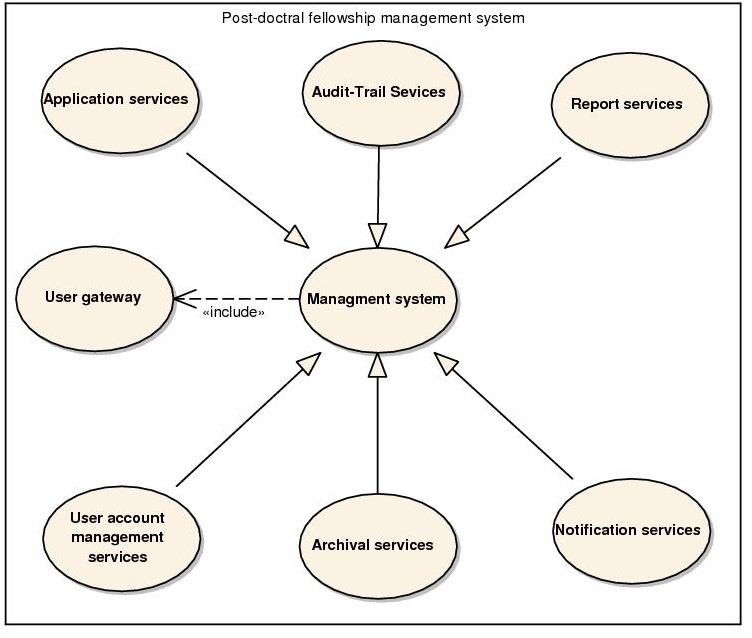
\includegraphics[scale=1]{../Images_Docs/Diagrams/Post-doctral fellowship management system.jpg}}
\caption{Use case diagram of Post-doctoral fellowship management system}
\end{figure}

\begin{figure}[H]
\centering	
\framebox{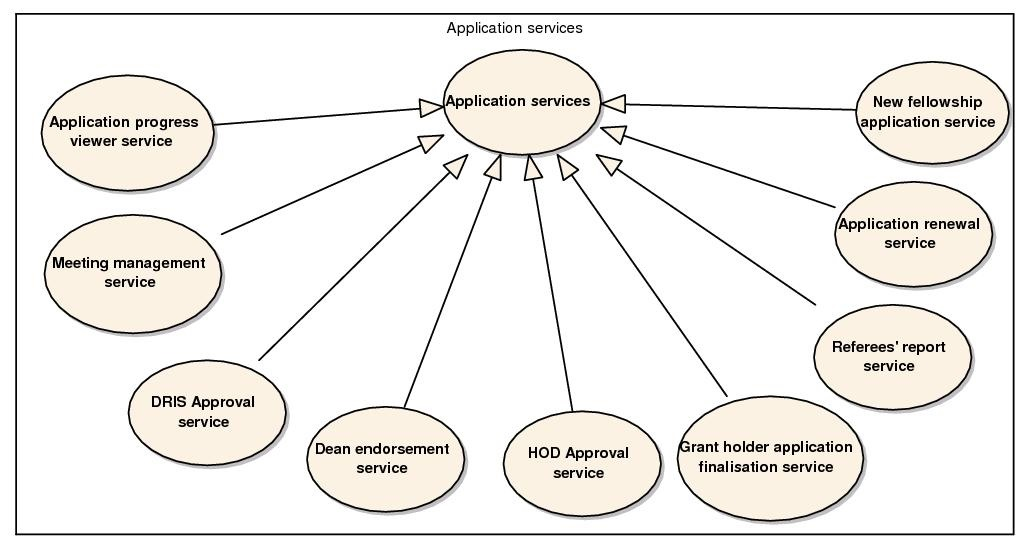
\includegraphics[scale=1]{../Images_Docs/Diagrams/Application services.jpg}}
\caption{Use case diagram of Application service}
\end{figure}

\begin{figure}[H]
\centering	
\framebox{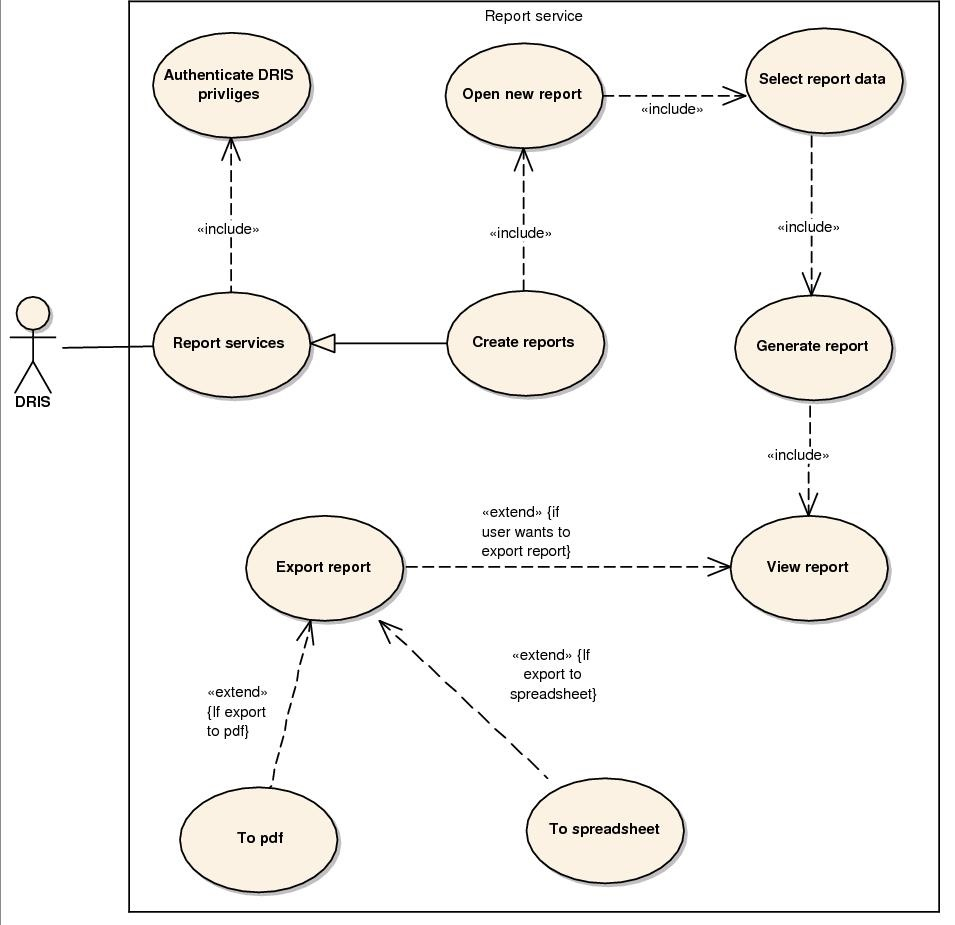
\includegraphics[scale=0.6]{../Images_Docs/Diagrams/Report services.jpg}}
\caption{Use case diagram of Report service}
\end{figure}

\begin{figure}[H]
\centering	
\framebox{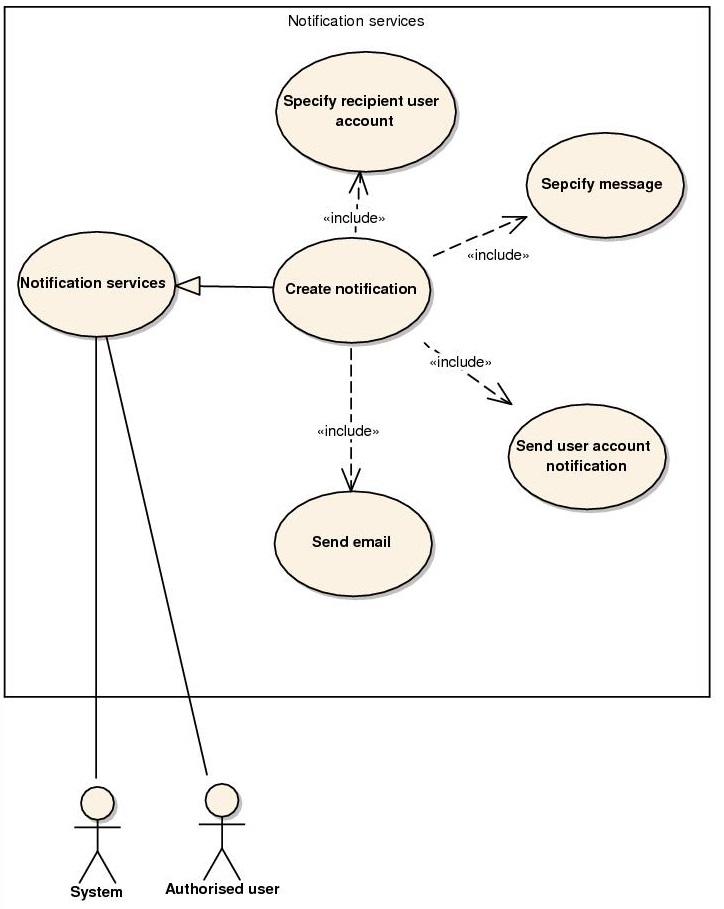
\includegraphics[scale=0.6]{../Images_Docs/Diagrams/Notification services.jpg}}
\caption{Use case diagram of Notification services}
\end{figure}

\begin{figure}[H]
\centering	
\framebox{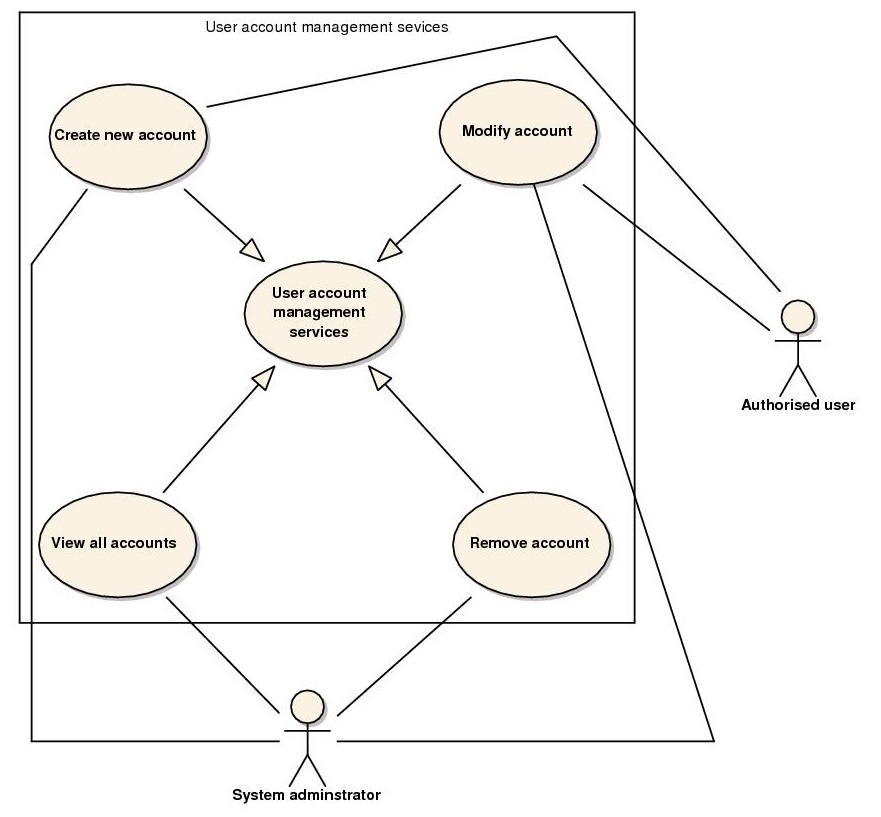
\includegraphics[scale=0.75]{../Images_Docs/Diagrams/User account management services.jpg}}
\caption{Use case diagram of User account management services}
\end{figure}

\begin{figure}[H]
\centering	
\framebox{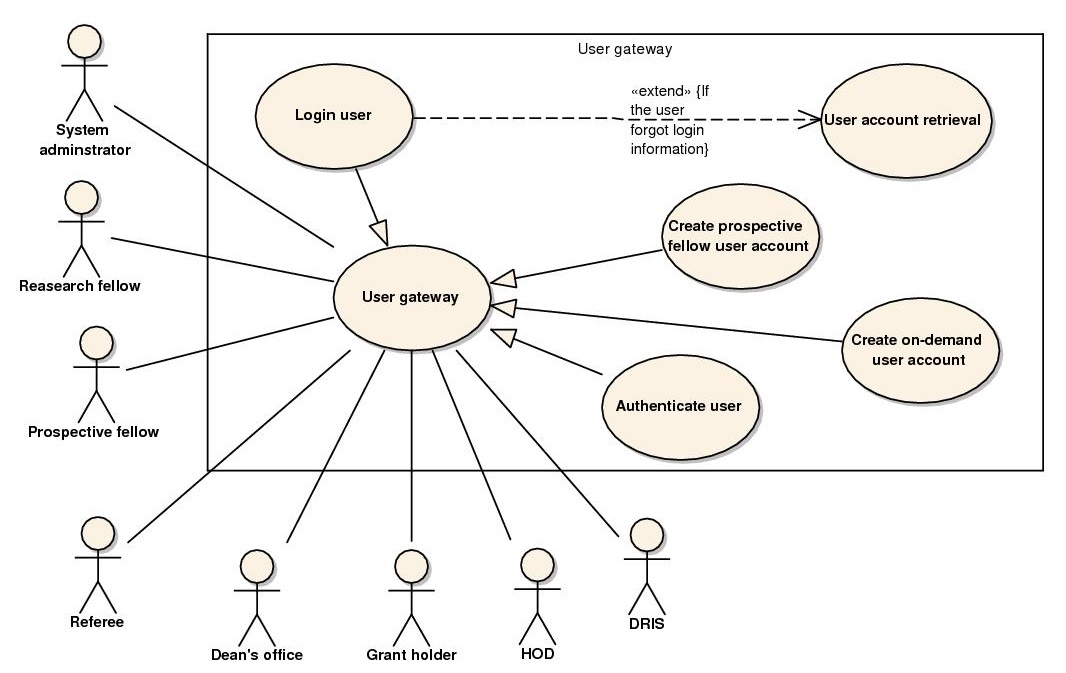
\includegraphics[scale=0.75]{../Images_Docs/Diagrams/User gateway.jpg}}
\caption{Use case diagram of User gateway}
\end{figure}

\begin{figure}[H]
\centering	
\framebox{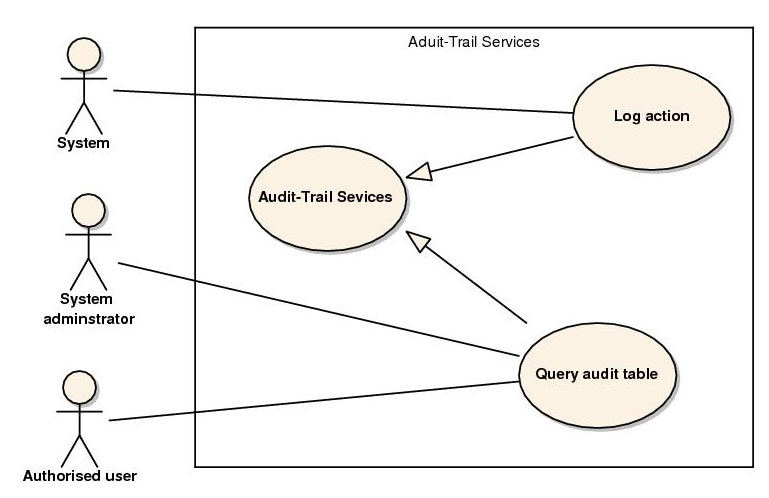
\includegraphics[scale=1]{../Images_Docs/Diagrams/Audit-Trail services.jpg}}
\caption{Use case diagram of Audit-Trail services}
\end{figure}

\begin{figure}[H]
\centering	
\framebox{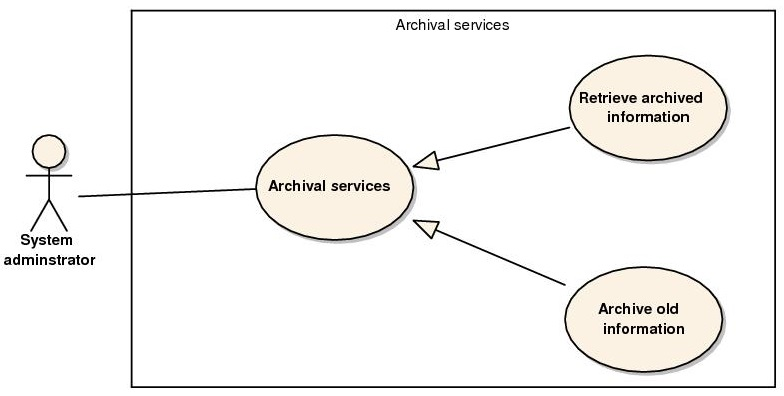
\includegraphics[scale=1]{../Images_Docs/Diagrams/Archival services.jpg}}
\caption{Use case diagram of Archival services}
\end{figure}

\begin{figure}[H]
\centering	
\framebox{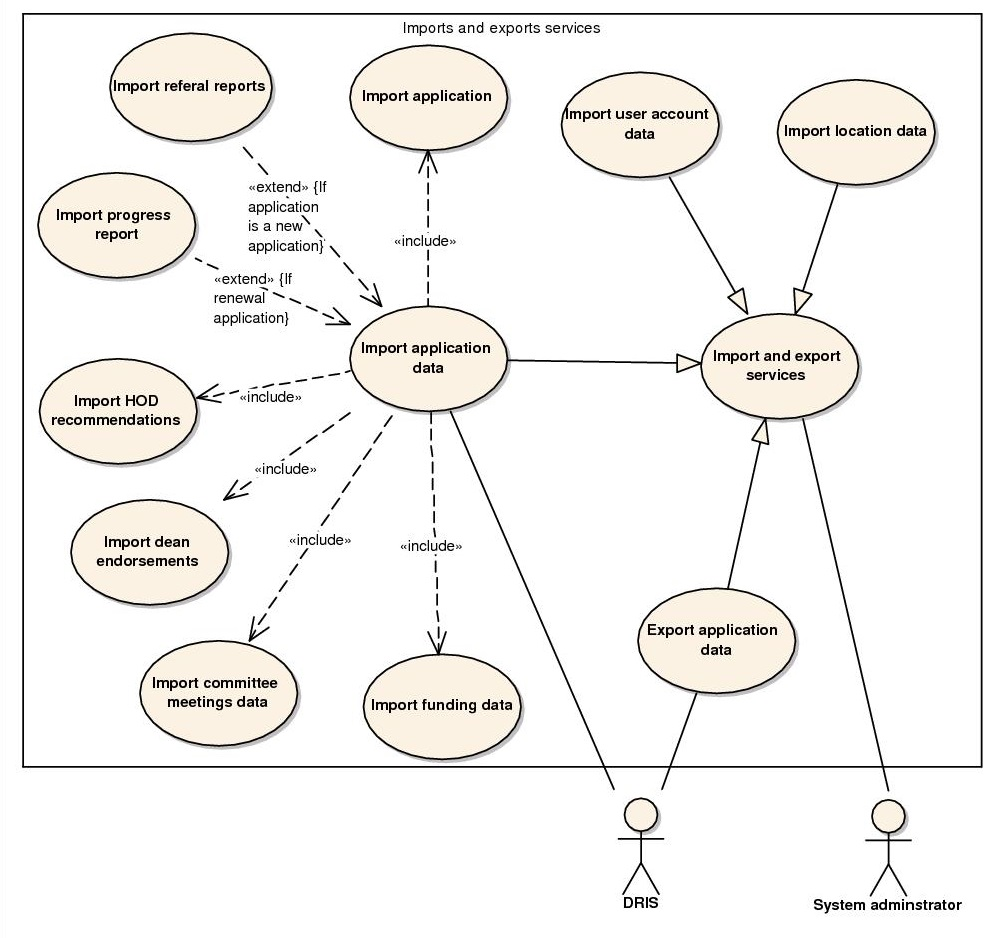
\includegraphics[scale=0.8]{../Images_Docs/Diagrams/Imports and exports services.jpg}}
\caption{Use case diagram of Imports and exports services}
\end{figure}

\begin{figure}[H]
\centering	
\framebox{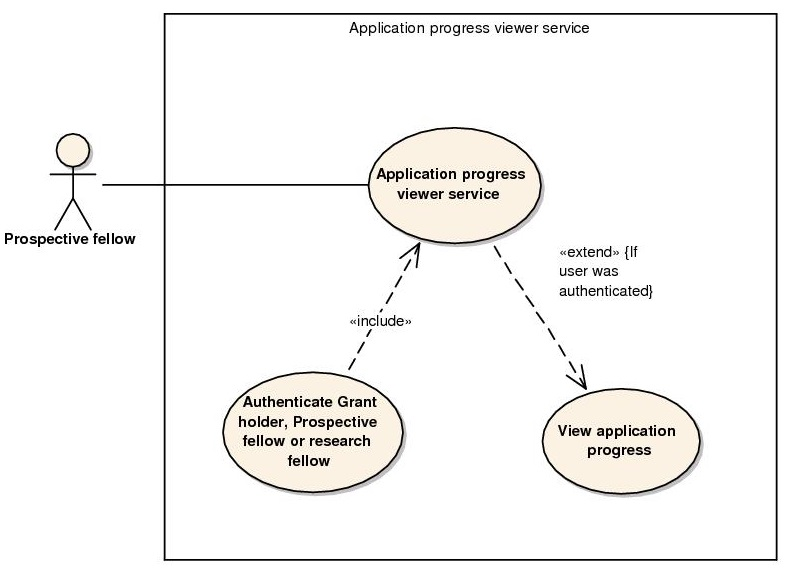
\includegraphics[scale=1]{../Images_Docs/Diagrams/Application/Application progress viewer service.jpg}}
\caption{Use case diagram of Application progress viewer service}
\end{figure}

\begin{figure}[H]
\centering	
\framebox{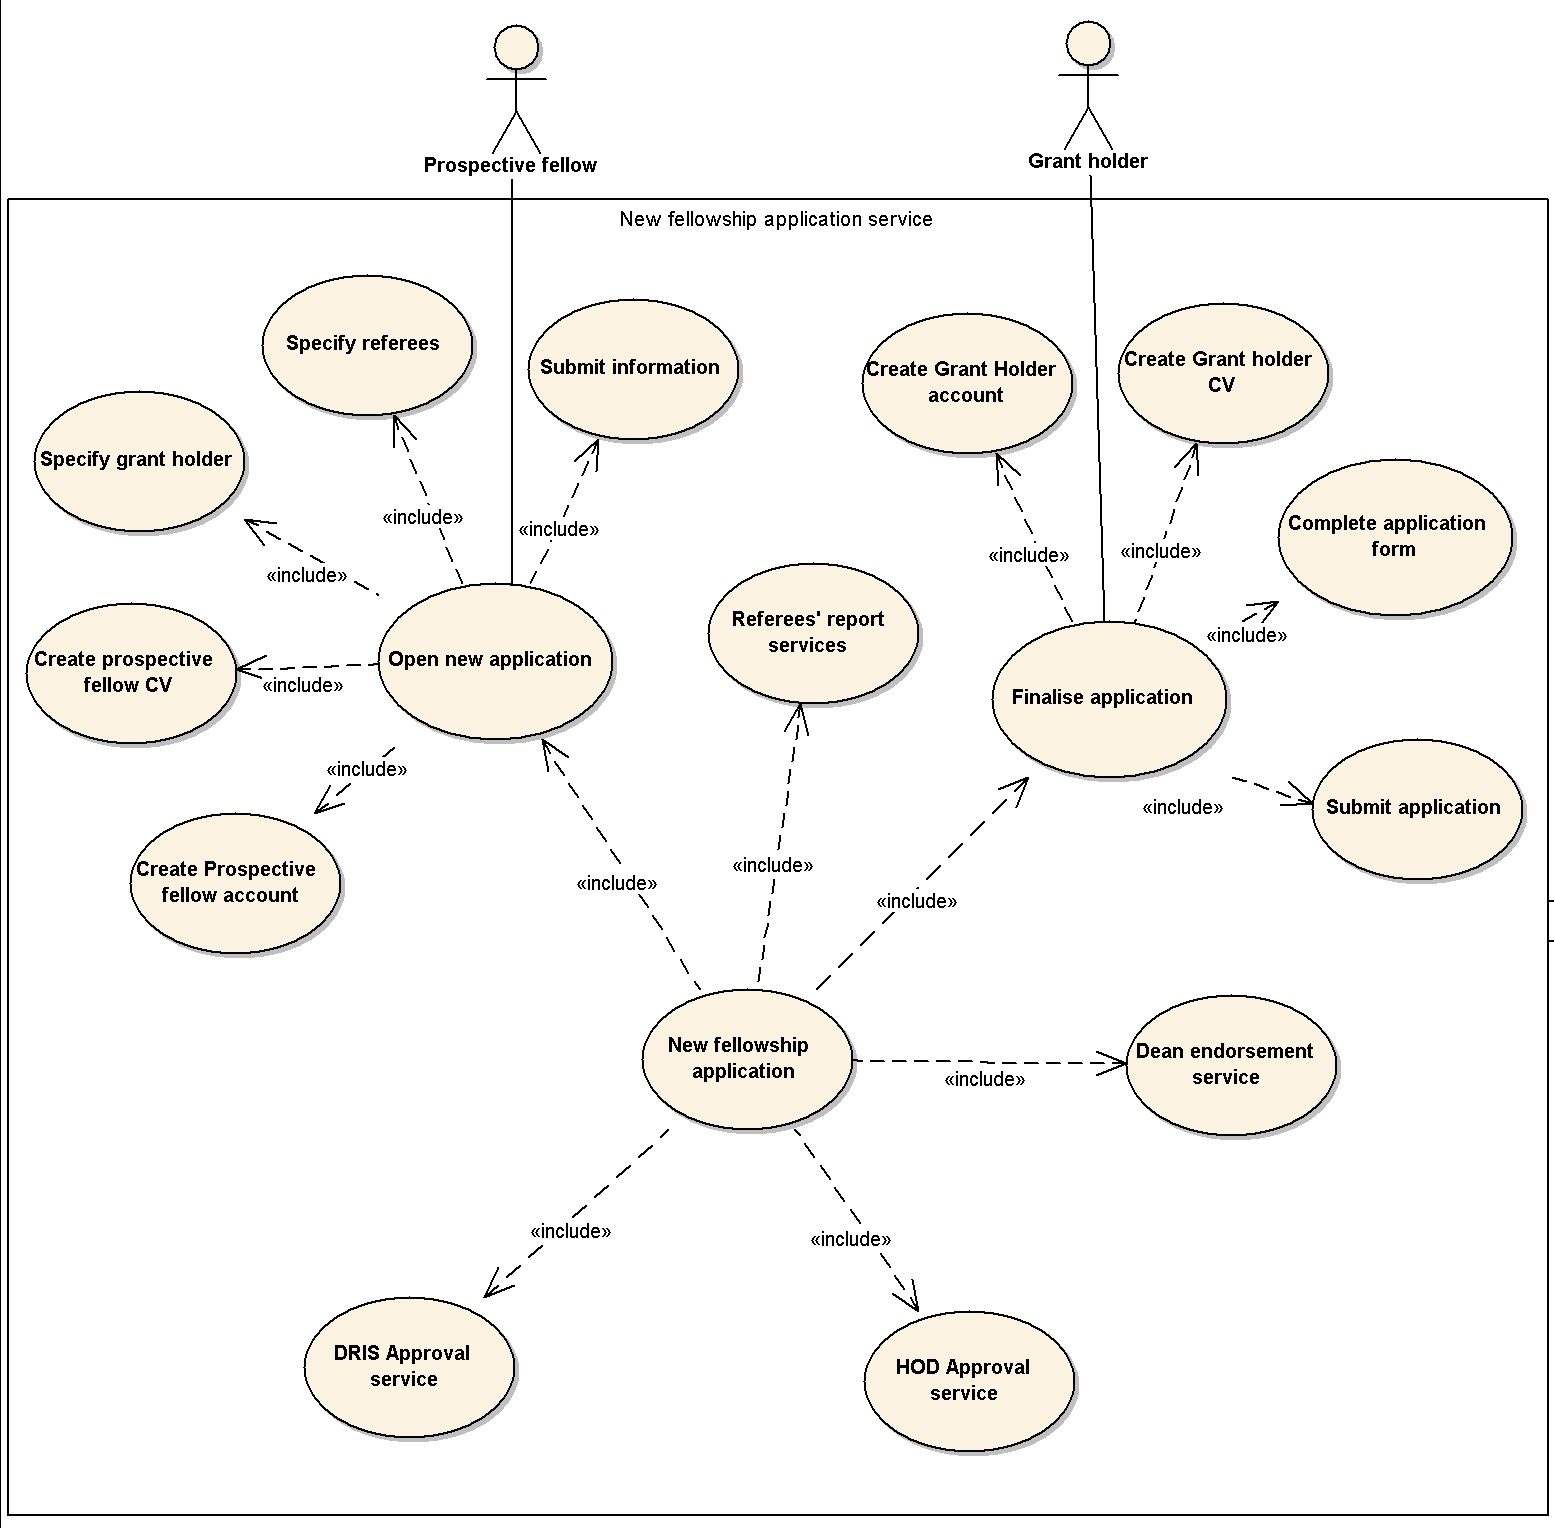
\includegraphics[scale=0.9]{../Images_Docs/Diagrams/Application/New fellowship application service.jpg}}
\caption{Use case diagram of New fellowship application service}
\end{figure}

\begin{figure}[H]
\centering	
\framebox{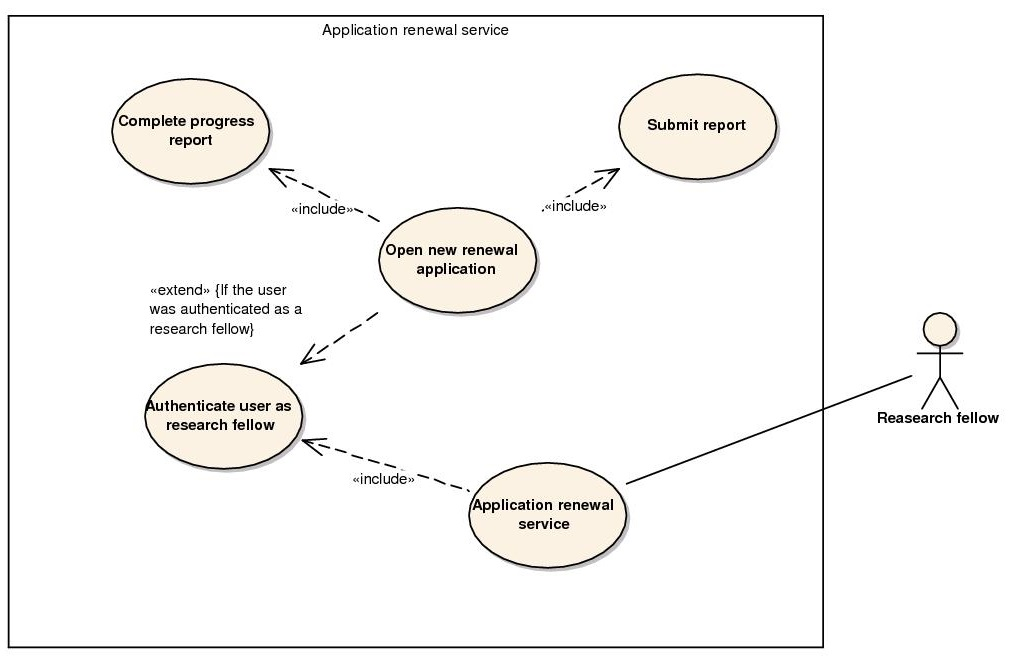
\includegraphics[scale=0.8]{../Images_Docs/Diagrams/Application/Application renewal service.jpg}}
\caption{Use case diagram of Application renewal service}
\end{figure}

\begin{figure}[H]
\centering	
\framebox{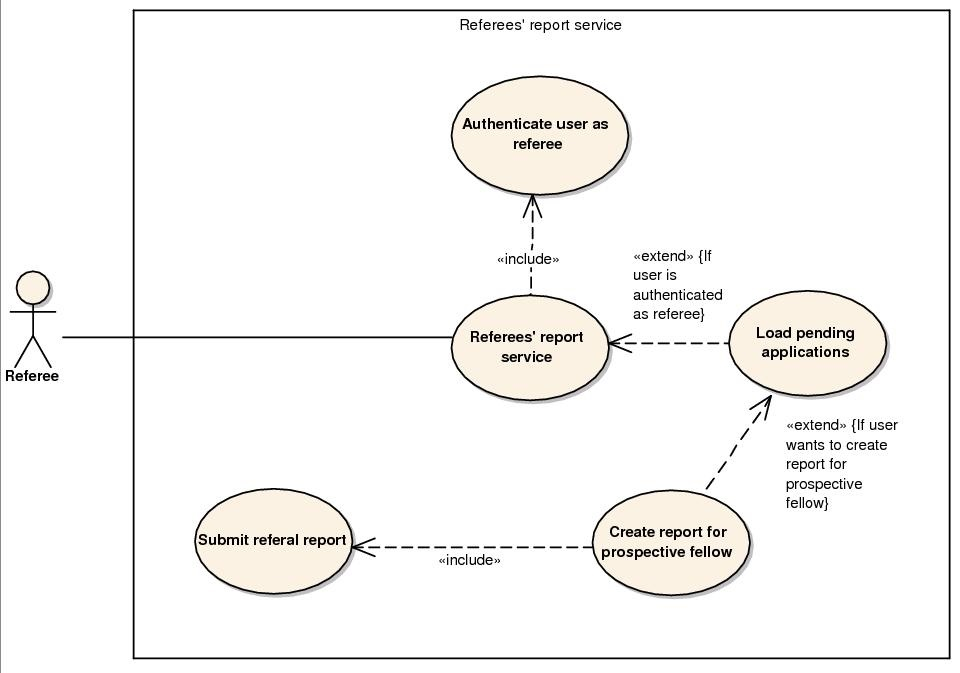
\includegraphics[scale=0.8]{../Images_Docs/Diagrams/Application/Referees' report service.jpg}}
\caption{Use case diagram of Referees' report service}
\end{figure}

\begin{figure}[H]
\centering	
\framebox{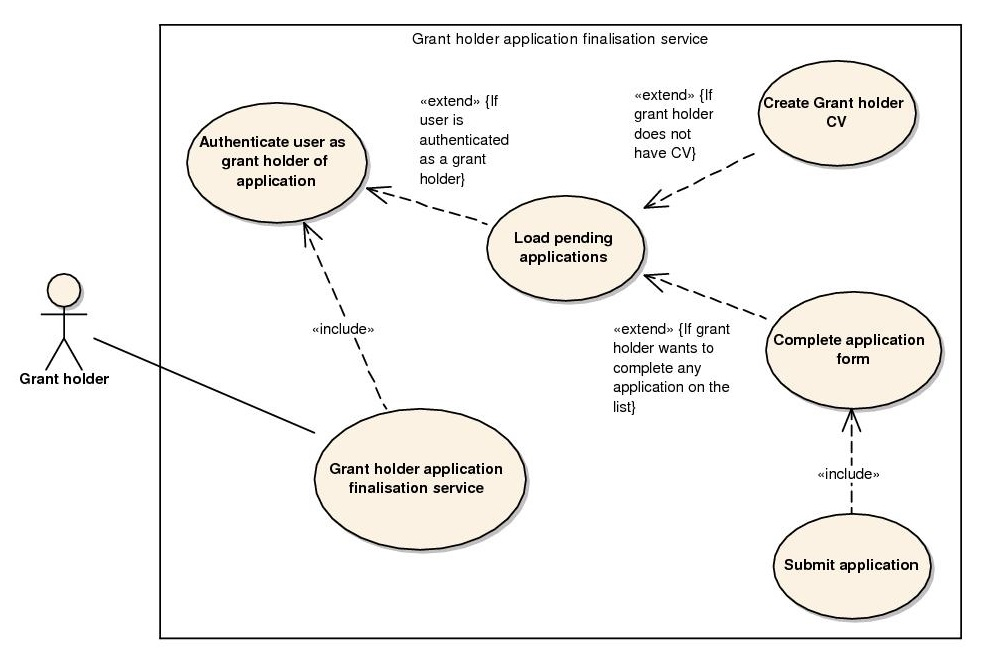
\includegraphics[scale=0.75]{../Images_Docs/Diagrams/Application/Grant holder application finalisation service.jpg}}
\caption{Use case diagram of Grant holder application finalisation service}
\end{figure}

\begin{figure}[H]
\centering	
\framebox{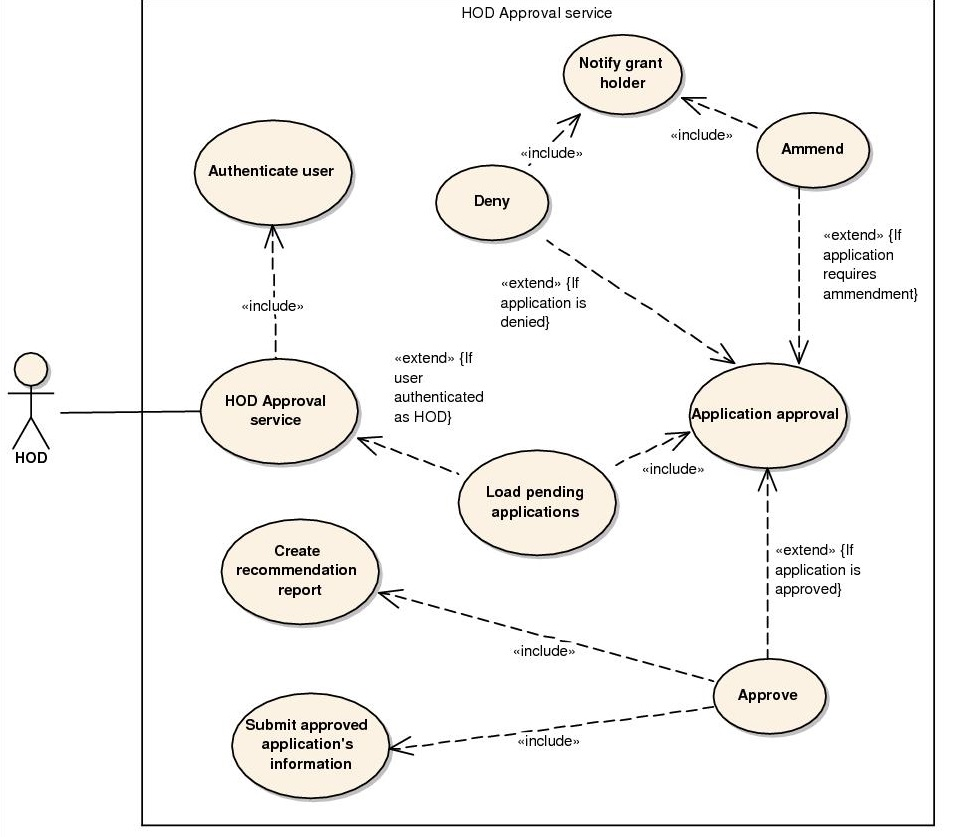
\includegraphics[scale=0.75]{../Images_Docs/Diagrams/Application/HOD Approval service.jpg}}
\caption{Use case diagram of HOD Approval service}
\end{figure}

\begin{figure}[H]
\centering	
\framebox{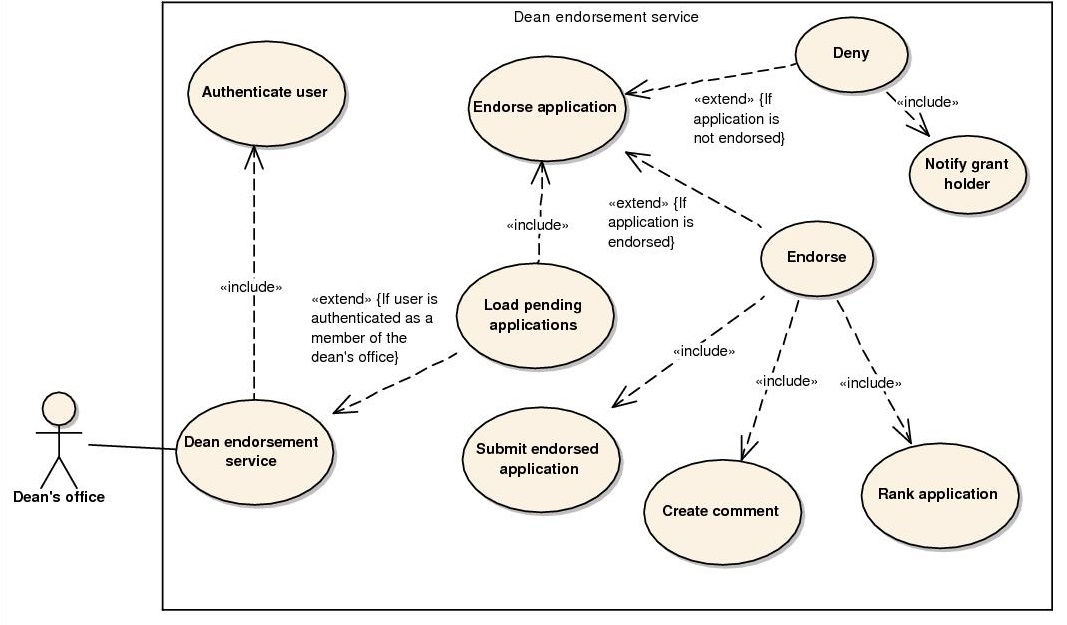
\includegraphics[scale=0.7]{../Images_Docs/Diagrams/Application/Dean endorsement service.jpg}}
\caption{Use case diagram of Dean endorsement service}
\end{figure}

\begin{figure}[H]
\centering	
\framebox{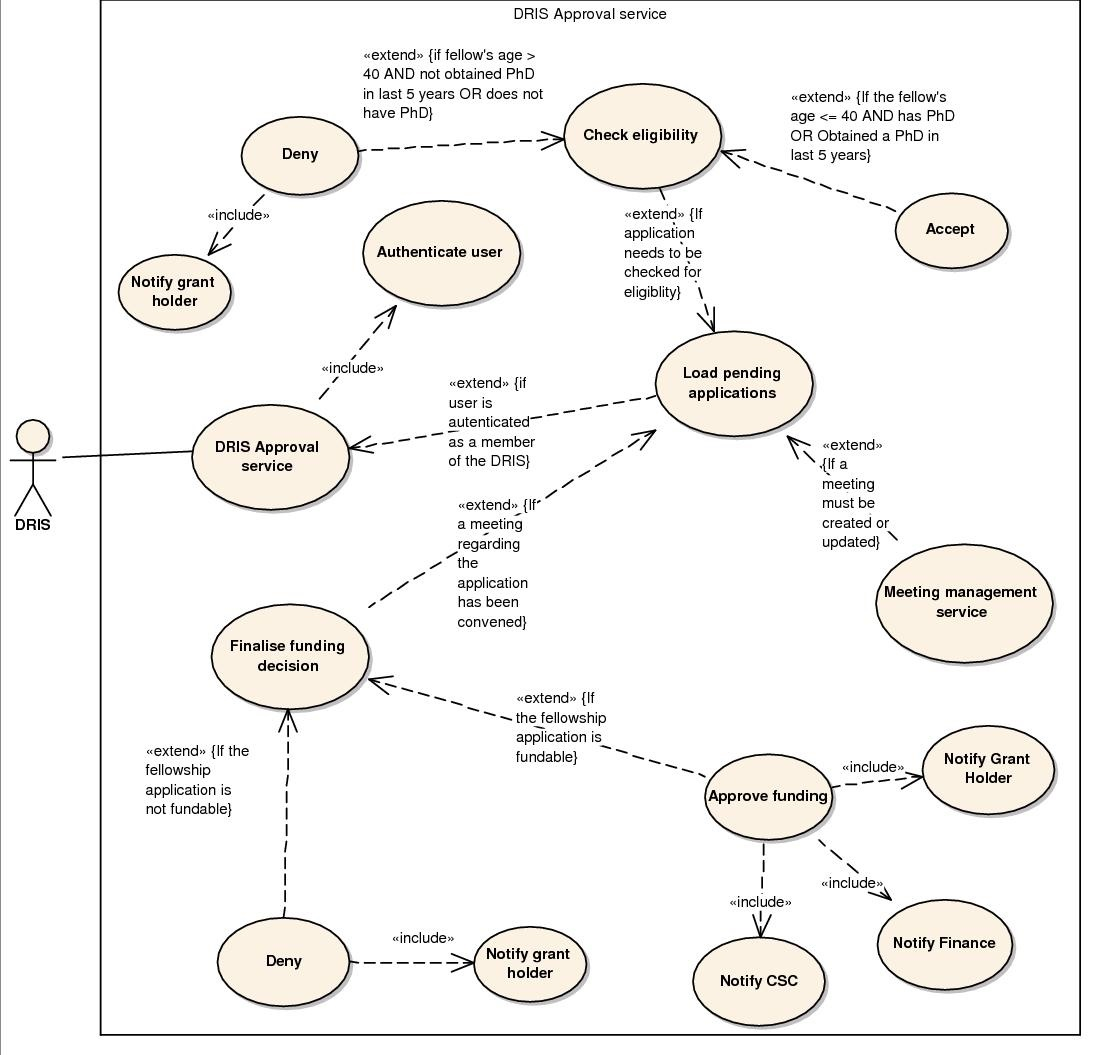
\includegraphics[scale=0.7]{../Images_Docs/Diagrams/Application/DRIS approval service.jpg}}
\caption{Use case diagram of DRIS approval service}
\end{figure}

\begin{figure}[H]
\centering	
\framebox{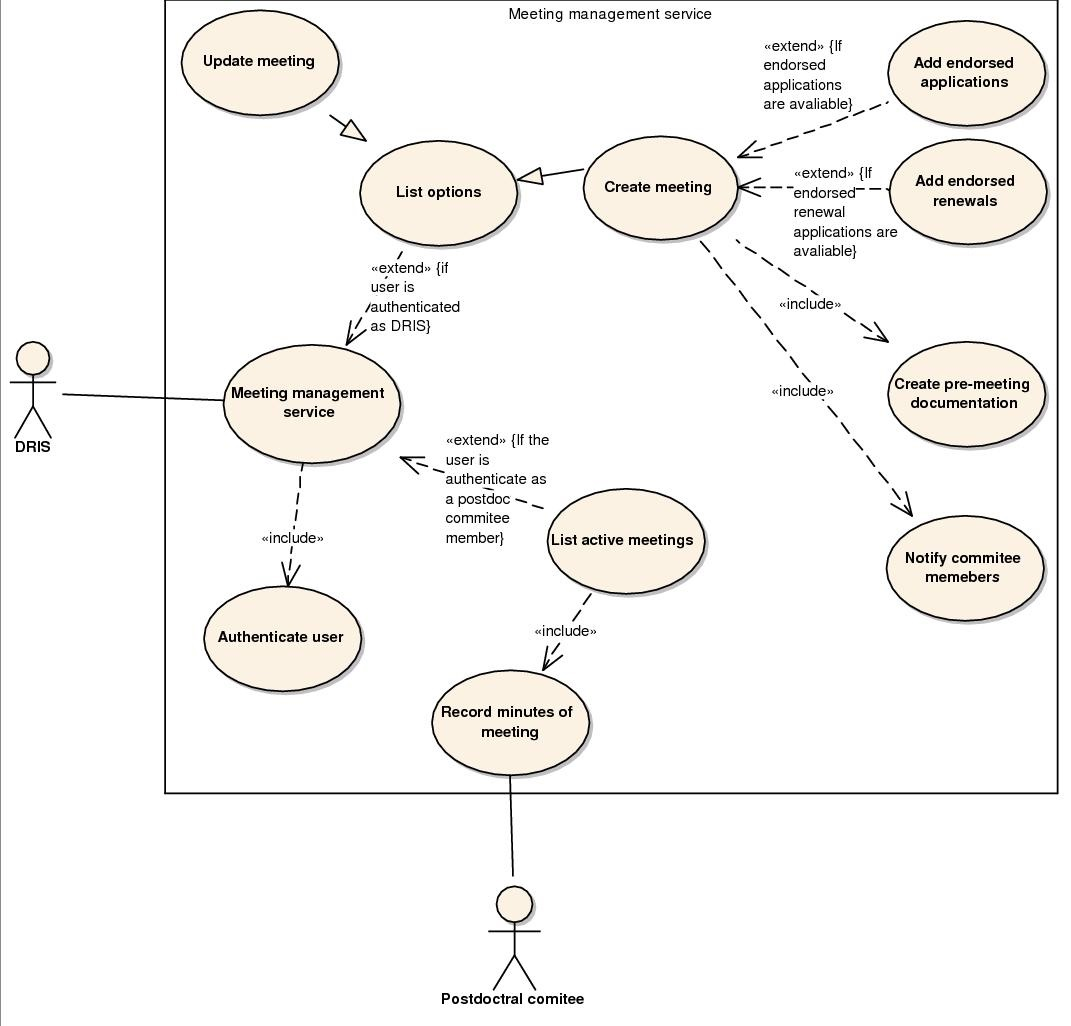
\includegraphics[scale=0.9]{../Images_Docs/Diagrams/Application/Meeting management service.jpg}}
\caption{Use case diagram of Meeting management service}
\end{figure}

\newpage
\subsection{Use case prioritization}
\vspace{0.2in}
This section states the ranking in terms of priority of the service use case per use case diagram figure. The priorities are: Critical, Important and Nice to have.\\ 
\begin{itemize}
	\item User gateway: Critical
	\begin{itemize}
		\item Login user: Critical
		\item User account retrieval: Important
		\item Create prospective fellow user account: Critical
		\item Generate on-demand user account: Critical
		\item Activate on-demand user account: Critical
		\item Authenticate user: Critical
	\end{itemize}
	\item Application services: Critical
	\begin{itemize}
		\item New fellowship application service: Critical
		\item Application renewal service: Critical
		\item Referees' report service: Critical
		\item Grant holder application finalisation service: Critical
		\item HOD Approval service: Critical
		\item Dean endorsement service: Critical
		\item DRIS approval service: Critical		
		\item Meeting management service: Important
		\item Application progress viewer service: Important
	\end{itemize}
	\item Report services: Important
	\item Notification services: Critical
	\item User account management services: Critical
	\begin{itemize}
		\item Create new account: Critical
		\item Modify account: Critical
		\item Remove account: Important
		\item View all accounts: Important
	\end{itemize}
	\item Audit-Trail services: Critical
	\begin{itemize}
		\item Log action: critical
		\item Query audit table: Important
	\end{itemize}
	\item Archival services: Nice to have
	\begin{itemize}
		\item Retrieve archived information: Nice to have
		\item Archive old information: Nice to have
		\item Backup database: Important
	\end{itemize}
	\item Imports and exports services: Important
	\begin{itemize}
		\item Import user account data: Important
		\item Import application data: Nice to have
		\item Import location data: Important
		\item Export application data: Important
	\end{itemize}
	
\end{itemize}


\vspace{0.2in}

\subsection{Use case/Services contracts} %Mathys
\vspace{0.2in}

This section states the preconditions and postconditions of the each use case per use case diagram figure. \\

\subsubsection{Preconditions}
These are conditions that must be met by the system or user before they are allowed to use the use case.\\
\begin{itemize}
	\item Fig 2.
		\begin{itemize}
			\item New fellowship application service: Can only be accessed if new applications are open.
			\item Application renewal service: Can only be accessed if renewals are open and if the user is a research fellow that is still in possession of a fellowship.
			\item Referees' report service:  Can only be accessed if user is a referee.
			\item Grant holder application finalisation service:  Can only be accessed if user is a grant holder.
			\item HOD Approval service:  Can only be accessed if user is a HOD.
			\item Dean endorsement service:  Can only be accessed if user is a member of the dean's office.
			\item DRIS Approval service:  Can only be accessed if user is a member of the DRIS.
			\item Meeting management service:  Can only be accessed if user is a member of the DRIS or post-doctoral committee member.
			\item Application progress viewer service: Can only be accessed if user logged as a prospective fellow, research fellow or grant holder. Also the user needs to have at least one application on the system.	
		\end{itemize}
	
	\item Fig 3.
		\begin{itemize}
			\item Create report: If a user with the associated credentials has been authenticated as a member of the DRIS or with the correct security role.
			\item Open new report: If no report is currently open.
			\item Select report data: If report is open and data is available for report.
			\item Generate report: If data has been selected.
			\item View report: If a report has been generated.
			\item Export report: If user wants to export report and the user is busy viewing the report.
			\item To spreadsheet: If user wants to export report to a spreadsheet.
			\item To pdf: If user wants to export report to a pdf.	
		\end{itemize}
	
	\item Fig 4.
		\begin{itemize}
			\item Create notification: If requesting user is the system or an authorised user.
			\item Specify recipient user account: If a notification is in its setup stage.				
			\item Specify message: If a notification is in its setup stage.
			\item Send user account notification: If notification is ready to be sent.
			\item Send email: If notification is ready to be sent.	
		\end{itemize}
	
	\item Fig 5.
		\begin{itemize}
			\item Create new account: If requesting user has the appropriate security role.
			\item Modify account: If requesting user has the appropriate security role or is the owner of the account.				
			\item Remove account: If requesting user has the appropriate security role.	
			\item View all accounts: If requesting user is a system administrator.					
		\end{itemize}
	
	\item Fig 6.
		\begin{itemize}
			\item Login user: If requesting user is a user of the system.
			\item User account retrieval: If requesting user has forgotten their user credentials.				
			\item Create prospective fellow account: If a new prospective fellow wishes to create an account.	
			\item Activate on-demand user account: If a user has been identified by an applicant and has a security token.
			\item Authenticate user: if user is logged in.						
		\end{itemize}
	
	\item Fig 7.
		\begin{itemize}
			\item Log action: If requesting user is the system.
			\item Query audit table: If the user has the correct security role.										
		\end{itemize}
	\item Fig 8.
		\begin{itemize}
			\item Retrieve archived information: If requesting user is a system administrator or the system.
			\item Archive old information: If requesting user is a system administrator or the system.	
			\item Backup database: If requesting user is a system administrator.					
		\end{itemize}
	\item Fig 9.
		\begin{itemize}
			\item Import application data: If requesting user is a system administrator or a DRIS member.
			\item Export application data: If requesting user is a system administrator or a DRIS member.	
			\item Import location data: If requesting user is a system administrator.
			\item Import faculty information: If no such faculty is in the database already.
			\item Import departments information: If no such department is in the database and the faculty it relates to is in the database.
			\item Import user account data: If requesting user is a system administrator.
			\item Populate user account data: If the user account exists in th e database and the data is valid.
			\item Import referral reports: If the application is a new application.
			\item Import progress report: If the application is a renewal application.
			\item Import HOD recommendations: If the application has a valid HOD recommendation.
			\item Import dean endorsements: If the application has a valid dean's endorsement.
			\item Import DRIS approval data: If the application has valid DRIS approval data.
			\item Import funding data: If the application has a valid funding data and has been funded.				
		\end{itemize}		
	\item Fig 10.
		\begin{itemize}
			\item View application progress: Can only be used if there are any applications made by the user.
		\end{itemize}
		
	\item Fig 11.
		\begin{itemize}
			\item Generate on-demand user account: If the prospective fellow has identified a referee or grant holder not on the system.
			\item Submit information: If all the application information is complete.
		\end{itemize}
	
	\item Fig 12.
		\begin{itemize}
			\item Open new renewal application: If research fellow has a fellowship that is renewable.
			\item Submit report: If the progress report has been completed.				
			\item Submit renewal application: If all the required information for the renewal has been entered.									
		\end{itemize}
	
	\item Fig 13.
		\begin{itemize}
			\item Load pending applications: If there are any pending applications for the referee and if the user was authenticated as the referee.
			\item Create report: If if a application is selected from the list of pending applications.				
			\item Submit referral report: If the referral report has been completed.									
		\end{itemize}
		
	\item Fig 14.
		\begin{itemize}
			\item Load pending applications: If there are any pending applications for the grant holder and if the user was authenticated as the grant holder.
			\item Create Grant holder CV: If grant holder does not have a CV.
			\item Complete application form: If grant holder has selected any application that is still pending.
			\item Submit application: If all the required information has been entered									
		\end{itemize}
		.	
	\item Fig 15.
		\begin{itemize}
			\item Load pending applications: If there are any finalised application available for approval and the grant holder of the application falls under department the HOD is in charge of and if user has been authenticated as the HOD.
			\item Application approval: If HOD has selected a application from the application list. 
			\item Create recommendation report: If the application has been approved.				
			\item Submit approved application's information: If the recommendation report has been completed.									
		\end{itemize}
		
	\item Fig 16.
		\begin{itemize}
			\item Load pending applications: If there are any approved application available for endorsement and the grant holder of the application falls under faculty of which the Dean's office is in charge of and the user has been authenticated as a member of the dean's office.
			\item Endorse application: If a application is selected from the pending list. 
			\item Rank application: If the application has been endorsed.	
			\item Create comment: If the application has been ranked.			
			\item Submit endorsed application: If the required endorsement information has been completed.									
		\end{itemize}
	
	\item Fig 17.
		\begin{itemize}
			\item Load pending applications: If the user is authenticated as a member of the DRIS and if there are any endorsed application available for eligibility checking or applications available for finalising their funding decisions.
			\item Check eligibility: If there are any endorsed application available for its eligibility check.
			\item Deny: If the prospective fellow is older than 40 and has not obtained their PhD in the last 5 years or if the prospective fellow does not have a PhD.
			\item Accept: If the prospective fellow is younger than 40 or is 40 and they have a PhD or if they have obtained a PhD in the last 5 years.
			\item Meeting management service: If a meeting is to be created or updated. 
			\item Finalise funding decision: If the meeting regarding the application has been concluded.
			\item Create funding information: The application has been approved for funding.	
			\item Deny: If the application's funding was denied.			
			\item Approve funding: If the application's funding was denied.									
		\end{itemize}
	
	\item Fig 18.
		\begin{itemize}
			\item List options: If user is a authenticated DRIS member.
			\item Create meeting: If any eligible applications are available and the user selects the service from the options list.
			\item Add endorsed applications: If any new applications that are eligible are available.
			\item Add endorsed renewals: If any renewal applications that are eligible are available.
			\item List active meetings: If user is a authenticated post doctoral committee member.
			\item Record minutes of meeting: If the selected meeting has been listed.							
		\end{itemize}
	\end{itemize}

\subsubsection{Postconditions}
These are conditions that must be met by the system and the data after the use case has been used.\\
\begin{itemize}
		
	\item Fig 3.
		\begin{itemize}
			\item Authenticate user: The user has been authenticated as a DRIS member or has the appropriate security role.
			\item Open new report: A new report is active.
			\item Select report data: The data for the active report is selected.
			\item Generate report: The report is available for viewing.
			\item View report: The report is available for export and must be visible.	
		\end{itemize}
	
	\item Fig 4.
		\begin{itemize}
			\item Authenticate user: The user was authenticated as the system or a user with the appropriate security role.
			\item Create notification: A possible notification is open for receiving its contents.
			\item Specify recipient user account: The notification has a a recipient.				
			\item Specify message: The notification has a message.
			\item Send user account notification: The message is sent to the user.
			\item Send email: The message is sent the email associated with recipients user account.	
		\end{itemize}
	
	\item Fig 5.
		\begin{itemize}
			\item Create new account: A new user account is added to the system.
			\item Modify account: The specified user account is updated.				
			\item Remove account: The specified user account is removed from the system.
			\item View all accounts: All user accounts are listed.						
		\end{itemize}
	
	\item Fig 6.
		\begin{itemize}
			\item Login user: User is verified and logged in.
			\item User account retrieval: An recovery email is sent to the user account that has been queried for recovery.				
			\item Create prospective fellow user account: A prospective fellows user account was created.
			\item Generate on-demand user account: A user account identified by the system and account security token was created.
			\item Activate on-demand user account: The on-demand account has been confirmed is active.
			\item Authenticate user: The user is confirmed to be logged in and has the security role expected by the system.						
		\end{itemize}
		
	\item Fig 7.
		\begin{itemize}
			\item Log action: A user action was recorded in the audit table and cannot be changed by user nor by the system.
			\item Query audit table: An valid response to the query was returned.									
		\end{itemize}
	\item Fig 8.
		\begin{itemize}
			\item Retrieve archived information: The current working database has been repopulated with the selected archive database data.
			\item Archive old information: Any old information in the current working database is moved to the archived database.
			\item Backup database: The database has been backed up the specified location.									
		\end{itemize}
	\item Fig 9.
		\begin{itemize}
			\item Import application data: All the specified application data is now in the database.
			\item Export application data: All the specified application data has been exported.	
			\item Import location data: All the specified location data is now available in the database. 
			\item Import faculty information: The specified faculty is now in the database.
			\item Import departments information: The specified department is now in the database.
			\item Import user account data: The user account has been created on the system and the user is notified of this.
			\item Populate user account data: The data of the user has been imported into the new user account.
			\item Import referral reports: The associated application's referral reports are in the database.
			\item Import progress report: The associated application's progress report is in the database.
			\item Import HOD recommendations: The associated application's HOD recommendation is in the database.
			\item Import dean endorsements: The associated application's dean endorsement is in the database.
			\item Import DRIS approval data: The associated application's DRIS approval data is in the database.
			\item Import funding data: The associated application's funding data is in the database.				
		\end{itemize}
	\item Fig 10.
		\begin{itemize}
			\item Authenticate user: The current user was authenticated as a grant holder or research fellow or a prospective fellow.
			\item View application progress: The application progress of the specified user application is visible.									
		\end{itemize}				
		
	\item Fig 11.
		\begin{itemize}
			\item Authenticate user: The current user was authenticated as a prospective fellow.
			\item Create prospective fellow cv: The CV is created and associated with the prospective fellow.
			\item Specify grant holder: The grant holder's contact information is associated with the application.
			\item Specify referees: The referees' contact information is associated with the application.
			\item Submit information: The initial application data is complete. Referees are notified. And the prospective fellow is a associated with the application.				
		\end{itemize}
	
	\item Fig 12.
		\begin{itemize}
			\item Authenticate user: The current user was authenticated as a research fellow.
			\item Open new renewal application: A new renewal is for a fellowship is open.
			\item Complete progress report: The progress report associated with	the renewal is completed.		
			\item Submit report: The initial renewal information is complete. Grant holder is notified.											
		\end{itemize}
	
	\item Fig 13.
		\begin{itemize}
			\item Authenticate user: The current user was authenticated as a referee.
			\item Load pending applications: Any applications that need a referral report from the specified referee must be listed.
			\item Create report for prospective fellow: The report is complete and ready to be submitted.				
			\item Submit referral report: The referral report has been finalised and associated with the application and the Grant Holder of the application is notified.									
		\end{itemize}
	\item Fig 14.
		\begin{itemize}
			\item Authenticate user: The current user was authenticated as a grant holder.
			\item Load pending applications: Any applications that need to be finalised from the specified grant holder must be listed.
			\item Create report for prospective fellow: The report is complete and ready to be submitted.				
			\item Submit referral report: The referral report has been finalised and associated with the application and the Grant Holder of the application is notified.
			\item Create grant holder cv: The grant holder's CV is associated with the grant holder.
			\item Complete application form: The application data is complete and the application is ready to be finalised.
			\item Submit application: The application is now a finalised application and the grant holder is associated with the application. The HOD of the relative department is notified. 									
		\end{itemize}	
	\item Fig 15.
		\begin{itemize}
			\item Authenticate user: The current user was authenticated as a HOD.
			\item Load pending applications: Any applications that need to be approved by the specified HOD must be listed.
			\item Deny: Application has status changed to denied.
			\item Amend: Application is reopened and status changed to amend.
			\item Notify grant holder: A denied or amend notification is sent to the Grant holder of the application appropriately.  
			\item Approve: The application recommendation report becomes available for completion.
			\item Create recommendation report: The recommendation report is associated with the application and the Approval is ready to be finalised.				
			\item Submit approved application's information: The application approval is finalised and the application is now a approved application and the Dean's Office of the relevant faculty is notified.									
		\end{itemize}
		
	\item Fig 16.
		\begin{itemize}
			\item Authenticate user: The current user was authenticated as a member of a dean's office.
			\item Load pending applications: Any applications that need to be approved by the specified dean's office must be listed.
			\item Deny: The application's status is changed to denied. 
			\item Notify grant holder: A denied notification is sent to the Grant holder of the application.
			\item Endorse: The application's endorsement information becomes available for completion.
			\item Rank application: The application has a rank associated with it.	
			\item Create comment: The application has a endorsement comment associated with it.			
			\item Submit endorsed application: The application endorsement is finalised and the application is now an endorsed application and the DRIS is notified.									
		\end{itemize}
	
	\item Fig 17.
		\begin{itemize}
			\item Authenticate user: The current user was authenticated as a member of the DRIS.
			\item Load pending applications: Any applications that need to be checked for eligibility or have their final funding decision made by the DRIS must be listed.
			\item Deny: The application's status is changed to denied if it is not eligible. 
			\item Notify grant holder: A denied notification is sent to the Grant holder of the application.
			\item Accept: The application is ready for discussion and is now an eligible application.			
			\item Deny: The application's status is changed to denied if its funding is not approved.			
			\item Approve funding: The application is now a complete application.
			\item Create funding information: The application has its funding information associated with it.
			\item Notify grant holder: A notification is sent to the Grant holder of the application that it is successful.
			\item Notify CSC: A customizable notification is sent to the CSC.
			\item Notify Finance: A customizable notification is sent to the Finance department.									
		\end{itemize}
	
	\item Fig 18.
		\begin{itemize}
			\item Authenticate user: The current user was authenticated as a member of the DRIS or the Post doctoral committee.
			\item List options: The option to update or create meeting are listed.
			\item Create meeting: A new meeting is open for modification.
			\item Add endorsed applications: An endorsed new application has been added to the agenda of the meeting.
			\item Add endorsed renewals: An renewal application has been added to the agenda of the meeting.
			\item Create pre-meeting documentation: Documentation complete and associated with meeting and the meeting is closed for modification.
			\item Notify committee members: A notification is sent to all the committee members.
			\item List active meetings: All active meetings at the time are listed.
			\item Record minutes of meeting: The meeting is finalised and it's minutes stored.							
		\end{itemize}

\end{itemize}

\subsubsection{Request and result data structures}
The system will be following a object oriented approach due it being the paradigm of the Java programming language. Therefore the input and output structure will mainly be in the form of objects. Also the objects that will be produced and used inside the system will adhere to the domain objects specification found below.

\vspace{0.2in}
\newpage
\subsection{Process specifications}
\vspace{0.2in}

\begin{figure}[H]
\centering	
\framebox{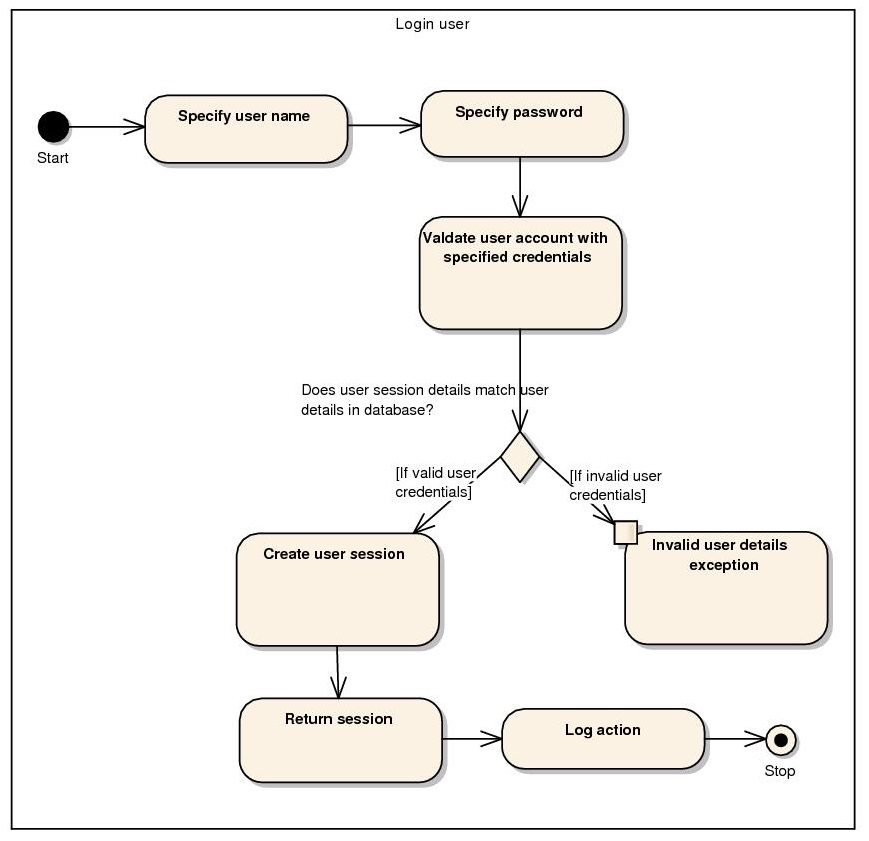
\includegraphics[scale=0.7]{../Images_Docs/Diagrams/Process specs/Login user.jpg}}
\caption{Activity diagram of the Login user use case.}
\end{figure}

\begin{figure}[H]
\centering	
\framebox{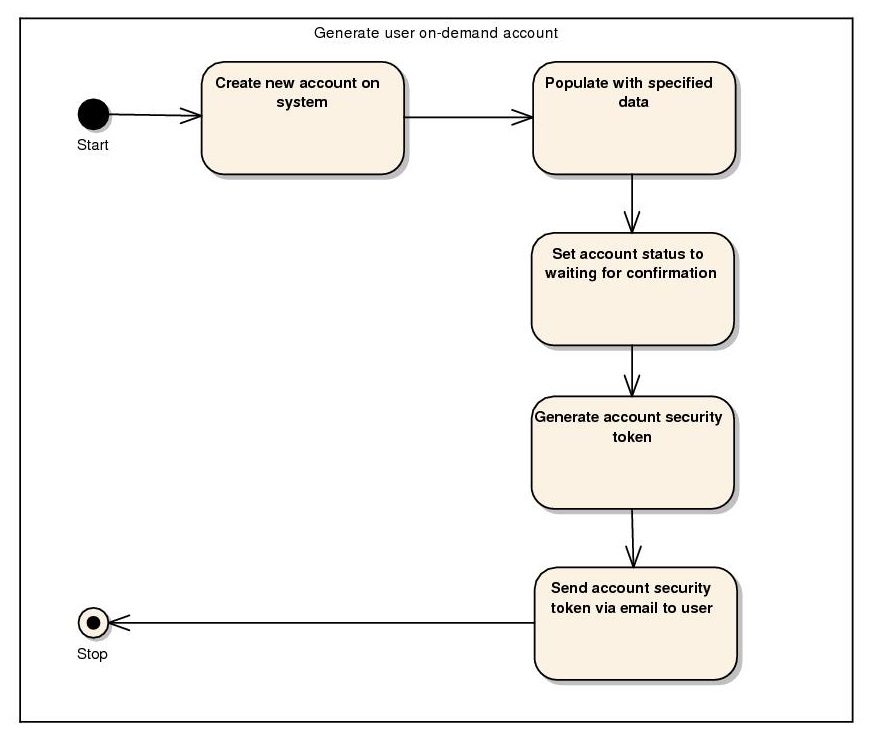
\includegraphics[scale=0.65]{../Images_Docs/Diagrams/Process specs/Generate user on-demand account.jpg}}
\caption{Activity diagram of the Generate user on-demand account use case.}
\end{figure}


\begin{figure}[H]
\centering	
\framebox{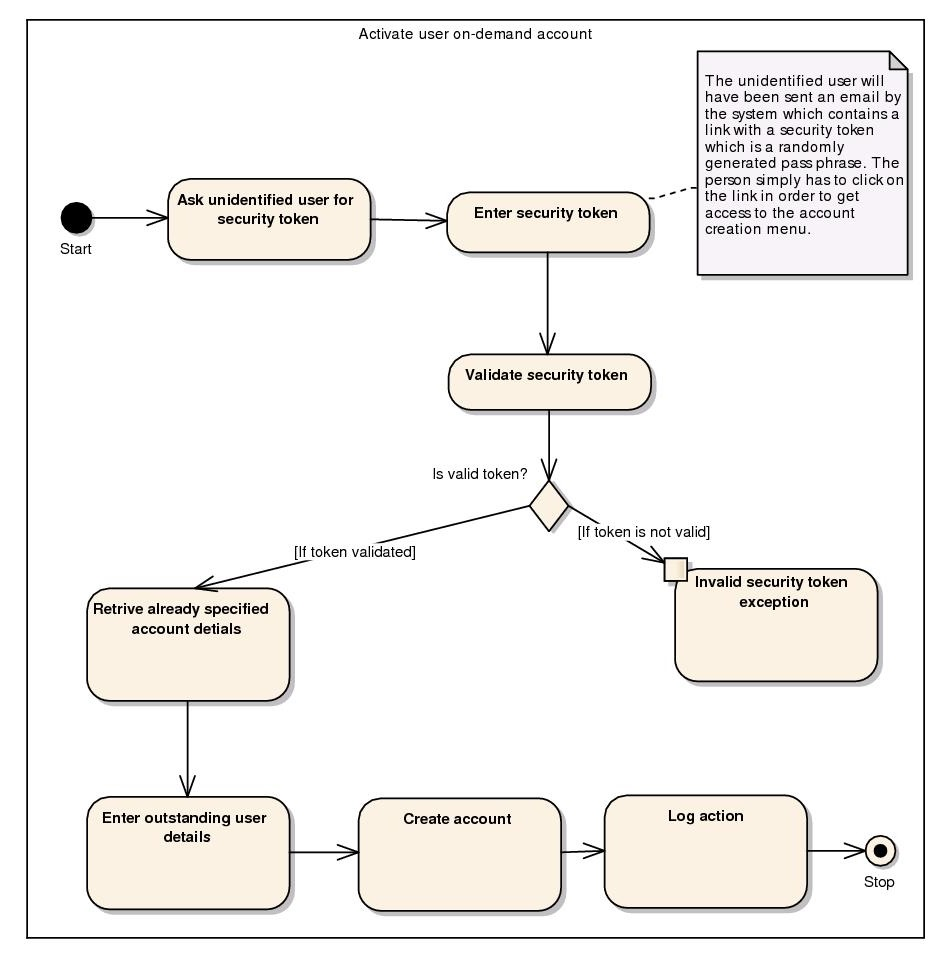
\includegraphics[scale=1]{../Images_Docs/Diagrams/Process specs/Activate user on-demand account.jpg}}
\caption{Activity diagram of the Activate user on-demand account use case.}
\end{figure}

\begin{figure}[H]
\centering	
\framebox{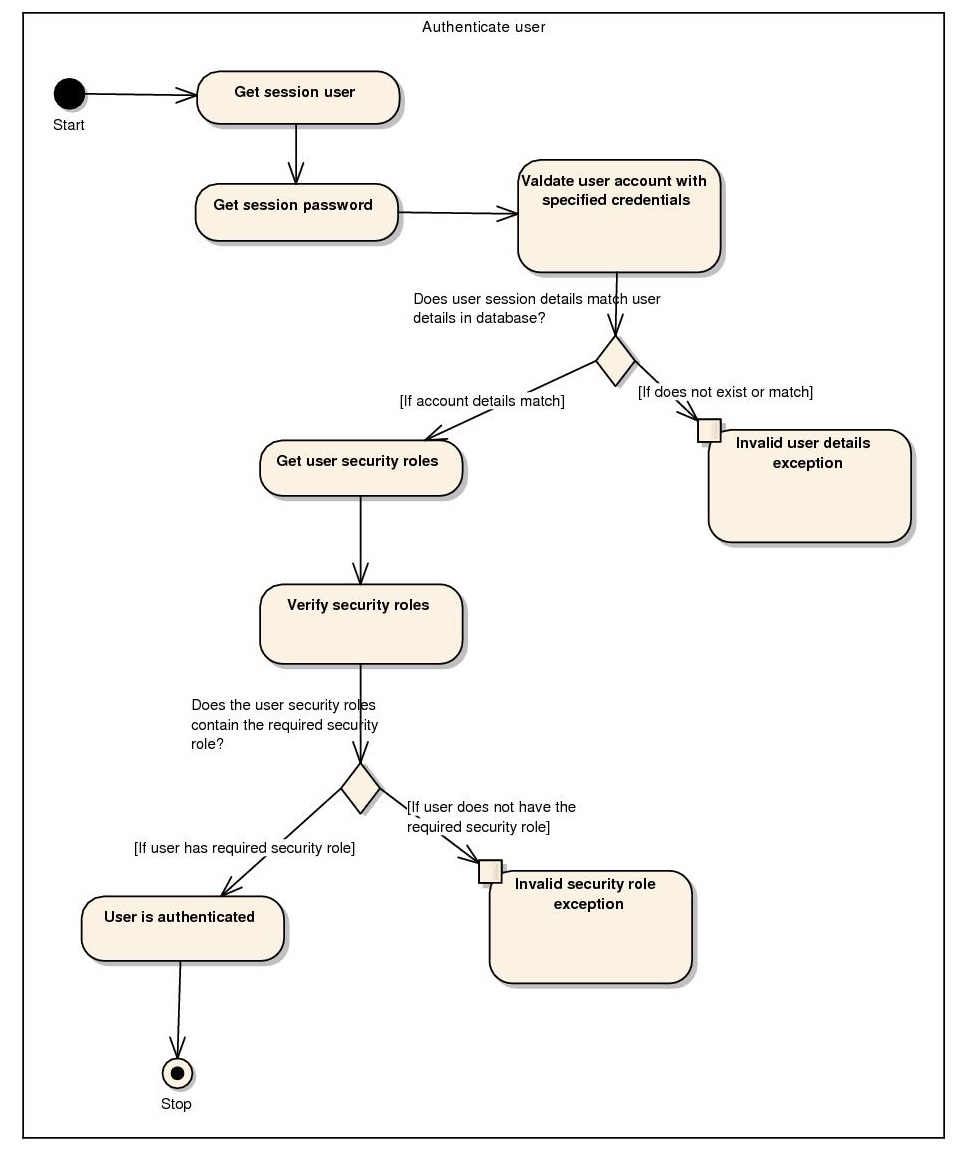
\includegraphics[scale=1]{../Images_Docs/Diagrams/Process specs/Authenticate user.jpg}}
\caption{Activity diagram of the Authenticate user use case.}
\end{figure}

\begin{figure}[H]
\centering	
\framebox{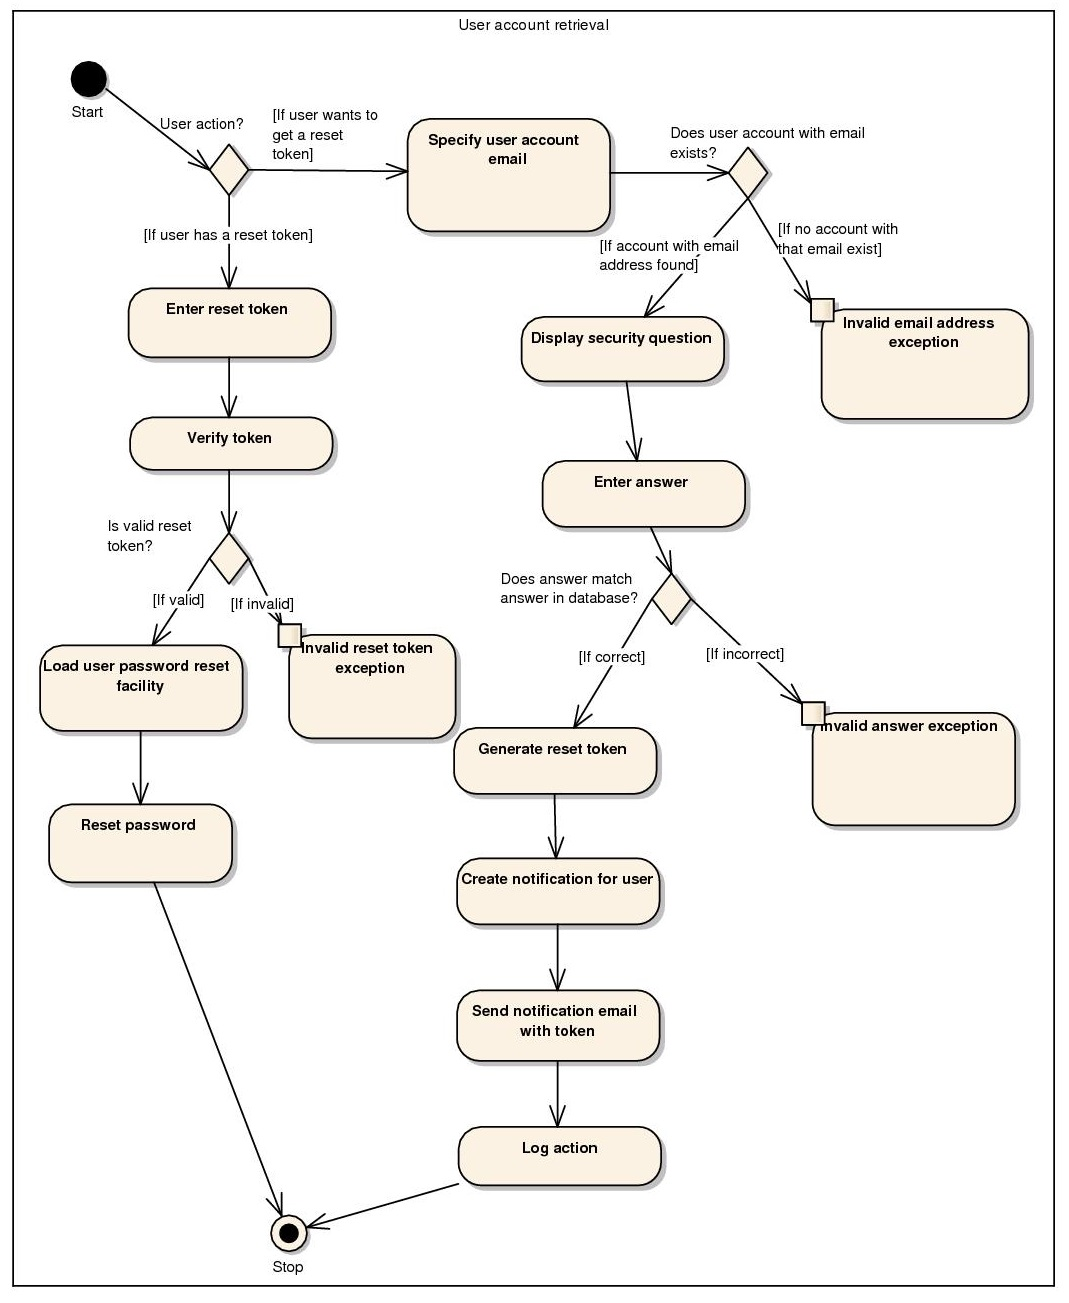
\includegraphics[scale=1]{../Images_Docs/Diagrams/Process specs/User account retrieval.jpg}}
\caption{Activity diagram of the User account retrieval use case.}
\end{figure}

\begin{figure}[H]
\centering	
\framebox{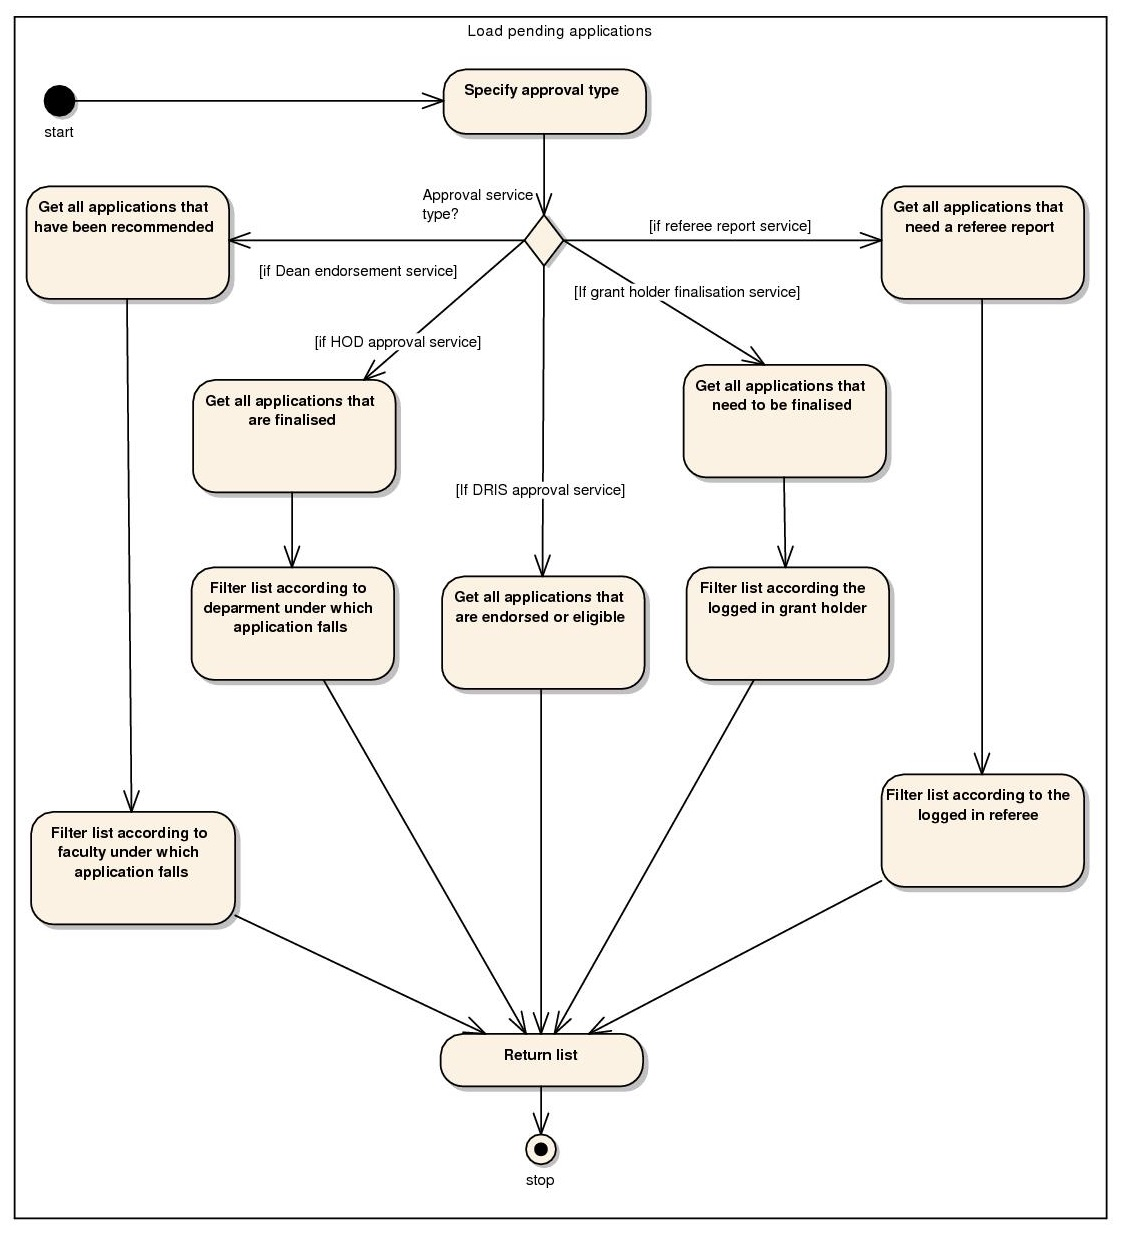
\includegraphics[scale=1]{../Images_Docs/Diagrams/Process specs/Load pending applications.jpg}}
\caption{Activity diagram of the Load pending applications use case.}
\end{figure}

%%%%%%%%%%%%%%%%%%%%%%%%%%%%%%%%%%%%%%%%%%%%%%%%%%%%%%%%%%%%%%%%%%%%%%%%%%%%%%%%%%%%%%%%%%%%%%%%%%%%%%%%%%%%%%%%%%%%%%%%%%%%%%%%%%%%

\begin{figure}[H]
\centering	
\framebox{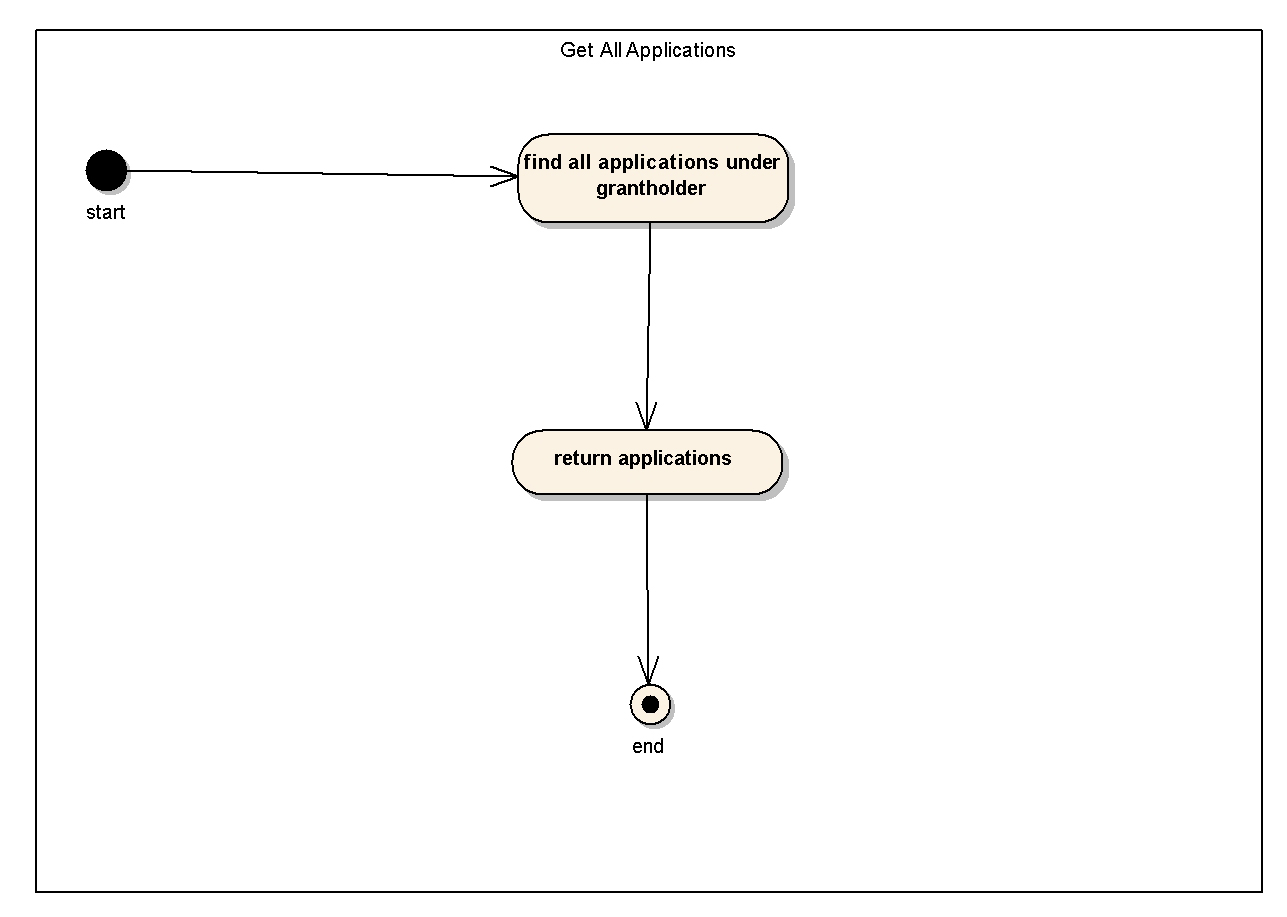
\includegraphics[scale=0.2]{../Images_Docs/Diagrams/Activity Diagrams/ApplicationProgressViewer/Get All Applications.jpg}}
\caption{Activity diagram of the Get All Applications use case.}
\end{figure}

\begin{figure}[H]
\centering	
\framebox{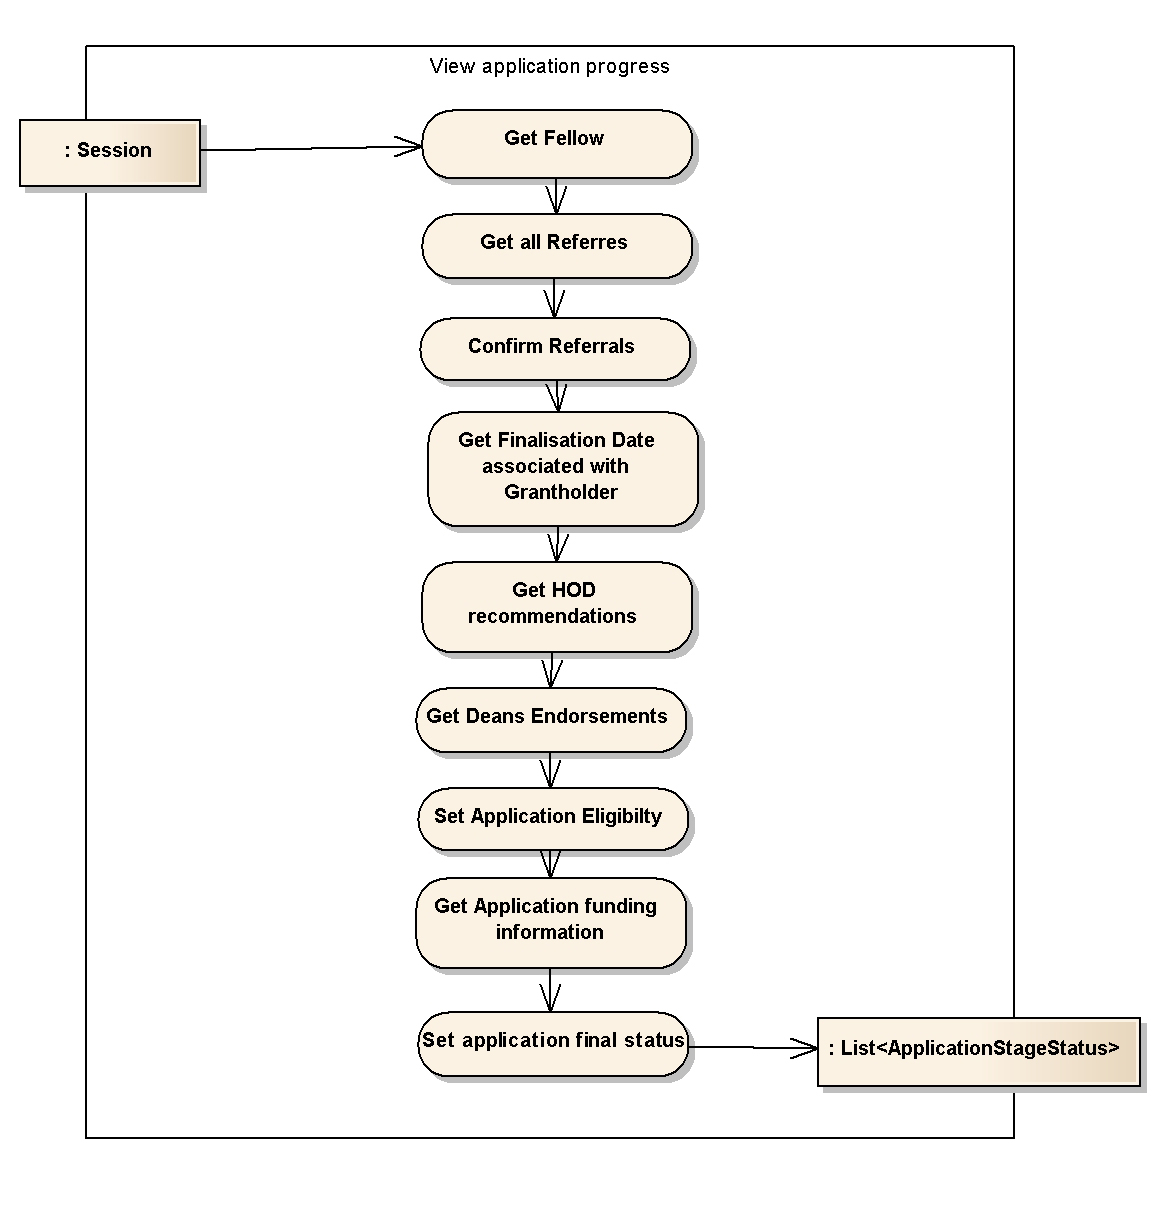
\includegraphics[scale=0.3]{../Images_Docs/Diagrams/Activity Diagrams/ApplicationProgressViewer/View application progress.jpg}}
\caption{Activity diagram of the View application progress use case.}
\end{figure}

%%%%%%%%%%%%%%%%%%%%%%%%%%%%%%%%%%%%%%%%%%%%%%%%%%%%%%%%%%%%%%%%%%%%%%%%%%%%%%%%%%%%%%%%%%%%%%%%%%%%%%%%%%%%%%%%%%%%%%%%%%%%%%%%%%%%

\begin{figure}[H]
\centering	
\framebox{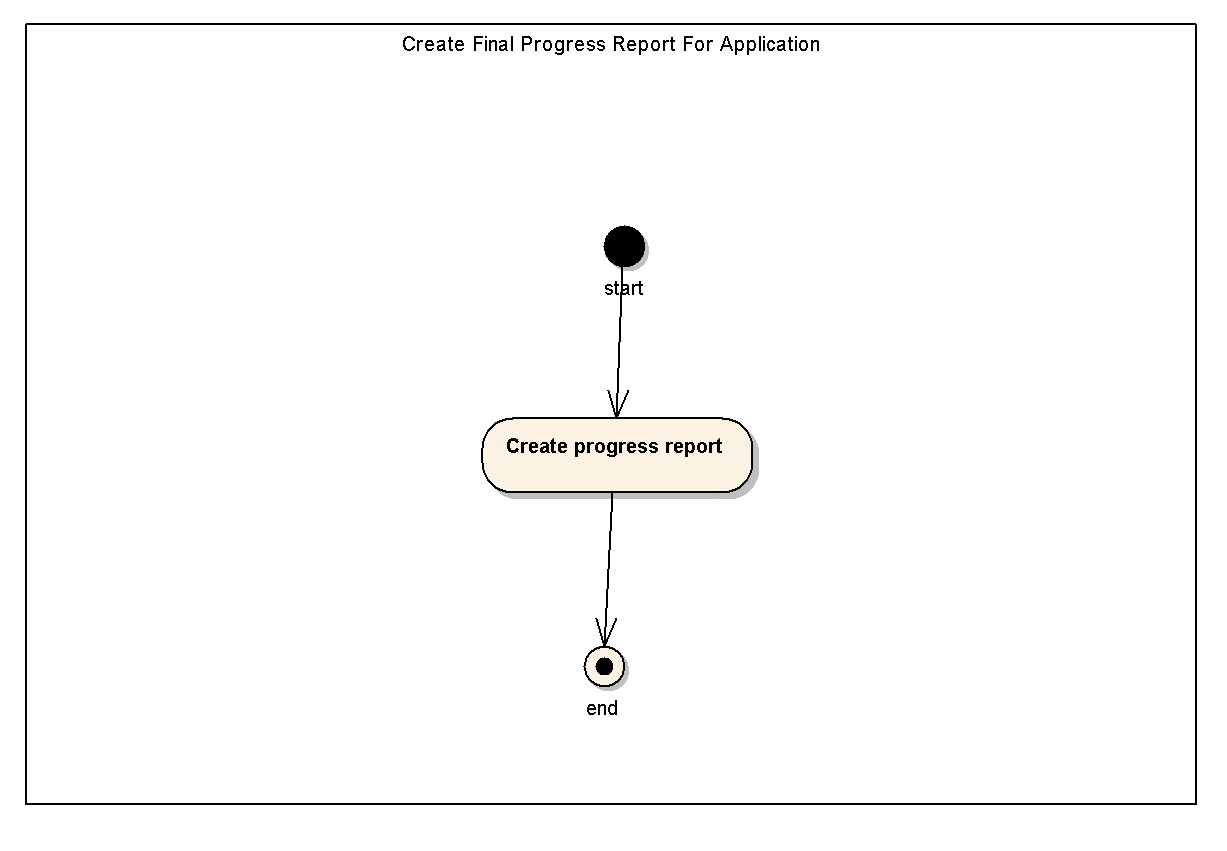
\includegraphics[scale=0.2]{../Images_Docs/Diagrams/Activity Diagrams/ApplicationRenewalService/Create Final Progress Report For Application.jpg}}
\caption{Activity diagram of the Create Final Progress Report For Application use case.}
\end{figure}

\begin{figure}[H]
\centering	
\framebox{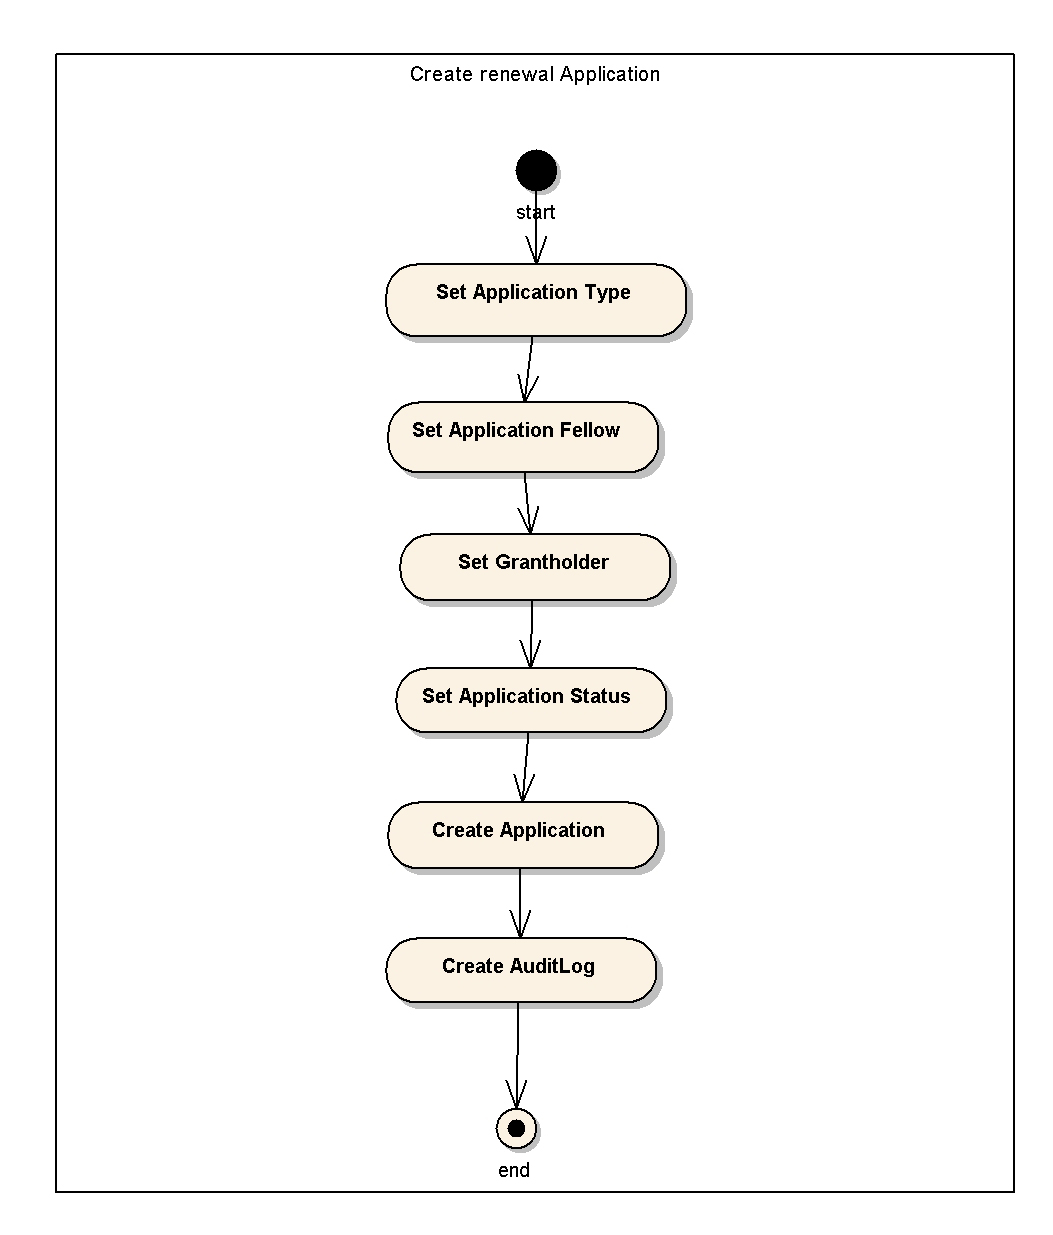
\includegraphics[scale=0.3]{../Images_Docs/Diagrams/Activity Diagrams/ApplicationRenewalService/Create renewal Application.jpg}}
\caption{Activity diagram of the Create renewal Application use case.}
\end{figure}

\begin{figure}[H]
\centering	
\framebox{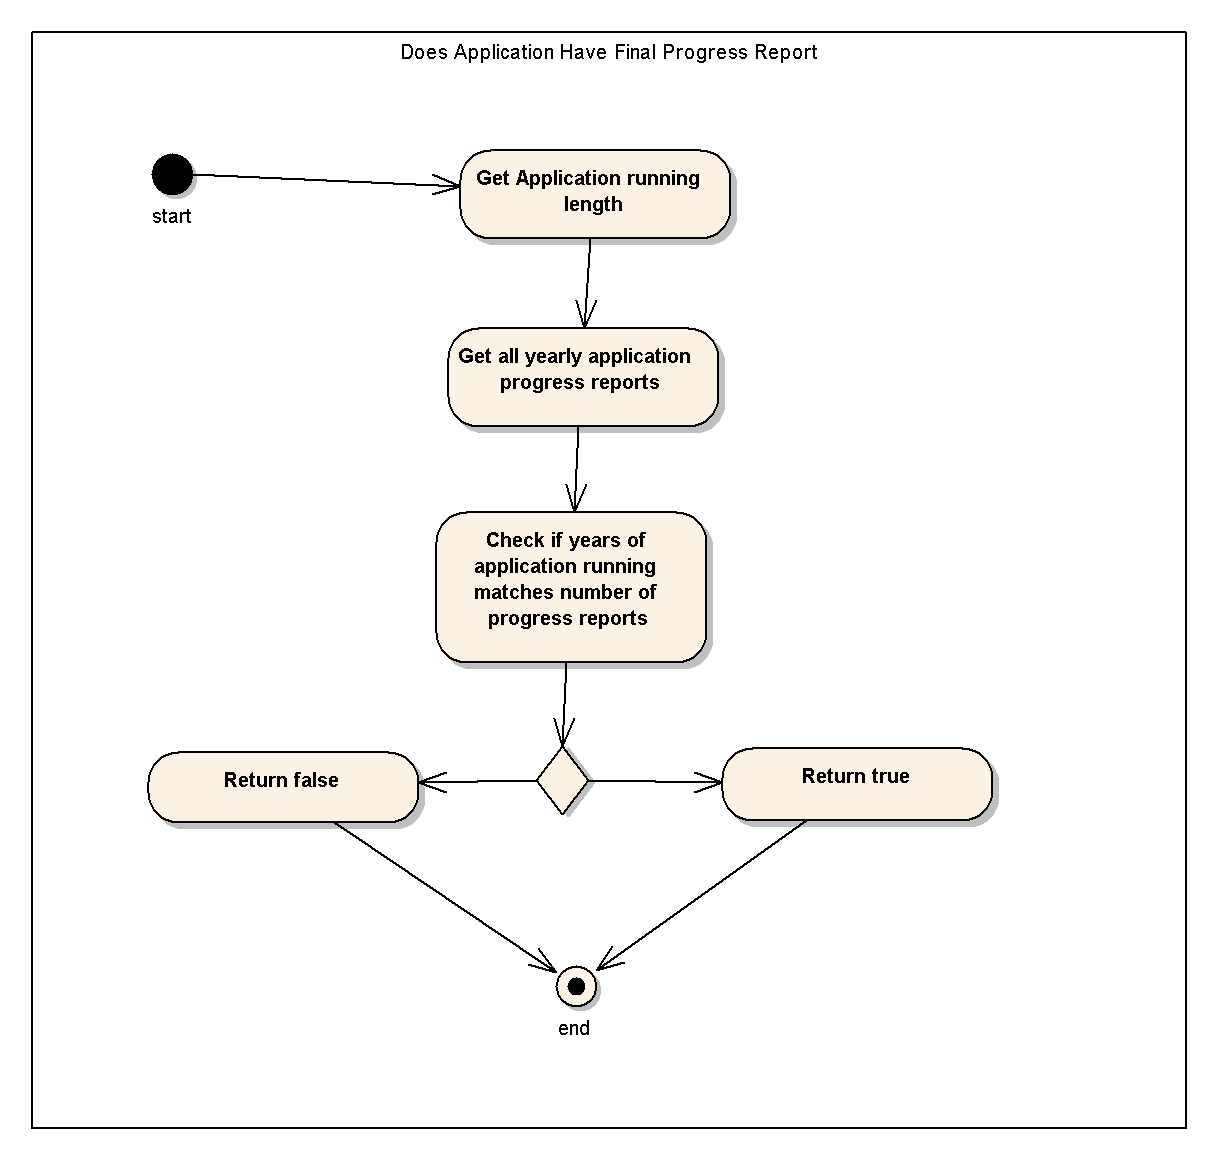
\includegraphics[scale=0.2]{../Images_Docs/Diagrams/Activity Diagrams/ApplicationRenewalService/Does Application Have Final Progress Report.jpg}}
\caption{Activity diagram of the Does Application Have Final Progress Report use case.}
\end{figure}

\begin{figure}[H]
\centering	
\framebox{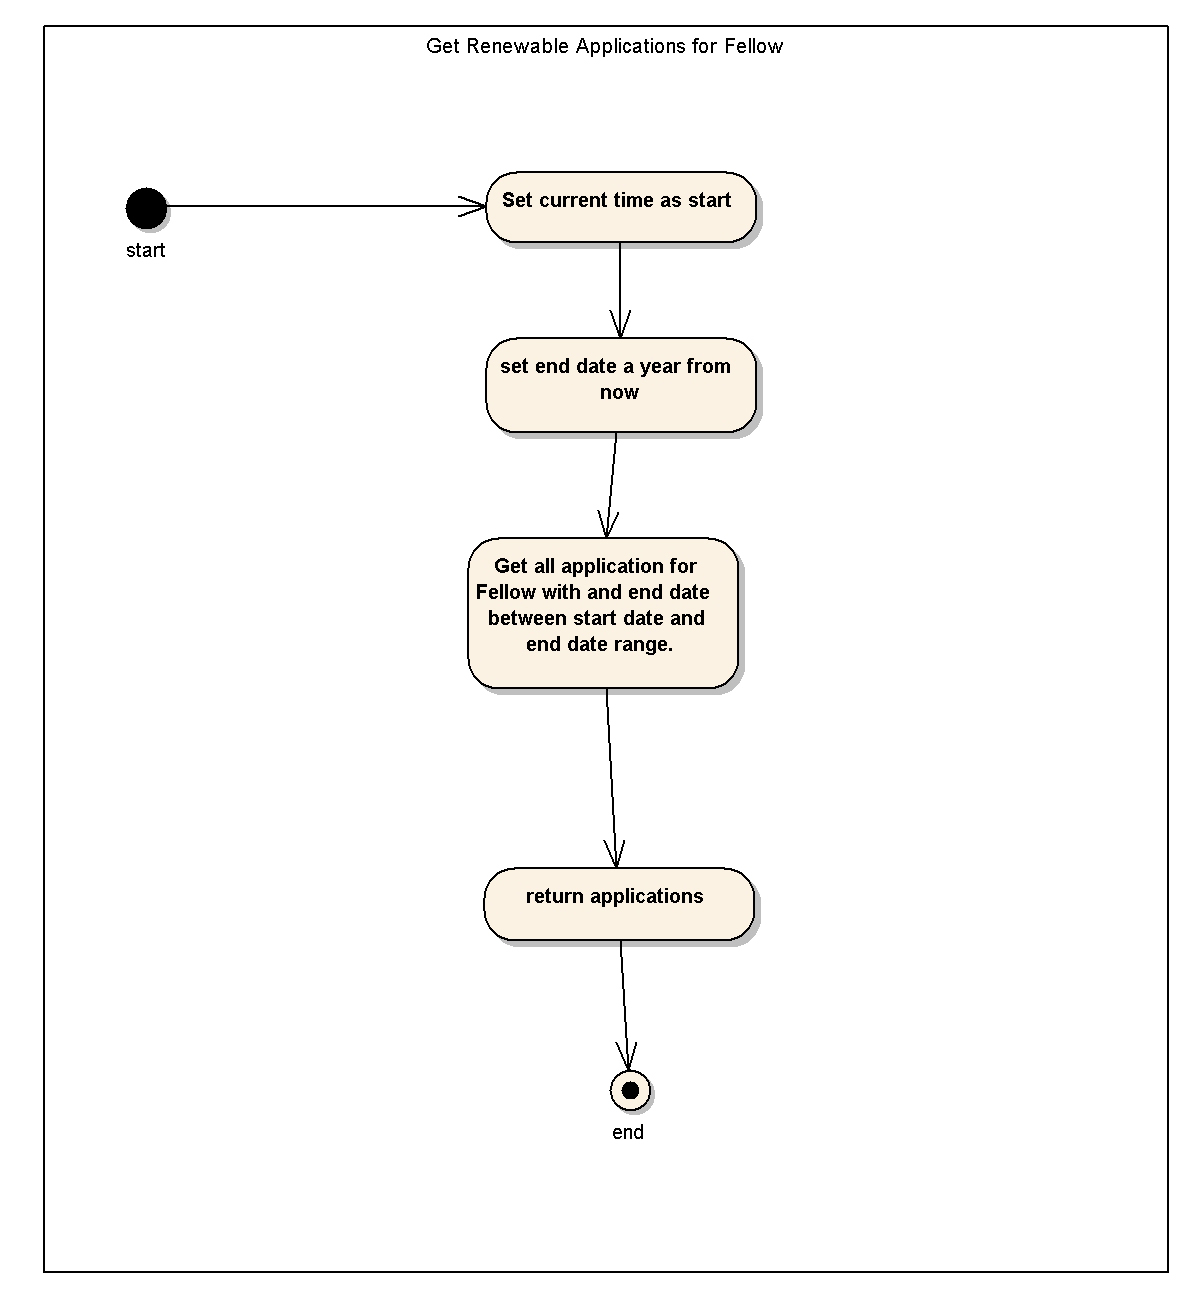
\includegraphics[scale=0.3]{../Images_Docs/Diagrams/Activity Diagrams/ApplicationRenewalService/Get Renewable Applications for Fellow.jpg}}
\caption{Activity diagram of the Get Renewable Applications for Fellow use case.}
\end{figure}

%%%%%%%%%%%%%%%%%%%%%%%%%%%%%%%%%%%%%%%%%%%%%%%%%%%%%%%%%%%%%%%%%%%%%%%%%%%%%%%%%%%%%%%%%%%%%%%%%%%%%%%%%%%%%%%%%%%%%%%%%%%%%%%%%%%%

\begin{figure}[H]
\centering	
\framebox{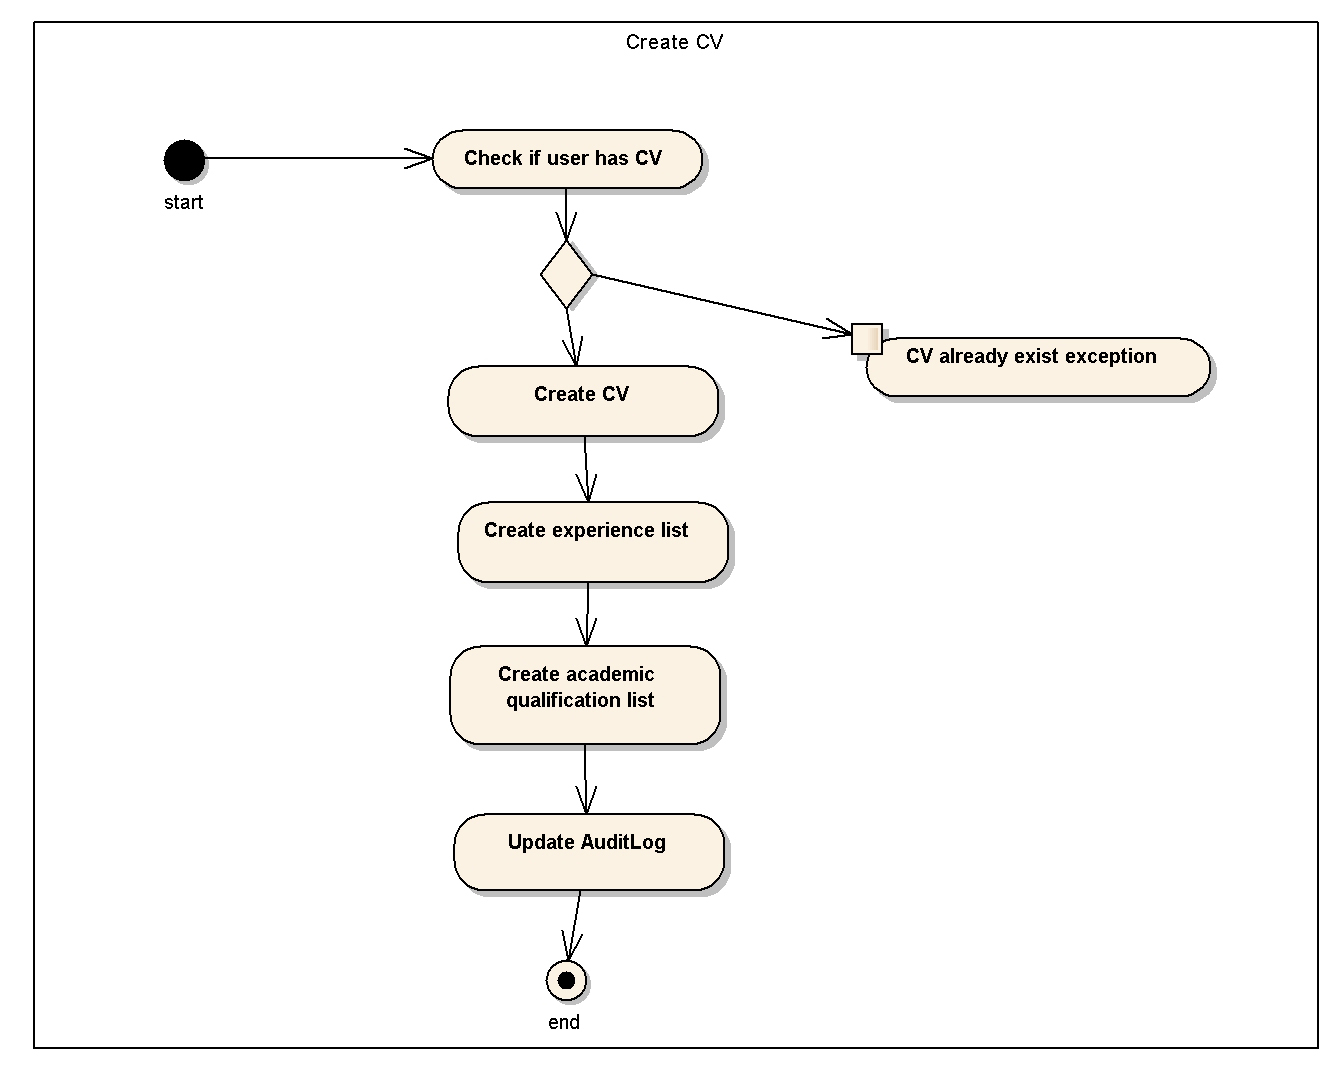
\includegraphics[scale=0.2]{../Images_Docs/Diagrams/Activity Diagrams/CV Management Service/Create CV.jpg}}
\caption{Activity diagram of the Create CV use case.}
\end{figure}

\begin{figure}[H]
\centering	
\framebox{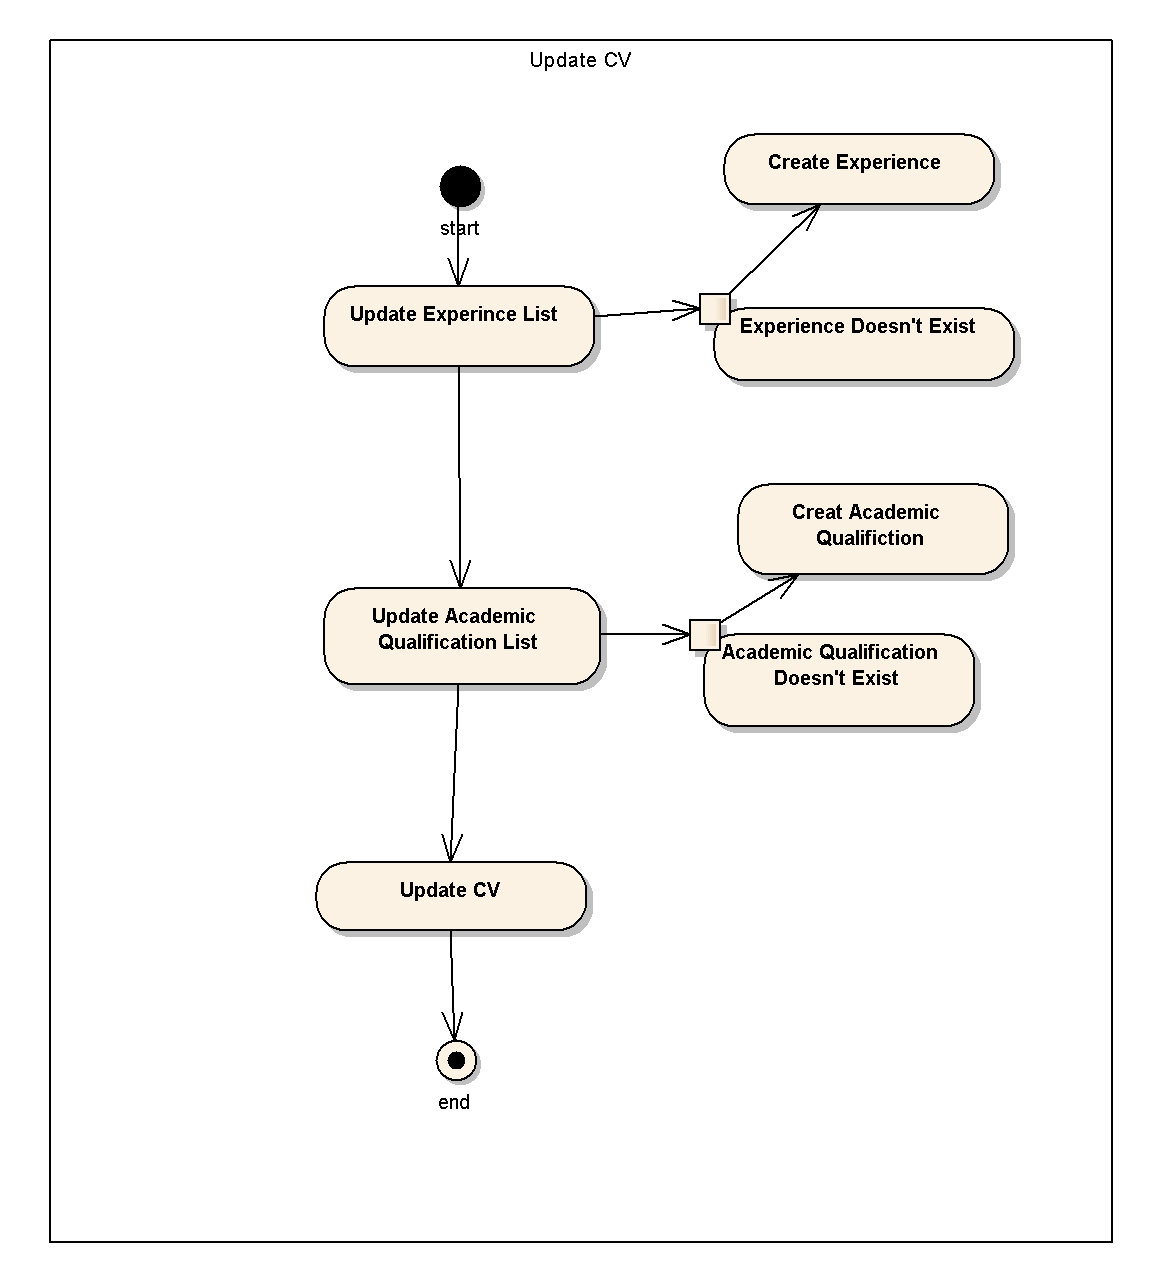
\includegraphics[scale=0.3]{../Images_Docs/Diagrams/Activity Diagrams/CV Management Service/Update CV.jpg}}
\caption{Activity diagram of the Update CV use case.}
\end{figure}

%%%%%%%%%%%%%%%%%%%%%%%%%%%%%%%%%%%%%%%%%%%%%%%%%%%%%%%%%%%%%%%%%%%%%%%%%%%%%%%%%%%%%%%%%%%%%%%%%%%%%%%%%%%%%%%%%%%%%%%%%%%%%%%%%%%%

\begin{figure}[H]
\centering	
\framebox{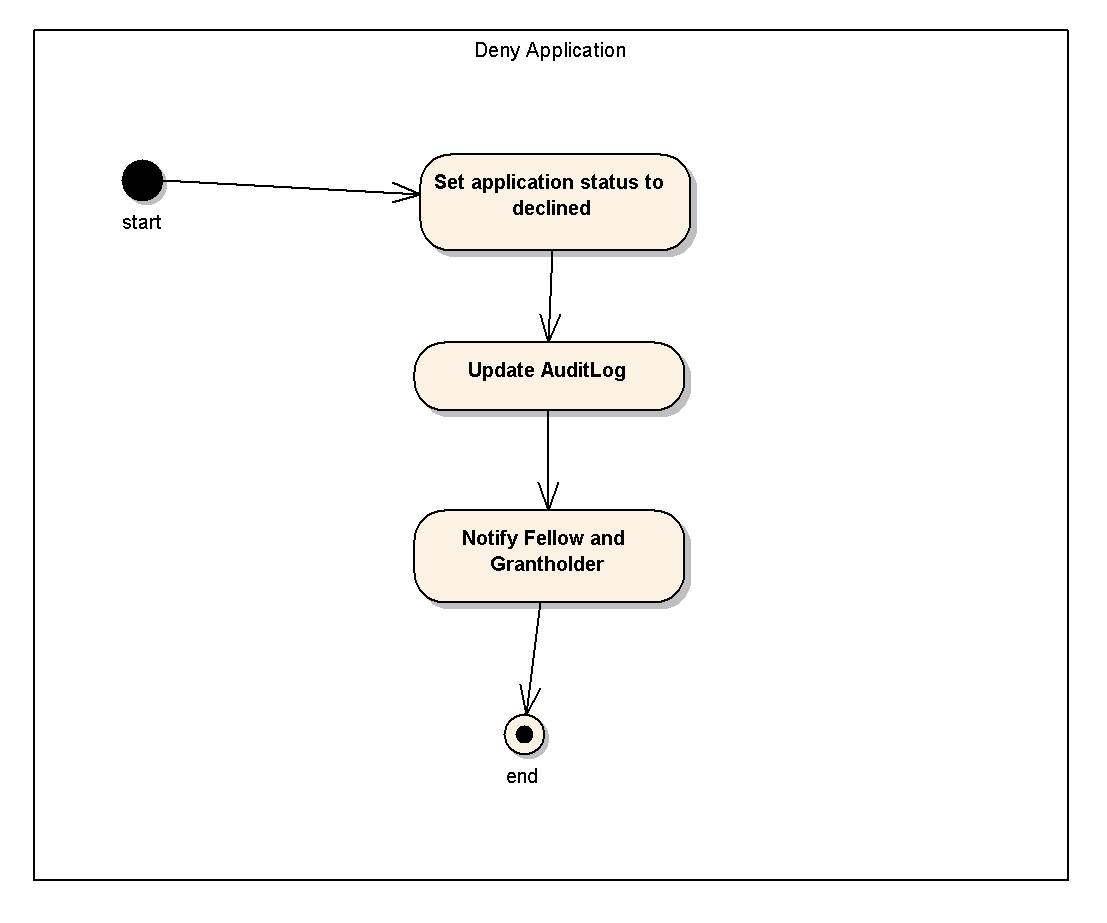
\includegraphics[scale=0.2]{../Images_Docs/Diagrams/Activity Diagrams/Dean Endorsement/Deny Application.jpg}}
\caption{Activity diagram of the Deny Application use case.}
\end{figure}

\begin{figure}[H]
\centering	
\framebox{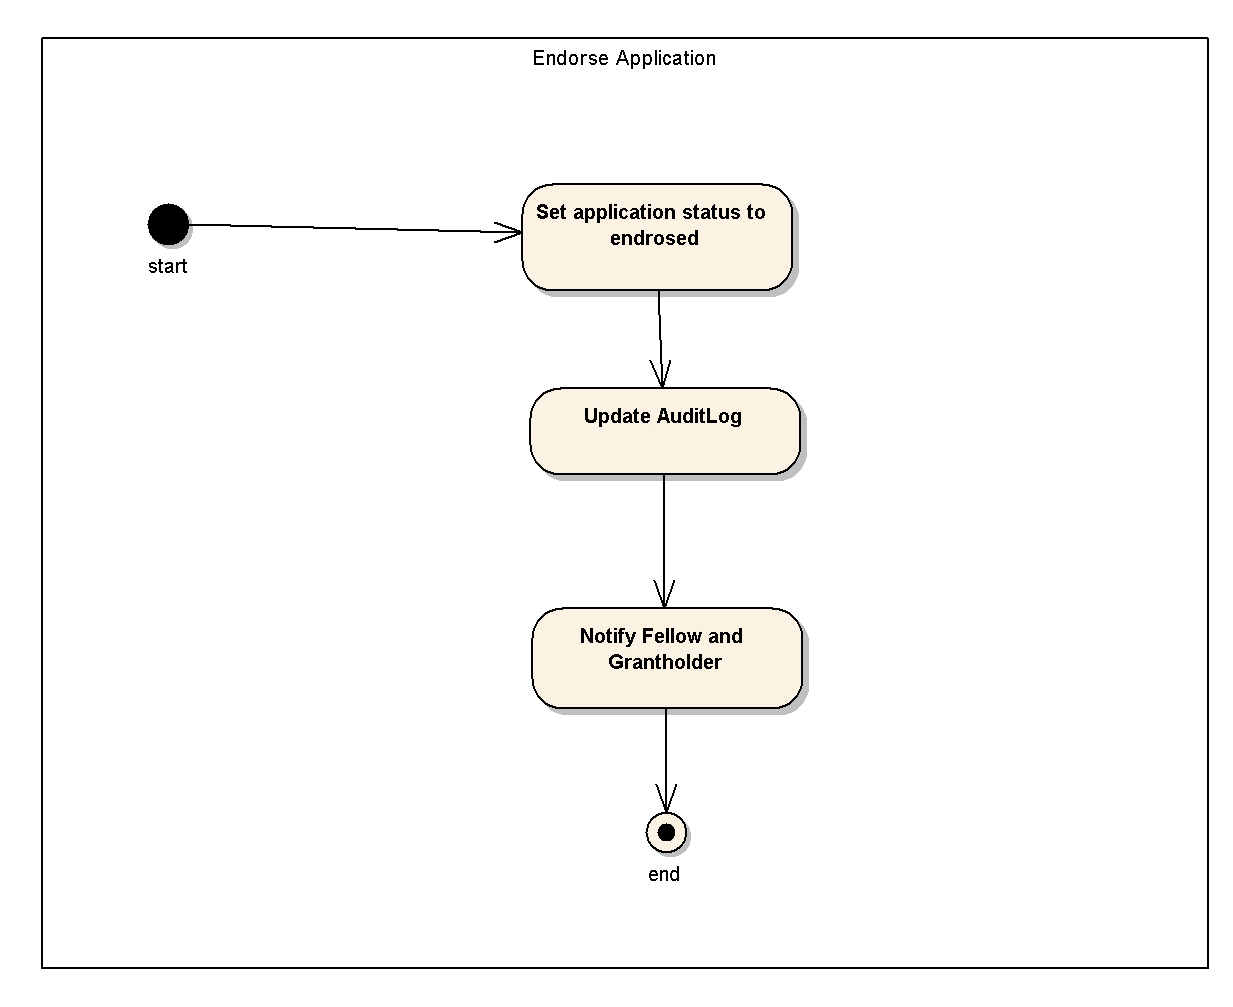
\includegraphics[scale=0.3]{../Images_Docs/Diagrams/Activity Diagrams/Dean Endorsement/Endorse Application.jpg}}
\caption{Activity diagram of the Endorse Application use case.}
\end{figure}

%%%%%%%%%%%%%%%%%%%%%%%%%%%%%%%%%%%%%%%%%%%%%%%%%%%%%%%%%%%%%%%%%%%%%%%%%%%%%%%%%%%%%%%%%%%%%%%%%%%%%%%%%%%%%%%%%%%%%%%%%%%%%%%%%%%%

\begin{figure}[H]
\centering	
\framebox{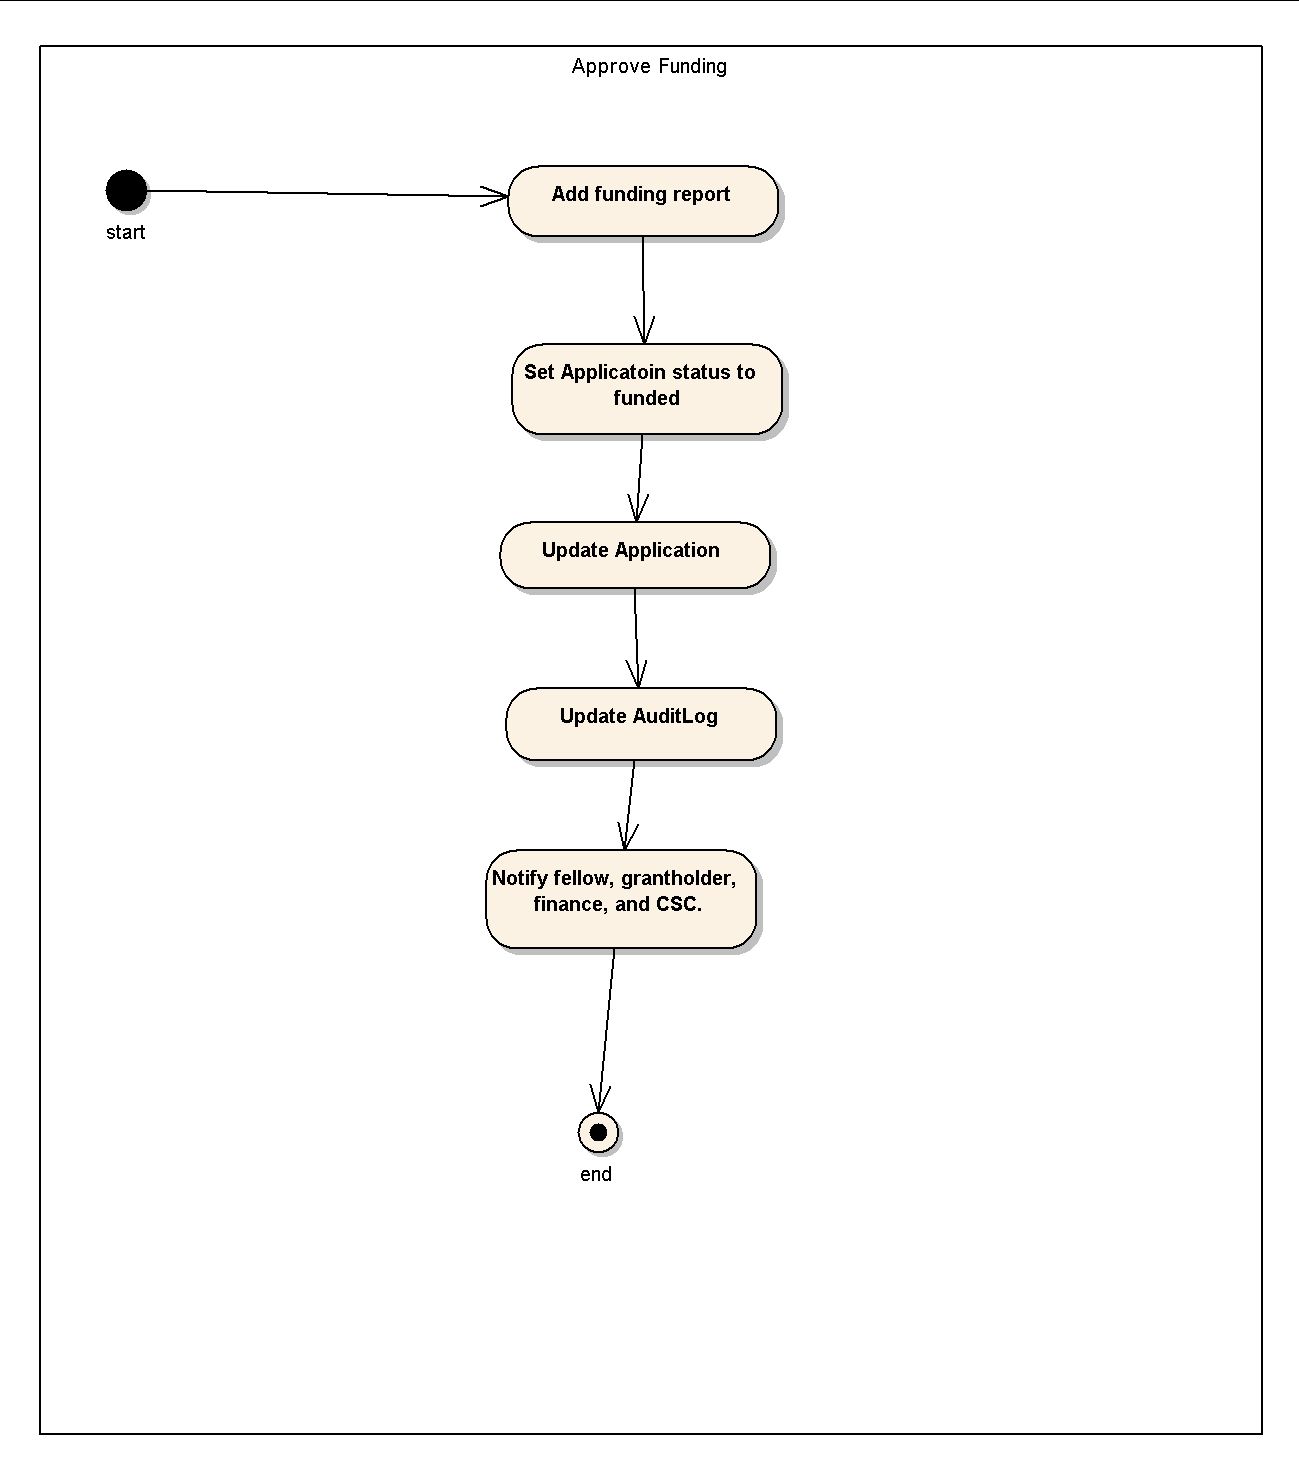
\includegraphics[scale=0.2]{../Images_Docs/Diagrams/Activity Diagrams/DRISApprovalService/Approve Funding.jpg}}
\caption{Activity diagram of the Approve Funding use case.}
\end{figure}

\begin{figure}[H]
\centering	
\framebox{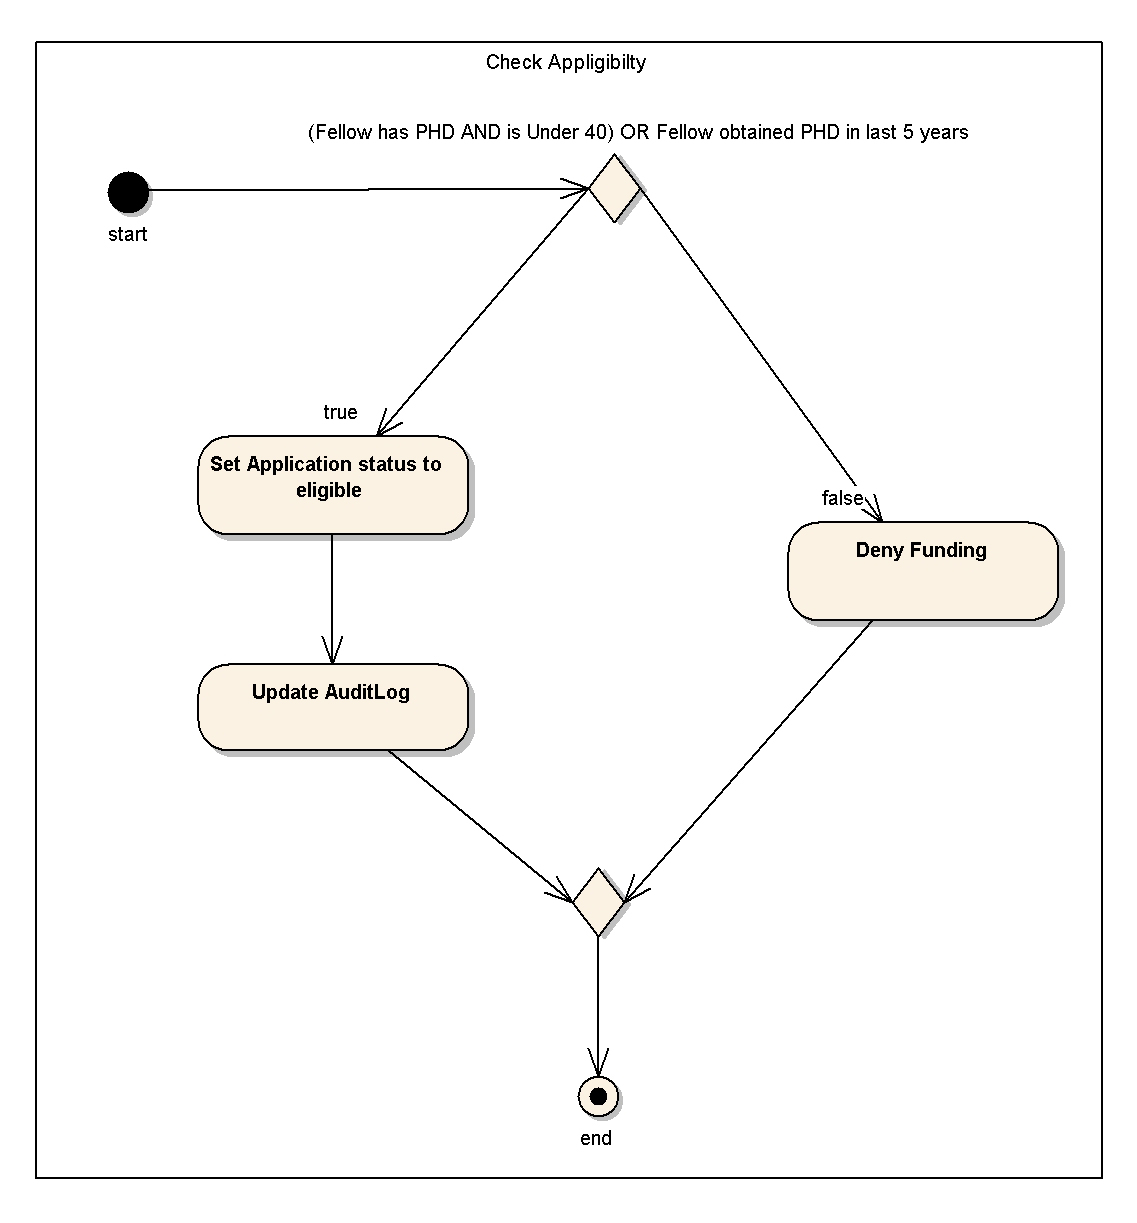
\includegraphics[scale=0.3]{../Images_Docs/Diagrams/Activity Diagrams/DRISApprovalService/Check Appligibilty.jpg}}
\caption{Activity diagram of the Check Appligibilty use case.}
\end{figure}

\begin{figure}[H]
\centering	
\framebox{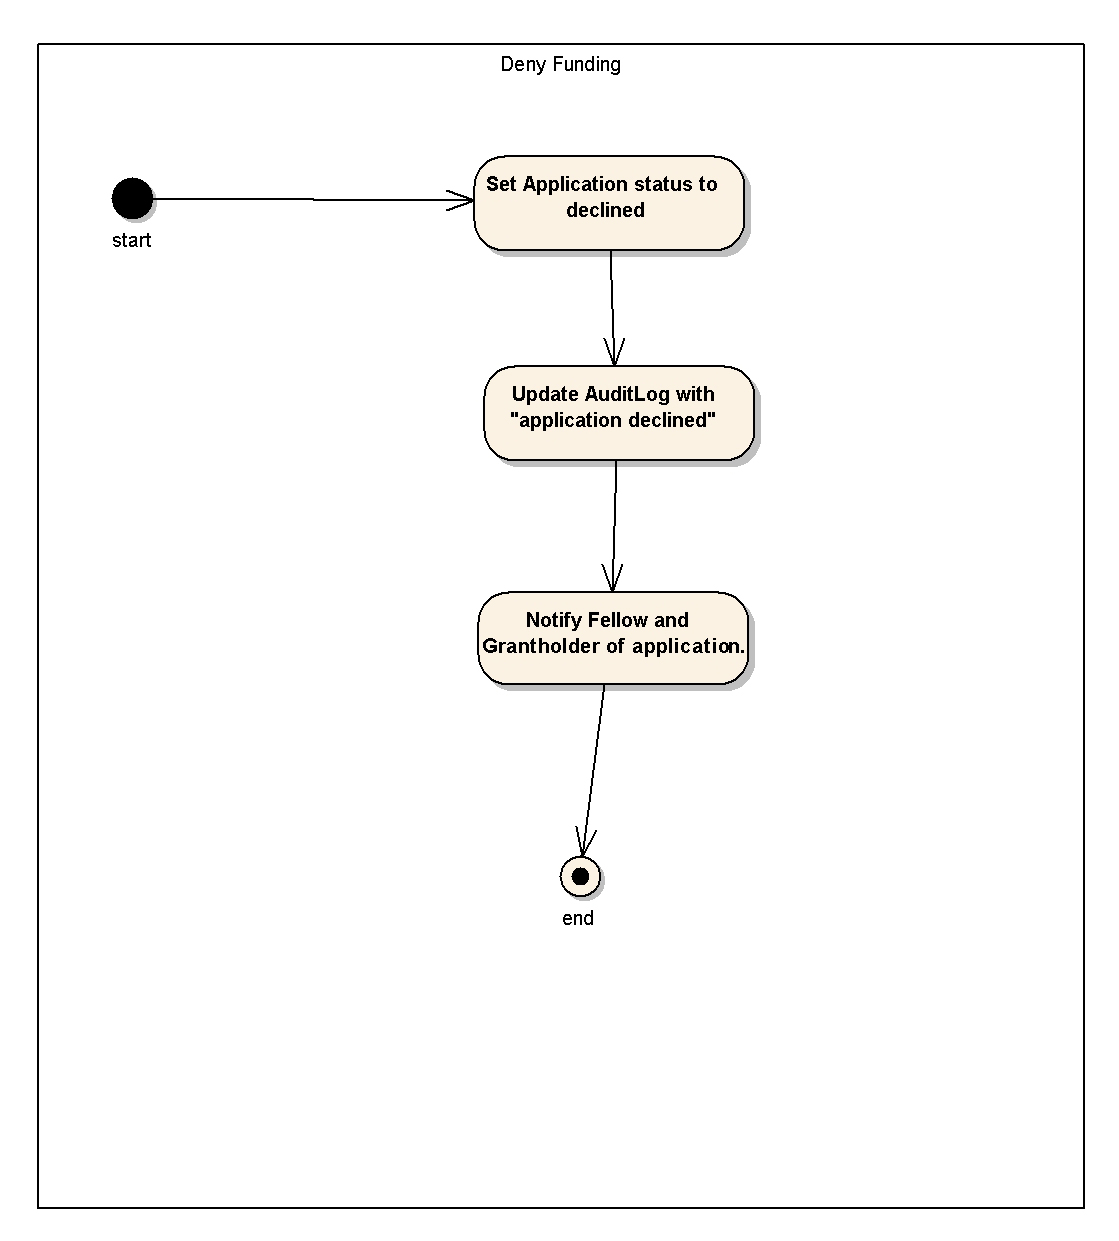
\includegraphics[scale=0.2]{../Images_Docs/Diagrams/Activity Diagrams/DRISApprovalService/Deny Funding.jpg}}
\caption{Activity diagram of the Deny Funding use case.}
\end{figure}

%%%%%%%%%%%%%%%%%%%%%%%%%%%%%%%%%%%%%%%%%%%%%%%%%%%%%%%%%%%%%%%%%%%%%%%%%%%%%%%%%%%%%%%%%%%%%%%%%%%%%%%%%%%%%%%%%%%%%%%%%%%%%%%%%%%%

\begin{figure}[H]
\centering	
\framebox{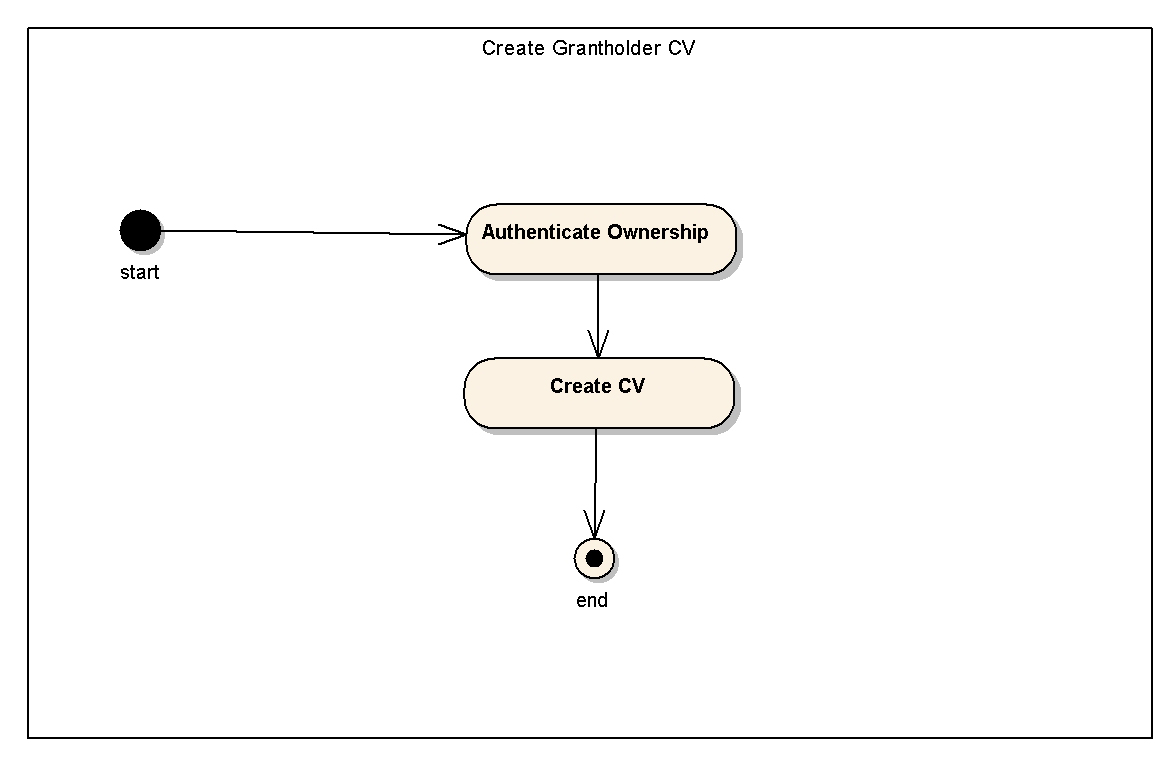
\includegraphics[scale=0.2]{../Images_Docs/Diagrams/Activity Diagrams/GrantHolderFinalisation/Create Grantholder CV.jpg}}
\caption{Activity diagram of the Create Grantholder CV use case.}
\end{figure}

\begin{figure}[H]
\centering	
\framebox{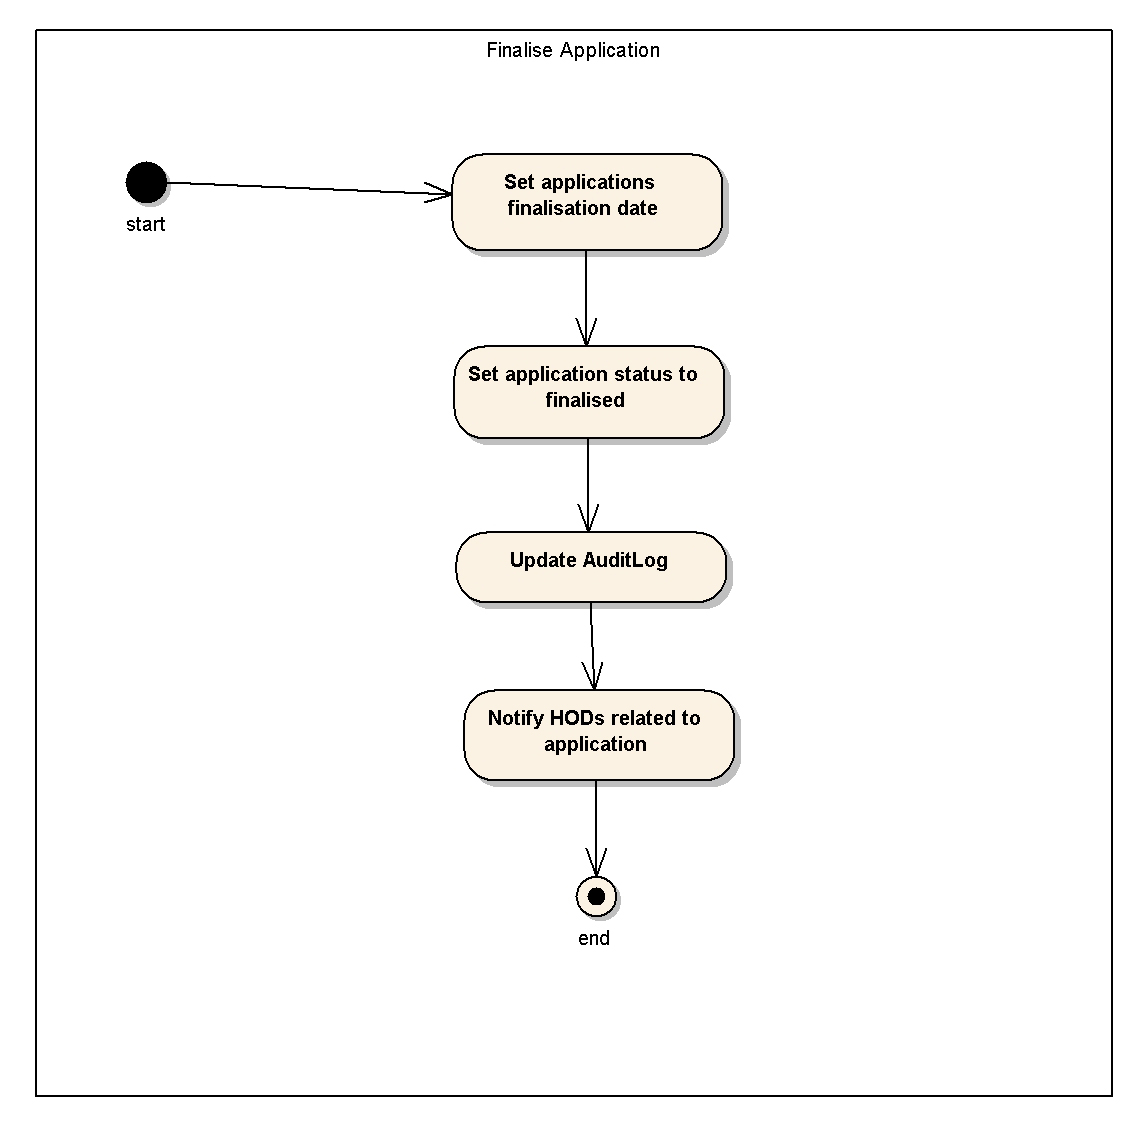
\includegraphics[scale=0.3]{../Images_Docs/Diagrams/Activity Diagrams/GrantHolderFinalisation/Finalise Application.jpg}}
\caption{Activity diagram of the Finalise Application use case.}
\end{figure}

%%%%%%%%%%%%%%%%%%%%%%%%%%%%%%%%%%%%%%%%%%%%%%%%%%%%%%%%%%%%%%%%%%%%%%%%%%%%%%%%%%%%%%%%%%%%%%%%%%%%%%%%%%%%%%%%%%%%%%%%%%%%%%%%%%%%

\begin{figure}[H]
\centering	
\framebox{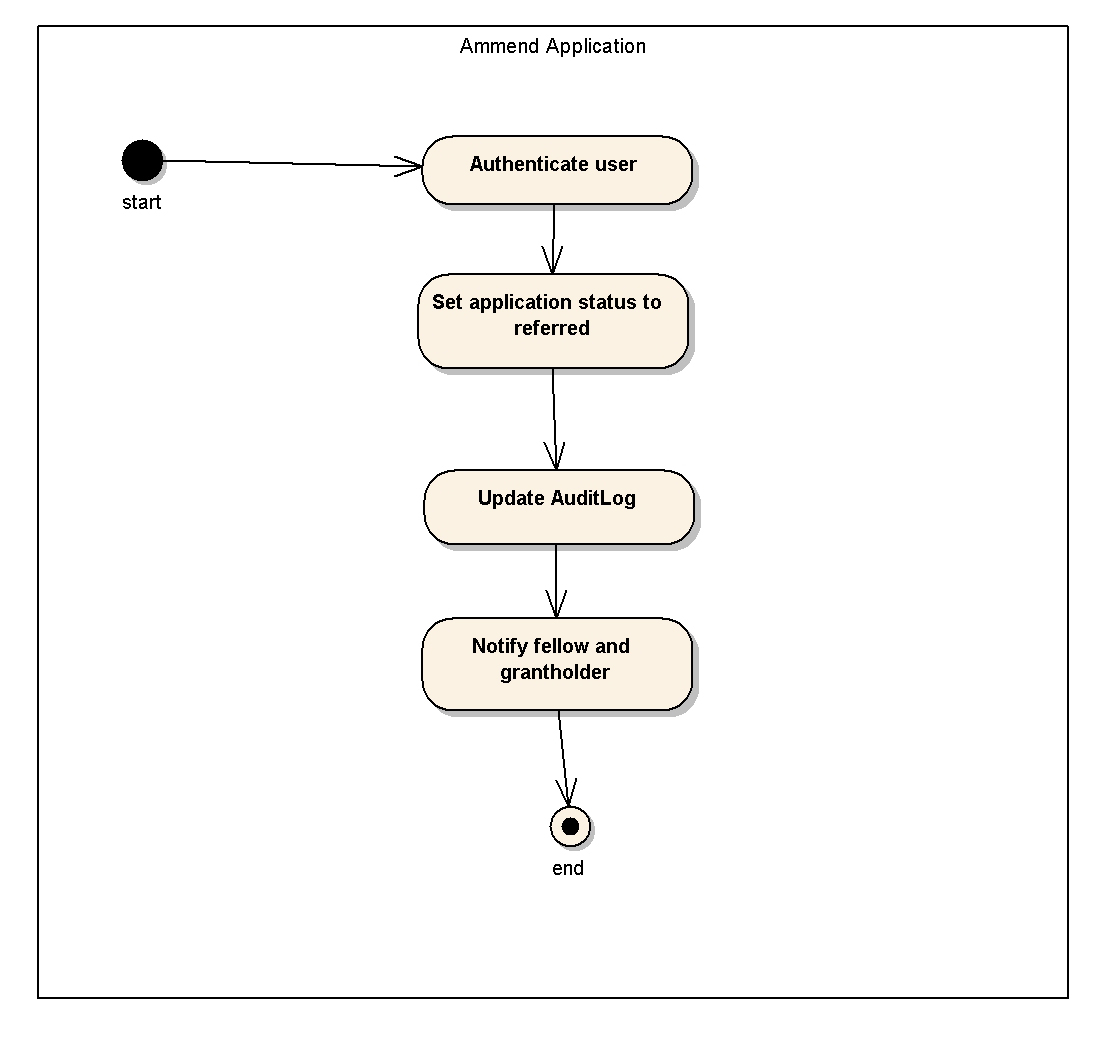
\includegraphics[scale=0.2]{../Images_Docs/Diagrams/Activity Diagrams/HOD recommendations/Ammend Application.jpg}}
\caption{Activity diagram of the Ammend Application use case.}
\end{figure}

\begin{figure}[H]
\centering	
\framebox{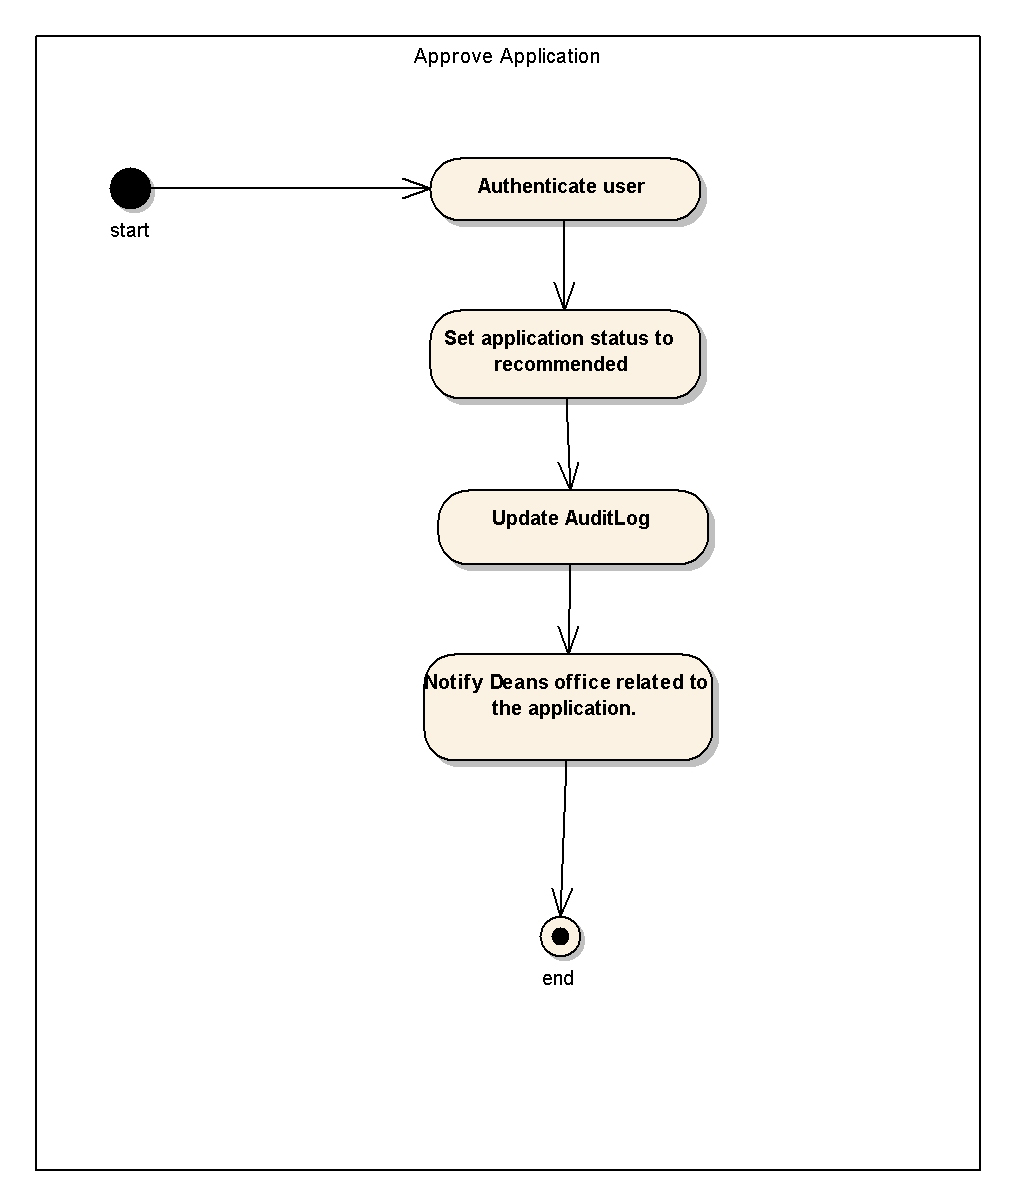
\includegraphics[scale=0.3]{../Images_Docs/Diagrams/Activity Diagrams/HOD recommendations/Approve Application.jpg}}
\caption{Activity diagram of the Approve Application use case.}
\end{figure}

\begin{figure}[H]
\centering	
\framebox{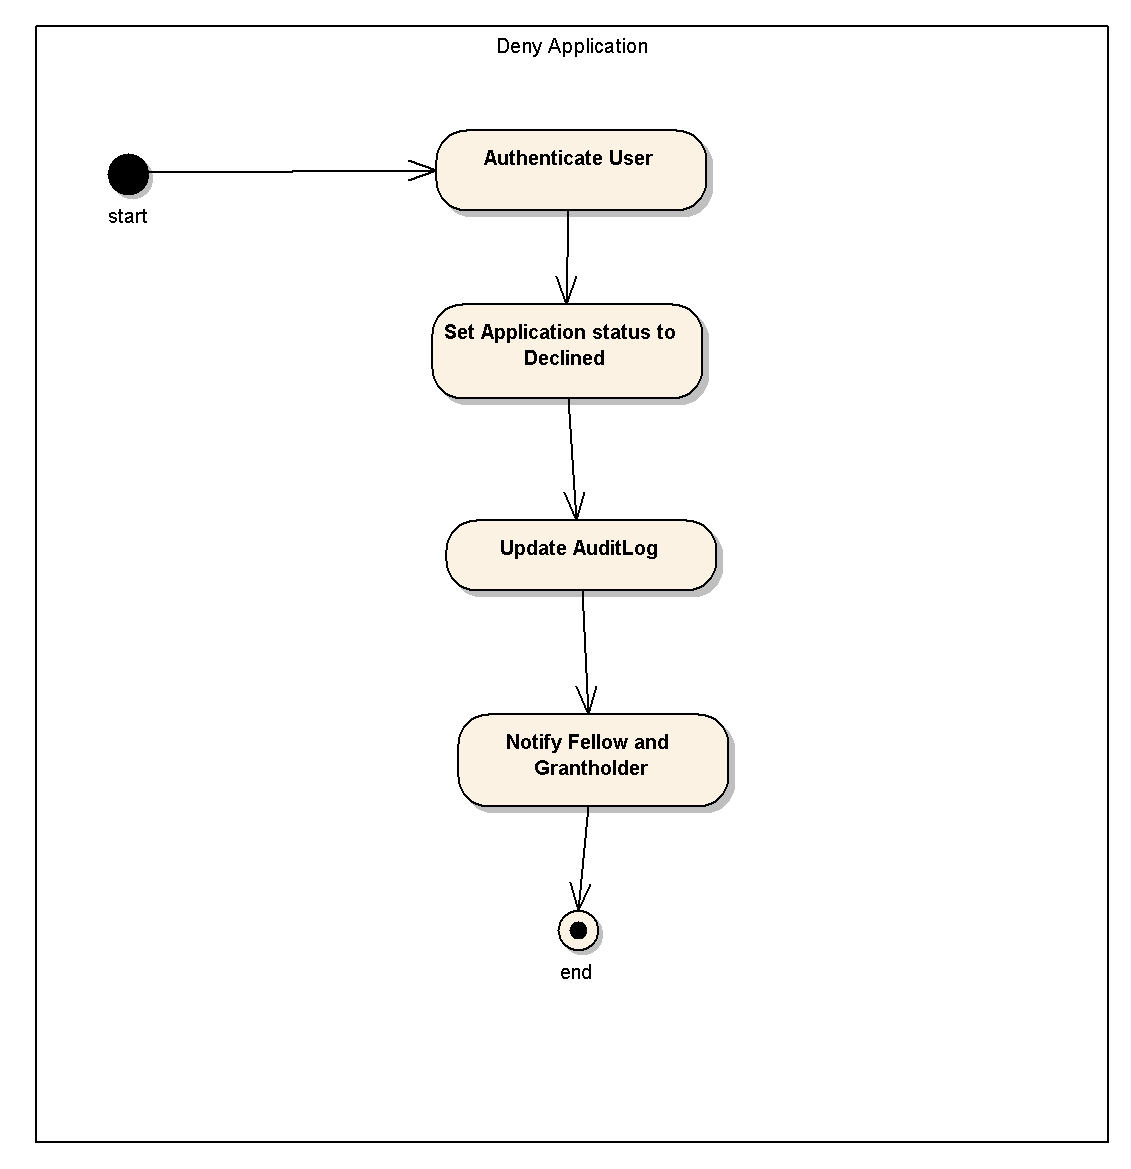
\includegraphics[scale=0.2]{../Images_Docs/Diagrams/Activity Diagrams/HOD recommendations/Deny Application.jpg}}
\caption{Activity diagram of the Deny Application use case.}
\end{figure}

\begin{figure}[H]
\centering	
\framebox{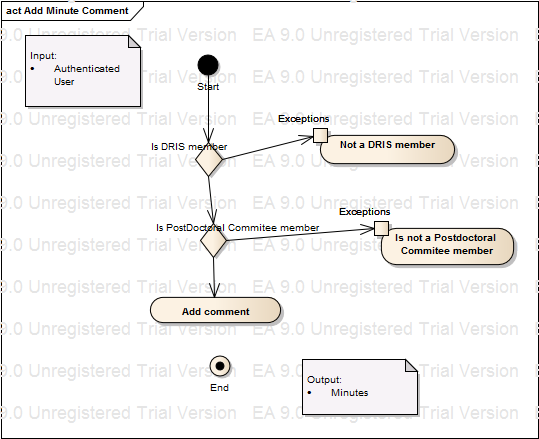
\includegraphics[scale=0.2]{../Images_Docs/Diagrams/Activity Diagrams/MeetingManagement/Add Minute Comment.png}}
\caption{Activity diagram of the Add Minute Comment use case.}
\end{figure}

\begin{figure}[H]
\centering	
\framebox{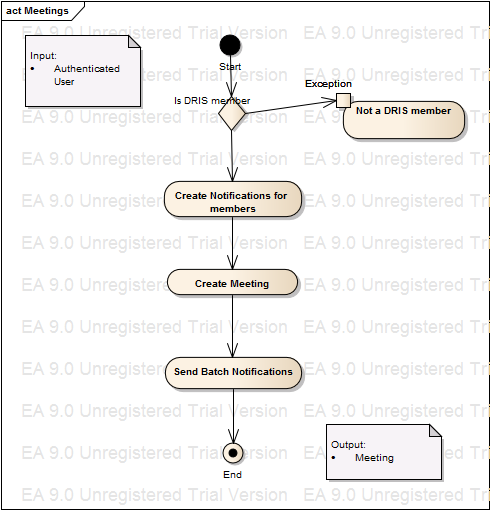
\includegraphics[scale=0.2]{../Images_Docs/Diagrams/Activity Diagrams/MeetingManagement/CreateMeetings.png}}
\caption{Activity diagram of the Create Meeting use case.}
\end{figure}

\begin{figure}[H]
\centering	
\framebox{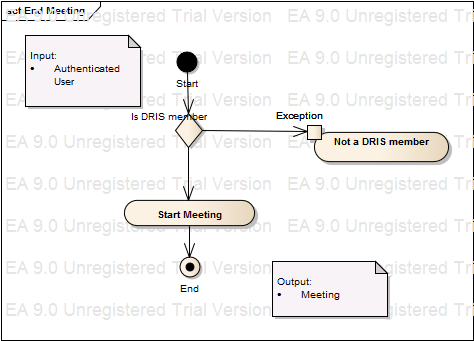
\includegraphics[scale=0.2]{../Images_Docs/Diagrams/Activity Diagrams/MeetingManagement/EndMeeting.png}}
\caption{Activity diagram of the End Meeting use case.}
\end{figure}

\begin{figure}[H]
\centering	
\framebox{\includegraphics[scale=0.2]{../Images_Docs/Diagrams/Activity Diagrams/MeetingManagement/GetAllActiveMeeting.png}}
\caption{Activity diagram of the Get All Active Meetings use case.}
\end{figure}

\begin{figure}[H]
\centering	
\framebox{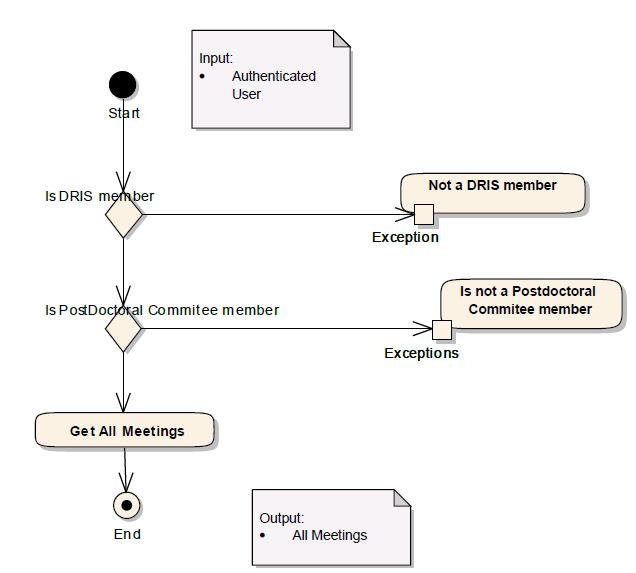
\includegraphics[scale=0.2]{../Images_Docs/Diagrams/Activity Diagrams/MeetingManagement/GetAllMeetings.png}}
\caption{Activity diagram of the Get All Meetings use case.}
\end{figure}


\begin{figure}[H]
\centering	
\framebox{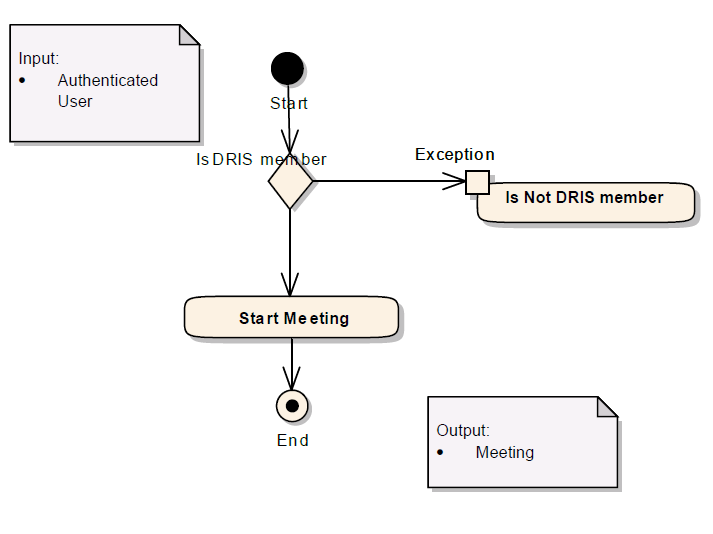
\includegraphics[scale=0.2]{../Images_Docs/Diagrams/Activity Diagrams/MeetingManagement/StartMeeting.png}}
\caption{Activity diagram of the Start Meeting use case.}
\end{figure}

\begin{figure}[H]
\centering	
\framebox{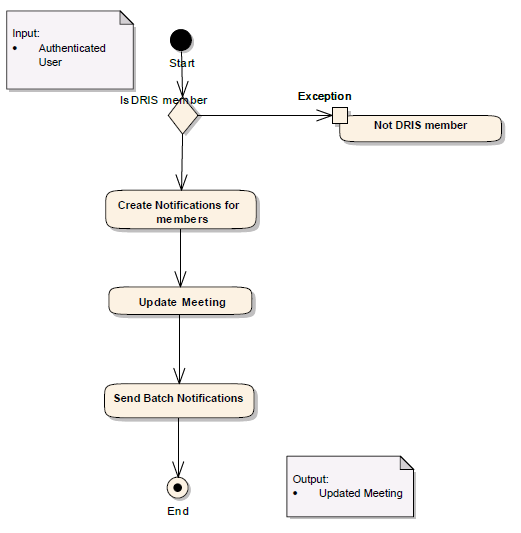
\includegraphics[scale=0.2]{../Images_Docs/Diagrams/Activity Diagrams/MeetingManagement/UpdateMeeting.png}}
\caption{Activity diagram of the Update Meeting use case.}
\end{figure}

\begin{figure}[H]
\centering	
\framebox{\includegraphics[scale=0.2]{../Images_Docs/Diagrams/Activity Diagrams/NewApplication/CanFellowOpenNewApplication.png}}
\caption{Activity diagram of the Can the fellow open a New Application use case.}
\end{figure}

\begin{figure}[H]
\centering	
\framebox{\includegraphics[scale=0.2]{../Images_Docs/Diagrams/Activity Diagrams/NewApplication/CreateCV.png}}
\caption{Activity diagram of the Create CV use case.}
\end{figure}

\begin{figure}[H]
\centering	
\framebox{\includegraphics[scale=0.2]{../Images_Docs/Diagrams/Activity Diagrams/NewApplication/CreateNewApplication.png}}
\caption{Activity diagram of the Create New Application use case.}
\end{figure}

\begin{figure}[H]
\centering	
\framebox{\includegraphics[scale=0.2]{../Images_Docs/Diagrams/Activity Diagrams/NewApplication/CreateCV.png}}
\caption{Activity diagram of the Get Open Application use case.}
\end{figure}

\begin{figure}[H]
\centering	
\framebox{\includegraphics[scale=0.2]{../Images_Docs/Diagrams/Activity Diagrams/NewApplication/LinkGrantHolderToApplication.png}}
\caption{Activity diagram of the Link Grant Holder to Application use case.}
\end{figure}

\begin{figure}[H]
\centering	
\framebox{\includegraphics[scale=0.2]{../Images_Docs/Diagrams/Activity Diagrams/NewApplication/LinkRefereeToApplication.png}}
\caption{Activity diagram of the Link Referee to Application use case.}
\end{figure}

\begin{figure}[H]
\centering	
\framebox{\includegraphics[scale=0.2]{../Images_Docs/Diagrams/Activity Diagrams/NewApplication/SubmitApplication.png}}
\caption{Activity diagram of the Submit Application use case.}
\end{figure}

\begin{figure}[H]
\centering	
\framebox{\includegraphics[scale=0.2]{../Images_Docs/Diagrams/Activity Diagrams/Notifications/GetNotificationsForPerson.png}}
\caption{Activity diagram of the Get Notifications for Person use case.}
\end{figure}


\begin{figure}[H]
\centering	
\framebox{\includegraphics[scale=0.2]{../Images_Docs/Diagrams/Activity Diagrams/Notifications/GetNotificationsFromPerson.png}}
\caption{Activity diagram of the Get Notifications from Person use case.}
\end{figure}


\begin{figure}[H]
\centering	
\framebox{\includegraphics[scale=0.2]{../Images_Docs/Diagrams/Activity Diagrams/Notifications/SendBatchNotifications.png}}
\caption{Activity diagram of the Send batch Notifications use case.}
\end{figure}


\begin{figure}[H]
\centering	
\framebox{\includegraphics[scale=0.2]{../Images_Docs/Diagrams/Activity Diagrams/ProgressReportManagement/CreateProgressReport.png}}
\caption{Activity diagram of the Create Progress Report use case.}
\end{figure}

\begin{figure}[H]
\centering	
\framebox{\includegraphics[scale=0.2]{../Images_Docs/Diagrams/Activity Diagrams/ProgressReportManagement/UpdateProgressReport.png}}
\caption{Activity diagram of the Update Progress Report use case.}
\end{figure}

\begin{figure}[H]
\centering	
\framebox{\includegraphics[scale=0.2]{../Images_Docs/Diagrams/Activity Diagrams/RefereeReport/RefereesReport.png}}
\caption{Activity diagram of the Create Referee Report use case.}
\end{figure}

\begin{figure}[H]
\centering	
\framebox{\includegraphics[scale=0.2]{../Images_Docs/Diagrams/Activity Diagrams/RefereeReport/SubmitReferralReport.png}}
\caption{Activity diagram of the Submit Referee Report use case.}
\end{figure}

\begin{figure}[H]
\centering	
\framebox{\includegraphics[scale=0.2]{../Images_Docs/Diagrams/Activity Diagrams/RefereeReport/CountPendingApplications.png}}
\caption{Activity diagram of the Count Pending Reports use case.}
\end{figure}

\begin{figure}[H]
\centering	
\framebox{\includegraphics[scale=0.2]{../Images_Docs/Diagrams/Activity Diagrams/Reporting/ExportPDF.png}}
\caption{Activity diagram of the Export PDF Report use case.}
\end{figure}

\begin{figure}[H]
\centering	
\framebox{\includegraphics[scale=0.2]{../Images_Docs/Diagrams/Activity Diagrams/Reporting/ExportApplicationSpreadsheet.png}}
\caption{Activity diagram of the Export PDF Report use case.}
\end{figure}


\begin{figure}[H]
\centering	
\framebox{\includegraphics[scale=0.2]{../Images_Docs/Diagrams/Activity Diagrams/UserAccountManagement/GenerateSystemID.png}}
\caption{Activity diagram of the Generate System ID use case.}
\end{figure}

\begin{figure}[H]
\centering	
\framebox{\includegraphics[scale=0.2]{../Images_Docs/Diagrams/Activity Diagrams/UserAccountManagement/GetAllSecurityRoles.png}}
\caption{Activity diagram of the Get All Security Roles use case.}
\end{figure}

\begin{figure}[H]
\centering	
\framebox{\includegraphics[scale=0.2]{../Images_Docs/Diagrams/Activity Diagrams/UserAccountManagement/GetUserByEmail.png}}
\caption{Activity diagram of the Get user by Email use case.}
\end{figure}

\begin{figure}[H]
\centering	
\framebox{\includegraphics[scale=0.2]{../Images_Docs/Diagrams/Activity Diagrams/UserAccountManagement/GetUserbySystem ID.png}}
\caption{Activity diagram of the Get User by System ID use case.}
\end{figure}

\begin{figure}[H]
\centering	
\framebox{\includegraphics[scale=0.2]{../Images_Docs/Diagrams/Activity Diagrams/UserAccountManagement/RemoveUser.png}}
\caption{Activity diagram of the Remove User use case.}
\end{figure}

\begin{figure}[H]
\centering	
\framebox{\includegraphics[scale=0.2]{../Images_Docs/Diagrams/Activity Diagrams/UserAccountManagement/UpdateUserAccount.png}}
\caption{Activity diagram of the Update User use case.}
\end{figure}

\begin{figure}[H]
\centering	
\framebox{\includegraphics[scale=0.2]{../Images_Docs/Diagrams/Activity Diagrams/UserAccountManagement/ViewAllAccounts.png}}
\caption{Activity diagram of the View All Users use case.}
\end{figure}

\begin{figure}[H]
\centering	
\framebox{\includegraphics[scale=0.2]{../Images_Docs/Diagrams/Activity Diagrams/UserGateway/AuthenticateUserAsOwner.png}}
\caption{Activity diagram of the Authenticate User as Owner use case.}
\end{figure}

\begin{figure}[H]
\centering	
\framebox{\includegraphics[scale=0.2]{../Images_Docs/Diagrams/Activity Diagrams/UserGateway/GetSessionFromHttpSession.png}}
\caption{Activity diagram of the Get Http Session from Session use case.}
\end{figure}


\begin{figure}[H]
\centering	
\framebox{\includegraphics[scale=0.2]{../Images_Docs/Diagrams/Activity Diagrams/UserGateway/Logout.png}}
\caption{Activity diagram of the Logout use case.}
\end{figure}

\vspace{0.2in}
\newpage

\subsection{Interface Diagrams}

\begin{figure}[H]
\centering	
\framebox{\includegraphics[scale=0.5]{../Images_Docs/Diagrams/Interface Diagram/ApplicationProgressViewerService.jpg}}
\caption{Interface Diagram for the Application Progress Viewer service.}
\end{figure}

\begin{figure}[H]
\centering	
\framebox{\includegraphics[scale=0.5]{../Images_Docs/Diagrams/Interface Diagram/ApplicationRenewalService.jpg}}
\caption{Interface Diagram for the Application Renewal service.}
\end{figure}

\begin{figure}[H]
\centering	
\framebox{\includegraphics[scale=0.5]{../Images_Docs/Diagrams/Interface Diagram/ArchivalService.jpg}}
\caption{Interface Diagram for the Archival service.}
\end{figure}

\begin{figure}[H]
\centering	
\framebox{\includegraphics[scale=0.5]{../Images_Docs/Diagrams/Interface Diagram/CVManagementService.jpg}}
\caption{Interface Diagram for the CV Management service.}
\end{figure}


\begin{figure}[H]
\centering	
\framebox{\includegraphics[scale=0.5]{../Images_Docs/Diagrams/Interface Diagram/DeansEndorsementService.jpg}}
\caption{Interface Diagram for the Deans Endorsement service.}
\end{figure}

\begin{figure}[H]
\centering	
\framebox{\includegraphics[scale=0.5]{../Images_Docs/Diagrams/Interface Diagram/DRISApprovalService.jpg}}
\caption{Interface Diagram for the DRIS Approval service.}
\end{figure}

\begin{figure}[H]
\centering	
\framebox{\includegraphics[scale=0.5]{../Images_Docs/Diagrams/Interface Diagram/GrantHolderFinalisationService.jpg}}
\caption{Interface Diagram for the Grant Holder Finalisation service.}
\end{figure}

\begin{figure}[H]
\centering	
\framebox{\includegraphics[scale=0.5]{../Images_Docs/Diagrams/Interface Diagram/HODRecommendationServices.jpg}}
\caption{Interface Diagram for the HOD Recommendation service.}
\end{figure}

\begin{figure}[H]
\centering	
\framebox{\includegraphics[scale=0.5]{../Images_Docs/Diagrams/Interface Diagram/MeetingManagementInterface.png}}
\caption{Interface Diagram for the Meeting Management service.}
\end{figure}

\begin{figure}[H]
\centering	
\framebox{\includegraphics[scale=0.5]{../Images_Docs/Diagrams/Interface Diagram/NewApplicationServiceInterface.png}}
\caption{Interface Diagram for the New Application service.}
\end{figure}

\begin{figure}[H]
\centering	
\framebox{\includegraphics[scale=0.5]{../Images_Docs/Diagrams/Interface Diagram/NotificationInterface.png}}
\caption{Interface Diagram for the Notification service.}
\end{figure}

\begin{figure}[H]
\centering	
\framebox{\includegraphics[scale=0.5]{../Images_Docs/Diagrams/Interface Diagram/ProgressReportManagementServiceInterface.png}}
\caption{Interface Diagram for the Progress Report Management service.}
\end{figure}

\begin{figure}[H]
\centering	
\framebox{\includegraphics[scale=0.5]{../Images_Docs/Diagrams/Interface Diagram/RefereeReportInterface.png}}
\caption{Interface Diagram for the Referee Report service.}
\end{figure}

\begin{figure}[H]
\centering	
\framebox{\includegraphics[scale=0.5]{../Images_Docs/Diagrams/Interface Diagram/UserAccountManagementServicesInterface.png}}
\caption{Interface Diagram for the User Account Management service.}
\end{figure}

\begin{figure}[H]
\centering	
\framebox{\includegraphics[scale=0.5]{../Images_Docs/Diagrams/Interface Diagram/UserGatewayInterface.png}}
\caption{Interface Diagram for the User Gateway service.}
\end{figure}


\vspace{0.2in}
\newpage
\subsection{Domain Objects}
\subsubsection{Overview}

\begin{figure}[H]
\centering	
\framebox{\includegraphics[scale=0.55]{../Images_Docs/Diagrams/DomainObjects/DomainObjects.png}}
\caption{Overview of the data structures and relationships for the core domain objects of the
system.}
\end{figure}

\newpage
\subsubsection{Person}
This object represents the stakeholders that will make use of the system. All stakeholders will have accounts which they will use to log on to the system, using a unique user id and a predefined or user specified password. The unique user id can either be a Peoplesoft Emplid number or a email address. The person has an associated \textbf{Location} and \textbf{SecurityRole}(s)

\subsubsection{Location}
This object represents the location of a \textbf{Person} in the institution if they are a member of the University of Pretoria. This object will no longer be needed if the system is integrated with peoplesoft as it would cause redundancy.

\subsubsection{SecurityRole}
This object represents a particular security role of a \textbf{Person}. A \textbf{Person} may have many different security roles.

\subsubsection{DRIS}
This object represents members of Department of Research and Innovation Support who administers the process.

\subsubsection{ProspectiveFellow}
This inherited object represents a prospective fellow who is a holder of a PhD obtained in the last five years (or nearing completion of a PhD) or is 40 years or younger and has a PhD. The prospective fellow can open a \textbf{NewApplication}.

\subsubsection{ResearchFellow}
This inherited object represents a research fellow who is a currently a researcher at the University of Pretoria. This object was initially a \textbf{ProspectiveFellow}. The research fellow can apply for a \textbf{RenewalApplication} if their application falls in their renewal time frame.

\subsubsection{GrantHolder}
This inherited object represents a grant holder who can be a rated researcher by the NRF or not. The system should not require the CV's of A and B rated researchers to be added to the system. The reason for this is that the CV's of such researchers can be easily obtained from the NRF and tend to be very long. A grant holder is the supervisor for a or many \textbf{ProspectiveFellow}(s) or \textbf{ResearchFellow}(s) and owns the \textbf{Application} of the \textbf{ProspectiveFellow}(s) or \textbf{ResearchFellow}(s).

\subsubsection{HOD}
This inherited object represents a HOD of a particular department. The HOD creates the recommendation reports for \textbf{Application}(s) they consider to meet their requirements.\\

\subsubsection{HODRecommandationReport}
This inherited object represents a recommendation report highlighting the reasons to why the \textbf{Application} of a \textbf{ProspectiveFellow} or \textbf{ResearchFellow} is needed by the department.

\subsubsection{Deans Office}
The Dean's office object represents the relevant faculty's Dean and Deputy Dean. The Dean's Office creates the \textbf{Endorsement} for any the \textbf{Application} that is approved by them.

\subsubsection{Endorsement}
This object represents the endorsement of an \textbf{Application} of a \textbf{ProspectiveFellow} or \textbf{ResearchFellow} and contains the rank in comparison to other pending \textbf{Application}(s) with a \textbf{Endorsement}.

\subsubsection{Referee}
This inherited object represents the referees of any \textbf{ProspectiveFellow} and is responsible for creating \textbf{RefereeReport} regarding the \textbf{ProspectiveFellow}.

\subsubsection{RefereeReport}
This object represents the referral report from an identified referee of a \textbf{ProspectiveFellow}.

\subsubsection{PostDocCommittee}
This inherited object represents the individual members of the post-doctoral committee who approves all available \textbf{Applications} during committee meetings and records the \textbf{Minutes} of the meeting.

\subsubsection{CommitteeMeeting}
This object represents a meeting of the \textbf{PostDocCommittee} convened by the \textbf{DRIS} that will be review the \textbf{Applications} and will evaluate each. This object contains the attendance list, date and time convened and the \textbf{Minutes} of the meeting.

\subsubsection{Minutes}
This object represents the minutes of the \textbf{CommitteeMeeting} and holds the \textbf{MinuteComment}(s) of the meeting.

\subsubsection{MinuteComment}
This object represents a comment made by a \textbf{PostDocCommittee} member during a \textbf{CommitteeMeeting}.

\subsubsection{Application}
This object represents an applications and will contain the information of \textbf{ProspectiveFellow} or \textbf{ResearchFellow} and \textbf{GrantHolder} who owns it. The object holds the status of the application. As well as the \textbf{HODRecommandationReport} of a \textbf{HOD} and \textbf{Endorsement} from a \textbf{DeansOffice}.

\subsubsection{NewApplication}
This inherited object represents new application for a \textbf{ProspectiveFellow} who is currently not a fellow in the system. Also it holds any \textbf{RefereeReport}(s) that has been created for the application.

\subsubsection{RenewalApplication}
This inherited object represents renewal application for a \textbf{ProspectiveFellow} who is a fellow in the system. Also it holds the \textbf{ProgressReport} that has been created for the application.

\subsubsection{ProgressReport}
This object represents a report on the research that the \textbf{ResearchFellow} had done through the duration of their fellowship.

\subsubsection{CV}
This object represents a CV and contains all the information such as personal details, \textbf{AcademicQualification}(s), \textbf{Experience} regarding a \textbf{GrantHolder} or \textbf{ProspectiveFellow} in the system.

\subsubsection{AcademicQualification}
This object represents a academic qualification and the information regarding it such as the qualification name, field, where it was obtained and when it was obtained.

\subsubsection{Experience}
This object represents a work experience and the information regarding it such as the capacity of the work, where this work was done and when it was done.

\subsubsection{Notification}
This object represents a email or internal message sent by a user to a user via the system. The system itself may also seen as a user in this regard.

\subsubsection{AuditLog}
This object represents a audit log that stores all the actions of all users within the system.

\subsubsection{LogEntry}
This object represents a \textbf{AuditLog} entry which records the action, who committed the action as well as at what time the action was committed.

\newpage

\section{User acceptance tests}
This user acceptance document, as specified in the "V" model for testing, is a quality assurance activity through by which we will be enabled to ensure that the new system does actually meet the essential user requirements. It acts as a means to gain quality assurance as it allows to detect deviations between the implementation of the system and the specified requirements. Since test cases are essentially derived from the quality and functional requirements provided by the requirement engineering process. Quality assurance, in turn, requests requirements engineering to resolve  requirements defects detected during quality assurance activities and if necessary, to clarify requirements to enable the specification of adequate test artefacts (Pohl 2010).

This section test items and identifiers with regards to the systems behaviour. All the steps entailed below are added to the audit log.

\subsection{User Accounts}

\subsubsection{Creating prospective fellow user account}

\begin{center}
\begin{tabular}{|l|p{6cm}|p{8cm}|}
\hline
% \multicolumn{3}{|c|}{\bf Change log} \\
%\hline
Step & Action & Expected System response \\
\hline
1 & The user enters the required information such as names and email address to the system.  & The system will check that all fields were filled as expected and that no necessary fields were skipped. If all fields are valid the user is allowed to continue \\
\hline
2 & Once all the fields are checked as valid by the system the user can now submit their account. & The system will now create the users account in the system database. \\
\hline
%\end{tabbing}
\end{tabular}
\end{center}

\subsubsection{Creating stakeholder user account}

\begin{center}
\begin{tabular}{|l|p{6cm}|p{8cm}|}
\hline
% \multicolumn{3}{|c|}{\bf Change log} \\
%\hline
Step & Action & Expected System response \\
\hline
1 & The administrator enters the required information such as names, security level required by the user account and email address to the system.  & The system will check that all fields were filled as expected and that no necessary fields were skipped. If all fields are valid the user is allowed to continue \\
\hline
2 & Once all the fields are checked as valid by the system the user can now submit their account. & The system will now create the users account in the system database. \\
\hline
%\end{tabbing}
\end{tabular}
\end{center}

\subsubsection*{Preconditions}
The administrator is logged on to the system.

\subsubsection*{Postconditions}
The user account is now created in the system identified as a prospective fellow.

\subsubsection{Modifying user account}

\begin{center}
\begin{tabular}{|l|p{6cm}|p{8cm}|}
\hline
% \multicolumn{3}{|c|}{\bf Change log} \\
%\hline
Step & Action & Expected System response \\
\hline
1 & The user alters all the fields they want to change such as email and names. & The system will check that all fields were filled as expected and that no necessary fields were skipped. If all fields are valid the user is allowed to continue. \\
\hline
2 & Once all the fields are checked as valid by the system the user can now submit their account. & The system will now create the users account in the system database. \\
\hline
%\end{tabbing}
\end{tabular}
\end{center}

\subsubsection*{Preconditions}
The administrator is logged on to the system.

\subsubsection*{Postconditions}
The user account is now created in the system identified as a prospective fellow.

\subsection{New Application}

\subsubsection{Prospective Fellow Creates new application}

\begin{center}
\begin{tabular}{|l|p{6cm}|p{8cm}|}
\hline
% \multicolumn{3}{|c|}{\bf Change log} \\
%\hline
Step & Action & Expected System response \\
\hline
1 & The user enters their relevant details in CV form.  & The system will check that all fields were filled as expected and that no necessary fields were skipped. If all fields are valid the user is allowed to continue \\
\hline
1 & The user specifies their intended supervisor.  & The system will check that all fields were filled as expected and that no necessary fields were skipped. If all fields are valid the user is allowed to continue \\
\hline
2 & The user enters the details/documents of their referees.  & The system will store the documents or check the validity of the referes details binding them to the applicants application. If all fields are valid the user is allowed to continue \\
\hline
3 & The user enters their previous academic experience(s), attaching the supporting documents.  & The system will store the documents binding them to the applicants application. If all fields are valid the user is allowed to continue \\
\hline
4 & The user enters their previous work experience(s), attaching the supporting documents.  & The system will store the documents binding them to the applicants application. If all fields are valid the user is allowed to continue \\
5 & Once the user has completed all the above steps they will be allowed to submit the application.  & The system will now process the application to the specified supervisor and let the user know that the application is under way. \\
\hline
%\end{tabbing}
\end{tabular}
\end{center}

\subsubsection*{Preconditions}
The user is on the website through a supported web client and logged on to the system.

\subsubsection*{Postconditions}
The user is on the website through a supported web client and logged on to the system.

\subsubsection{Referees submit Motivation}

\begin{center}
\begin{tabular}{|l|p{6cm}|p{8cm}|}
\hline
% \multicolumn{3}{|c|}{\bf Change log} \\
%\hline
Step & Action & Expected System response \\
\hline
1 & The user enters their relevant details in CV form.  & The system will check that all fields were filled as expected and that no necessary fields were skipped. If all fields are valid the user is allowed to continue \\
\hline
1 & The user specifies their intended supervisor.  & The system will check that all fields were filled as expected and that no necessary fields were skipped. If all fields are valid the user is allowed to continue \\
\hline
2 & The user enters the details/documents of their referees.  & The system will store the documents or check the validity of the referes details binding them to the applicants application. If all fields are valid the user is allowed to continue \\
\hline
3 & The user enters their previous academic experience(s), attaching the supporting documents.  & The system will store the documents binding them to the applicants application. If all fields are valid the user is allowed to continue \\
\hline
4 & The user enters their previous work experience(s), attaching the supporting documents.  & The system will store the documents binding them to the applicants application. If all fields are valid the user is allowed to continue \\
5 & Once the user has completed all the above steps they will be allowed to submit the application.  & The system will now process the application to the specified supervisor and let the user know that the application is under way. \\
\hline
%\end{tabbing}
\end{tabular}
\end{center}

\subsubsection*{Preconditions}
The user is on the website through a supported web client and logged on to the system.

\subsubsection*{Postconditions}
The user is on the website through a supported web client and logged on to the system.

\subsubsection{Grant holder validation of application}

\begin{center}
\begin{tabular}{|l|p{6cm}|p{8cm}|}
\hline
% \multicolumn{3}{|c|}{\bf Change log} \\
%\hline
Step & Action & Expected System response \\
\hline
1 & Grant holder verifies and finalizes the application. & The systems accepts the verifications \\
\hline
2 & Once all the reports and referrals have been submitted the application can now be sent through  & The system now sets the application to be processed. A notification is sent to the DRIS. \\
\hline
%\end{tabbing}
\end{tabular}
\end{center}

\subsubsection*{Preconditions}
The grant holder is logged on to the system. The application has instantiated by the prospective fellow.

\subsubsection*{Postconditions}
The application is now available to the stakeholders.

\subsubsection{Application approval by stakeholder}

\begin{center}
\begin{tabular}{|l|p{6cm}|p{8cm}|}
\hline
% \multicolumn{3}{|c|}{\bf Change log} \\
%\hline
Step & Action & Expected System response \\
\hline
1 & Stakeholder verifies and finalizes the application or leaves suggestion for the application. & The systems accepts the verifications. \\
\hline
2 & Once all the reports and referrals have been submitted the application can now be sent through  & The system now sets the application to be processed. A notification is sent to the DRIS. \\
\hline
%\end{tabbing}
\end{tabular}
\end{center}

\subsubsection*{Preconditions}
The stakeholder is logged on to the system. The application has been approved and finalized by the grant holder.

\subsubsection*{Postconditions}
The application is now available to the DRIS consideration.

\section{Glossary:}
\vspace{0.2in}

\begin{itemize}
\item \textbf{Activity diagram} - A UML diagram that depicts the flow of actions or activities in the process.
\item \textbf{API} - Application Programming Interface
\item \textbf{Audit log} - A log that keeps track of user actions.
\item \textbf{Application} -Both renewal applications or new fellowship applications are seen as applications by this project.
\item \textbf{CV} - Curriculum Vita
\item \textbf{Domain objects} - Are the objects that are present in the system being modelled.
\item \textbf{HTML} - Hyper Text Mark-up Language
\item \textbf{Java EE} - Java Enterprise Edition
\item \textbf{NRF} - National Research Foundation
\item \textbf{PhD} - A doctoral degree in a particular field of study.
\item \textbf{PDF} - Portable Document Format file
\item \textbf{Peoplesoft} - A management system designed by oracle. 
\item \textbf{Spreadsheet} - A special type of digital document that is used to represent data in rows and columns
\item \textbf{Use case diagram} - A UML diagram that gives a visual depiction of a service or group of services.
\item \textbf{UML} - Unified modelling language. A commonly used model standard to provide technology neutral models of different aspects of software.
\item \textbf{UP} - University of Pretoria
 


\end{itemize}	

\end{document}